%******************************************************************************
% Copyright © 2013 Florian Mueller
% 
% Permission is hereby granted, free of charge, to any person obtaining a copy
% of this software and associated documentation files (the “Software”), to deal
% in the Software without restriction, including without limitation the rights
% to use, copy, modify, merge, publish, distribute, sublicense, and/or sell
% copies of the Software, and to permit persons to whom the Software is 
% furnished to do so, subject to the following conditions:
% 
% The above copyright notice and this permission notice shall be included in
% all copies or substantial portions of the Software.
% 
% THE SOFTWARE IS PROVIDED “AS IS”, WITHOUT WARRANTY OF ANY KIND, EXPRESS OR
% IMPLIED, INCLUDING BUT NOT LIMITED TO THE WARRANTIES OF MERCHANTABILITY,
% FITNESS FOR A PARTICULAR PURPOSE AND NONINFRINGEMENT. IN NO EVENT SHALL THE
% AUTHORS OR COPYRIGHT HOLDERS BE LIABLE FOR ANY CLAIM, DAMAGES OR OTHER 
% LIABILITY, WHETHER IN AN ACTION OF CONTRACT, TORT OR OTHERWISE, ARISING FROM,
% OUT OF OR IN CONNECTION WITH THE SOFTWARE OR THE USE OR OTHER DEALINGS IN
% THE SOFTWARE.
%
%******************************************************************************
% Author: 		Florian Müller
% Institution: 	Technische Universität Darmstadt
% Department: 	Telecooperation
% Title:		Distributed Discussions in Online Social Networks	
% Year:			2013
%
%******************************************************************************

\documentclass[
	paper=a4,
	twoside,
	colorback,
	accentcolor=tud9c,
	11pt,
	bigchapter,
	longdoc
	]{tudreport}
%!TEX root = ../thesis.tex

% use UTF-8
\usepackage[utf8]{inputenc}

% set language to german
\usepackage[english,ngerman]{babel}

% set quotes to german style
\usepackage[babel,german=quotes]{csquotes}

% use a better font encoding. 7 bit are NOT enough!
\usepackage[T1]{fontenc}
% wrapfigure
\usepackage{wrapfig} 

\usepackage{floatflt} 

% includegraphics
\usepackage{graphicx}

% tabulars with no vertical border
\usepackage{booktabs} 

% Wordspacing tweak
\usepackage{microtype} 

% intelligent spaces
\usepackage{xspace}

% clever references
\usepackage[noabbrev, capitalise]{cleveref}

% fix latex2e bugs
\usepackage{fixltx2e}

% line numbers
%\usepackage[modulo,switch]{lineno}
%\linenumbers

% how is our text width?
\usepackage{printlen}

% include pdf documents
\usepackage{pdfpages}

\PassOptionsToPackage{hyphens}{url} %Umbrüche nach '-' erlauben 
\usepackage{hyperref}


\usepackage[ngerman]{todonotes}

\usepackage{multirow}

\usepackage{listings}

\usepackage{color}

\usepackage{amsmath}

\usepackage[hypcap=false]{caption}
%!TEX root = ../thesis.tex

\newcommand{\thesisAuthor}{Florian Müller\xspace}
\newcommand{\thesisType}{Masterarbeit\xspace}
\newcommand{\thesisTitle}{Distributed Discussions in Online Social Networks\xspace}
\newcommand{\thesisAdvisor}{Prof. Dr. Max Mühlhäuser\xspace}
\newcommand{\thesisResponseable}{Dipl.-Inform. Kai Höver\xspace}
\newcommand{\thesisSubmissionDate}{September 2013\xspace}
%!TEX root = ../thesis.tex

%%%%%%%%%%%%%%%%%%%%%%%%%%%%%%%%%%%%%%%%%%%
% Frontpage
%%%%%%%%%%%%%%%%%%%%%%%%%%%%%%%%%%%%%%%%%%%

\title{\thesisTitle}

\subsubtitle{
{\large \emph{\textbf{\thesisType}}} \\
\thesisAuthor \\
Betreuer: \thesisAdvisor \\
Verantwortlicher Mitarbeiter: \thesisResponseable \\
Darmstadt, \thesisSubmissionDate
}

\institution{
Fachbereich Informatik\\
Telekooperation\\
Prof. Dr. Max Mühlhäuser
}

%%%%%%%%%%%%%%%%%%%%%%%%%%%%%%%%%%%%%%%%%%%
% LaTeX Settings
%%%%%%%%%%%%%%%%%%%%%%%%%%%%%%%%%%%%%%%%%%%

% Abstand Tabellenzeilen
\setlength{\tabcolsep}{5pt}
\renewcommand{\arraystretch}{1.5}

% Absatzeinschub
%\setlength{\parindent}{0pt}

\hypersetup{
    colorlinks=false, 
    linktocpage=false,
    pdfstartpage=1, 
    pdfstartview=FitV,
    breaklinks=true, 
    pdfpagemode=UseNone, 
    pageanchor=true, 
    pdfpagemode=UseOutlines, 
    pdfborder={0 0 1},
    pdftitle={\thesisTitle},
    pdfauthor={\thesisAuthor},
    pdfsubject={Dataintegration of social networks},
    pdfkeywords={
      {masterthesis}
      {social}
      {networks}
      {dataintegration}
      {sioc}
      {foaf}
    }
}

\definecolor{darkgreen}{rgb}{0,.4,0}
\definecolor{darkviolett}{rgb}{.4,0,.4}

\lstset{ %
  basicstyle=\ttfamily, % Textgröße des Standardtexts
  % keywordstyle=\ttfamily\color{blue}, % Formattierung Schlüsselwörter
  % commentstyle=\ttfamily\color{darkgreen}, % Formattierung Kommentar
  % stringstyle=\ttfamily\color{red}, % Formattierung Strings
  % numberstyle=\tiny,
  breakatwhitespace=false,
  breaklines=true, 
  captionpos=b,
  extendedchars=true,
  frame=single,
  keepspaces=true,
  language=Java,
  numbers=left,
  numbersep=5pt,
  showspaces=false,
  showstringspaces=false,
  showtabs=false,
  stepnumber=1,
  tabsize=4,
  numbersep=15pt,
  title=\lstname
}


\begin{document}
	\pagenumbering{roman}
		\title{\thesisTitle}

\subsubtitle{
    {\large \textbf{\thesisType}} \\
    \thesisAuthor \\
    Betreuer: \thesisAdvisor \\
    Verantwortlicher Mitarbeiter: \thesisResponseable \\
    Darmstadt, \thesisSubmissionDate
}

\institution{
    Fachbereich Informatik\\
    Telekooperation\\
    Prof. Dr. Max Mühlhüuser
}

\maketitle
		%!TEX root = ../thesis.tex

\chapter*{Ehrenwörtliche Erklärung}

Hiermit versichere ich, die vorliegende \thesisType ohne Hilfe Dritter und nur mit den angegebenen Quellen 
und Hilfsmitteln angefertigt zu haben. Alle Stellen, die aus den Quellen entnommen wurden, sind als solche 
kenntlich gemacht worden. Diese Arbeit hat in dieser oder ähnlicher Form noch keiner Prüfungsbehörde vorgelegen.
	
\vskip5ex
Darmstadt, den \thesisSubmissionDate
\vskip6ex
\tudrule[0.5\textwidth]\\
{\normalsize(\thesisAuthor)}
		%!TEX root = ../thesis.tex

\begin{abstract}[1]
Inhalt der Zusammenfassung
\end{abstract}

{% speak english from here
\selectlanguage{english}
\begin{abstract}[2]
Content of the abstract
\end{abstract}

} % Ab hier wieder in deutsch
		\cleardoublepage
		\tableofcontents
		\listoffigures
		\listoftables
		\lstlistoflistings
		\cleardoublepage
	
	\pagenumbering{arabic}
		%\listoftodos
		%!TEX root = ../thesis.tex

\chapter{Einleitung} % (fold)
\label{cha:einleitung}

\begin{itemize}
    \item Motivation/Problemstellunng
    \item Anforderungen: was soll entwickelt werden
    \item Übersicht über alle Kapitel
\end{itemize}

% Web 2.0
% User generated content
% mehr Wissen als jemand verstehen kann
% sehr verteilt
% wenig verlinkt, vieles mehrfach vorhanden
% Austausch ist wichtig zum lernen -> soziale Kompetenzen
% Lerngruppe oft auf verschiedene sozialen online Netzwerken (SON) unterwegs
% SON oft "Daten-Silos"
% Facebook als LMS
%  * + fb weit verbraitet
%  * - Nur Bilder und Videos unterstützt (rest auf GDocs + Links)
%  * "the tutor noticed that it was quite troublesome to add teaching materials" [Using the Facebook group as a LMS]


\todo[inline]{Use cases, Vision und Anforderungen. Auf die kann dann in der Analyse genauer drauf eingegangen werden}
\todo[inline]{Anfang}
Jedem ist es heutzutage möglich eigene Inhalte ohne großen Aufwand ins Internet zu stellen und anderen an seinen Wissen teilhaben zu lassen. Dadurch was es noch nie so einfach an Wissen Dritter zu kommen wie heute und dieses Wissen in seinen eigenen Lernprozess mit einfließen zu lassen. 

\medskip

Soziale Netzwerke erleben seit den letzten Jahren einen großen Boom. Sie ermöglichen es mit seinen Freunden in Kontakt zu bleiben auch über zeitliche und räumliche Hürden hinweg. Diese sozialen Netzwerke erlauben es auch ohne physische Präsenz sich untereinander zu organisieren. Qiyun Wang et. al. \cite{Wang2012} zeigten, dass zum Beispiel Facebook\footnote{\url{http://www.facebook.com}} sich hervorragend für den Einsatz als Lernplattform beziehungsweise Learning Management System (LMS) eignet. Gerade die Organisation der Lerngruppe als auch die Benachrichtigung über Ereignisse funktionierte reibungslos. Jedoch uneingeschränkt konnte Facebook als LMS nicht empfohlen werden. Bemängelt wurden unter anderem die aufwändige Integration von Lernmaterialien \enquote{tutor noticed that it was quite troublesome to add teaching materials}\cite[S.\,435]{Wang2012}. Aber auch da es nicht möglich war Diskussionen in einzelne Themen zu unterteilen sondern alle Beiträge nur chronologisch angeordnet sind wurde bemängelt.

\medskip

Für die meisten Diskussionen, welche im Internet geführt werden, sind Foren eine beliebte Plattform. Hier können auf einfachen Weg neue Fragen gestellt, bestehende Fragen erweitert oder beantwortet werden. Da für das Schreiben in Forum zum Großteil Pseudonyme verwendet werden, ist außerdem eine problemlose Beteiligung an Diskussionen von zum Beispiel Studenten möglich die sich in einer Vorlesung nicht trauen Fragen zu stellen. Ebenfalls für Personen die sich nicht trauen bestimmte Fragen zu stellen, weil sie diese für zu dumm halten, sind Foren, Blogs oder Wikis ein guter Anlaufpunkt. In diesen Fall kann eine oftmals vorhandene Suchfunktion benutzt werden,  um nach dieser oder ähnlichen Fragen zu suche die andere zuvor gestellt beziehungsweise beantwortet habe.

\medskip

%Daten-Silos
%Keine direkte Verlinkung

In der Regel gibt es für ein Thema nicht nur eine sondern einen große Anzahl verschiedener Orte die ein bestimmtes Thema behandeln. Im Fachbereich Informatik der Technischen Universität Darmstadt existiert zum Beispiel von der Fachschaft betriebenes Forum mit Unterforen zu den verschiedensten Veranstaltungen. Gleichzeitig wird nebenbei das LMS Moodle\footnote{\url{https://moodle.org/}} eingesetzt, in dem zu einigen Vorlesungen eigne Foren betrieben werden. Hierbei kann es passiert, dass einzelne Diskussionen nur auf einer der beiden Plattformen geführt werden und möglicherweise wichtige Beiträge verpasst werden. Im umgedrehten Fall werden Diskussionen mehrfach an verschiedenen Orten geführt, dadurch entsteht eine Redundanz der gleichen Informationen. Will man hierbei zur Vermeidung auf weitere Quellen (Beiträge, Vortragsfolienfolien, $ \dots $) verweisen, bleibt im Normalfall nur die Möglichkeit dies schriftlich in der Form \enquote{schau bei Veranstaltung x in Foliensatz y auf Folie z} zu verweisen. Eine richtige Verknüpfung findet hier in den seltensten Fällen statt. 


\todo[inline]{Use cases, Vision und Anforderungen. Auf die kann dann in der Analyse genauer drauf eingegangen werden}



% chapter einleitung (end)
		%!TEX root = ../thesis.tex

% Definitions:
%%%%%%%%%%%%%%
% Semantiv Web = samantisches Web

\chapter{Grundlagen} % (fold)
\label{cha:grundlagen}

%\todo[inline]{\Huge mehr QUELLEN!!!}

In diesem Kapitel werden einige grundlegende Begriffe und Techniken, die für das weitere Verständnis dieser Arbeit notwendig sind, behandelt. Zuerst wird auf zwei verbreitete Arten von Architekturen für den Zugriff auf Daten im World Wide Web (WWW, oder Web) gezeigt. Darauf folgt eine Einführung in das \emph{Sementic Web} und die Verwendung des \emph{Resource Description Frameworks} (RDF) und Ontologien für die Datenintegration von heterogenen Diskussionsplattformen im Web. Dabei werden die Ontologien des \emph{Friend of a Firend} (FOAF) und des \emph{Semantically-Interlinked Online Communities} (SIOC, ausgesprochen wie \enquote{Schock}) Projekts vorgestellt. Im Anschluss wird gezeigt wie das \emph{Java Messaging Service} (JMS) Framework und die \emph{Enterprise Integration Patterns} (EIP) mit dem darauf aufbauenden Apache Camel für den Austausch von Daten über das Versenden und Empfangen von Nachrichten eingesetzt werden kann. Danach folgt eine kurze Beschreibung von fünf Lernplattformen und sozialen Online-Netzwerke, die später in der Implementierung eine Rolle spielen. Abschließend werden noch Projekte und Programme besprochen, die ein ähnliches Ziel wie das in dieser Arbeit vorgestellte System verfolgen.

\section{Zugriff auf Webanwendungen} % (fold)
\label{sec:zugriff_auf_webanwendungen}
%% korrigiert am 2013-10-01

Der Zugriff auf Daten von einer Webanwendung ist in den seltensten Fällen durch eine direkte Anbindung an die dahinter liegende Datenbank möglich beziehungsweise gewünscht. Gerade wenn das eigene Geschäft von diesen Daten abhängt, will man nur ungern alles mit allen teilen. Um trotzdem Dritten die Nutzung zu ermöglichen, kann anderen ein Zugriff über eine vordefinierte Programmierschnittstelle (API) gestattet werden. Für Anwendungen und Dienste im Web sind die folgenden zwei Ansätze für die Architektur einer solchen API besonders verbreitet. 

\subsection{Representational State Transfer (REST)} % (fold)
\label{sub:rest}
%% korrigiert am 2013-10-01

Eine sehr beliebte Architektur für den öffentlichen Zugriff auf Webanwendungen ist der \emph{Representational State Transfer} (REST). REST baut auf dem \emph{Hypertext Transfer Protocol} (HTTP) auf und definiert einige Beschränkungen die eine REST basierter Dienst erfüllen muss. 

Die Grundidee besteht darin, dass hinter einer URL eine bestimmte Ressource sich verbirgt, auf die man von außen zugreifen möchte. REST schreib aber nicht vor in welchen Datenformat diese Ressource übermittelt werden soll, sondern dass das zurückgelieferte Format der Ressource änderbar sein sollte. 

\begin{quote}
\enquote{REST components communicate by transferring a representation of a resource
in a format matching one of an evolving set of standard data types, selected dynamically
based on the capabilities or desires of the recipient and the nature of the resource.}\cite[S.\,87]{fielding2000architectural} 
\end{quote}

Dadurch soll einer einfachere Verwendbarkeit mit unterschiedliche Systemen ermöglicht werden. So kann für eine Webanwendung beim aufrufen im Internetbrowser eine HTML-Datei zurück geliefert werden, die sofort betrachtet werden kann und falls ein Programm darauf zugreifen möchte, wird ein maschinenlesbares Format verwendet. Neben HTML sind auch noch XML und JSON sehr verbreitete Formate. Die Kommunikation wird dabei komplett Zustandslos abgehalten und alle Zustandsinformationen müssen immer mitgeliefert werden. Durch die Zustandslosigkeit skaliert das System viel besser, da Ressourcen sofort wieder frei gegeben werden können und nicht für spätere Anfragen gespeichert werden müssen.

Wie schon beschrieben, nutzen REST basierte Dienste HTTP als Grundlage zur Kommunikation. Die dort definierten Operationen werden mit REST zur Auslieferung und Manipulation der Ressourcen verwendet. Zur Grundausstattung  gehören dabei \texttt{GET}, \texttt{POST}, \texttt{PUT} und \texttt{DELETE} (siehe Tabelle \ref{tbl:rest_oprations}). Die anderen Operationen \texttt{HEAD}, \texttt{TRACE}, \texttt{OPTIONS} und \texttt{CONNECT} sind eher selten anzutreffen (vgl. \cite[S.\,76]{fielding2000architectural}). 

\begin{table}[ht]
\centering
\caption{Wichtigsten HTTP Operationen mit REST} 
\begin{tabular}{r|p{12cm}}
    \textbf{Operation} & 
    \textbf{Beschreibung} \\ 
    \hline
    \texttt{GET} & 
    Liefert die hinter einer URL liegende Ressource an den Aufrufer zurück.\\
    
    \texttt{POST} & 
    Dient zum Anlegen einer neuen Ressource. Die URI der neuen Ressource ist beim Aufruf noch unbekannt und wird vom Service bestimmt. \\

    \texttt{PUT} & 
    Wird zum Ändern eine bestehenden Ressource genutzt. \\
    
    \texttt{DELETE} &
    Löscht, wie der Name schon sagt, eine Ressource.
\end{tabular}
\label{tbl:rest_oprations}
\end{table} 
     
% subsection rest (end)

\subsection{Simple Object Access Protocol (SOAP)} % (fold)
\label{sub:soap}
%% korrigiert am 2013-10-01

Das \emph{Simple Object Access Protocol} (SOAP) ist ein vom W3C standardisiertes Netzwerkprotokoll für den Austausch von Daten zwischen heterogenen Systemen. SOAP schreibt einen bestimmten Aufbau von Nachrichten vor, innerhalb derer die Daten transportiert werden. Als Repräsentation für diese Nachrichten wird hauptsächlich auf XML gesetzt. Bei der Wahl des Transportprotokolls werden dahingegen keine Vorgaben gemacht und es ist frei wählbar. Häufig wird es aber in Verbindung mit HTTP und TCP verwendet. 

\begin{lstlisting}[
    language=XML,
    caption={SOAP Nachricht}\label{lst:soap_nachricht},
    captionpos=t]
<Envelope xmlns="http://www.w3.org/2003/05/soap-envelope">
    <Header>
        <!-- header information -->
    <Header> 
    <Body>
        <!--body content-->
    </Body>
</Envelope>
\end{lstlisting}

Eine Nachricht besteht im Grunde aus drei Elementen: den \emph{Envelope}, einen optionalen \emph{Header} und einem \emph{Body} (siehe Listing \ref{lst:soap_nachricht}). Der Envelope fungiert als Briefumschlag für die zu transportierenden Daten. Innerhalb jedes Envelopes können zusätzliche Meta-Informationen im Header Element gespeichert werden. Die eigentlichen Daten befinden sich im Body Element des Evelopes. Wie der Inhalt von Header und Body auszusehen haben wird von SOAP nicht vorgeschrieben. Dies können weitere XML Elemente oder einfache Zeichenketten sein (vgl. \cite{Mitra2007}). 

\subsubsection{Web Services Description Language} % (fold)
\label{ssub:wsdl}
%% korrigiert am 2013-10-01

% subsubsection wsdl (end)

Gebräuchlich ist der Einsatz von SOAP für \emph{Remote Procedure Calls} (RPC). Unter RPC verseht man den Aufruf eine Funktion von einem entfernten Dienst und das Zurückliefern einer eventuell vorhandenen Antwort. Welche Funktionen von einen Dienst zur Verfügung stehen wird ein einer \emph{Web Services Description Language} (WSDL) Datei beschrieben. Diese WSDL-Datei wird in XML Format verfasst und enthält alle wichtigen Informationen für RPC Aufrufe, die von einen Dienst zur Verfügung gestellt werden. Eine vollständige WSDL-Datei enthält dabei folgende Elemente:

\begin{description}
    \item[\textbf{types}:] Enthält Definitionen von Datentypen die in einer Message eingesetzt werden können. Zur Definition der Datentypen wird das Vokabular von XML Schema\footnote{\url{http://www.w3.org/XML/Schema}} eingesetzt.
    \item[\textbf{message:}] Message-Elemente beschreiben den Aufbau der einzelnen Nachrichten.
    \item[\textbf{portType:}] Hier wird eine Menge an zur Verfügung stehenden Operationen definiert. Inklusive Eingabe- und Ausgabeparameter. In der WSDL Version 2.0 wurde portType in \emph{interface} umbenannt.
    \item[\textbf{binding}] beschreibt das Format und den Protokollablauf mehrerer Operationen. Zum Beispiel wie Eingabe- und Ausgabeparameter kodiert werden sollen. 
    \item[\textbf{port:}] Definiert eine Adresse hinter der sich ein Binding befindet. Üblicherweise in Form ein URI. Seit der WSDL Version 2.0 wird statt port der Begriff \emph{endpoint} verwendet.
    \item[\textbf{service}] Das Service-Element dient zum Zusammenfassen mehrerer Ports zu einen einzigen Dienst.
\end{description}

Wird eine solche WSDL-Datei öffentlich zugänglich gemacht, kann festgestellt werden welche Funktionen ein Dienst anbietet und automatisch APIs für unterschiedliche Systeme generiert werden. Der weiter Datenaustausch erfolgt dann über SOAP-Nachrichten (vgl. \cite{wsdl2001}).

% subsection wsdl_und_soap (end)

% section zugriff_auf_webanwendungen (end)

\section{Datenintegration} % (fold)
\label{sec:datenintegration}

Der Begriff Datenintegration beschreibt das zusammenführen von heterogenen Datenquellen an einen gemeinsamen Ort. Gerade bei der Integration verschiedener, teils kommerzieller Plattformen im Web ist dies ein Problem, da sie zwar ein ähnliches Ziel verfolgen aber sich von anderen abgrenzen wollen. So sind die verwendeten Datenformate in der Regel nicht direkt untereinander austauschbar. Um dies trotzdem zu erreichen, muss ein Mapping (Zuordnung) zwischen den verschiedenen Formaten erfolgen. In dieser Arbeit wird dazu auf RDF und Ontologien wie FOAF und SIOC gesetzt welche im den Folgenden Abschnitten erklärt werden.

\subsection{Semantic Web} % (fold)
\label{sub:semantic_web}

Seit den Anfängen des Webs hat die Masse an abrufbaren Information immer mehr zugenommen, wobei die Vorteile eindeutig in der guten Aktualität und Erreichbarkeit von überall auf Erde liegen. Die Menge an Informationen sind aber auch ein Problem im Web. Da diese überall verteilt sind, ist es schwer für einen einzelnen alles zu einem Thema zu finden. Suchmaschinen wie Google\footnote{\url{https://www.google.com}}, Yahoo\footnote{\url{yahoo.com}} oder Microsoft Bing\footnote{\url{http://www.bing.com/}} leisten hier gute Dienste. Doch für Maschinen ist es noch immer nicht einfach die Inhalte von Webseiten zu verstehen, da diese für Menschen gemacht wurden. Auch das Erlernen von neuen Wissen anhand vorhandener Informationen ist in der aktuellen Form des Webs nur schwer realisierbar (vgl. \cite{Hitzler2008a}). 

2001 machte Tim Berners-Lee (der Erfinder des Webs) den Vorschlag das Web mit maschinenlesbaren Informationen zu erweitern und so die Verarbeitung mit Computerprogrammen zu vereinfachen (siehe \cite{Berners-Lee2001}). Die Idee des Semantic Webs wurde geboren. Der Inhalt des Webs wird mit semantischen Information so erweitert, dass Programme zum Beispiel erkennen können das zwei oder mehr Texte sich um das selbe Thema drehen ohne erst den Text analysieren zu müssen. Aber auch die Anzeige von impliziten Wissen wäre so einfacher möglich. Zum Beispiel sucht jemand eine Telefonnummer in Los Angeles, USA und will aus Deutschland anrufen. Anhand von zusätzlichen Informationen über die Länder erkennt das Programm, dass zwischen Los Angeles und Deutschland eine Zeitverschiebung von neun Stunden dazwischen liegt. Es wird also vielleicht den Benutzer darüber informieren erst am Nachmittag anzurufen, weil sein Gesprächspartner sonst noch schlafen würde.

\subsubsection{Resource Description Framework} % (fold)
\label{ssub:resource_description_framework}

Eine Baustein des Semantic Webs ist das Resource Description Framework. Wie der Name schon suggeriert, dient RDF zur Beschreibung von einzelnen Ressourcen innerhalb des Webs. Nach \cite{Klyne2004,Manola2004} bestand die Motivation bei der Entwicklung von RDF Information über Ressource in einen offenen Datenmodell zu speichern, so dass diese Daten von Maschinen automatisch verarbeitet, manipulieren und untereinander ausgetauscht werden können. Gleichzeitig sollte es auch einfach von jedem erweiterbar sein. Ressourcen stellen dabei alle Dinge dar, über die man eine Aussage treffen kann. 

\begin{quote}
\enquote{RDF is designed to represent information in a minimally constraining, flexible way.}\cite[Abschnitt 2.1 \enquote{Motivation}]{Klyne2004}
\end{quote}

Das Datenmodell von RDF ist zur effizienten Verarbeitung sehr einfach aufgebaut. Die Grundlage bilden Tripel (Eine Menge von genau 3 Elementen) aus Subjekt, Prädikat und Objekt. Einer oder mehrere solcher Triple zusammen werden als gerichteter RDF-Graph bezeichnet. Subjekt und Objekt stehen über das Prädikat mit einander in Beziehung, wobei die Beziehung immer vom Subjekt zum Objekt geht. Das Prädikat wird auch als Eigenschaft (engl. Property) bezeichnet. Gemeinsam beschreibt das Triple immer eine Aussage über eine oder zwei Ressourcen. Zum Beispiel \enquote{Die Dose enthält Kekse} wäre eine Aussage, dass in der Ressource Dose sich andere Ressourcen und zwar Kekse befinden. Die \enquote{Dose} ist dabei das Subjekt, \enquote{enthält} das Prädikat und \enquote{Kekse} das Objekt. Ein Triple ist quasi ein einfacher Satz in der natürlichen Sprache. Für die Belegung von Subjekt, Prädikat und Objekt mit Werten werden in RDF \emph{Uniform Resource Identifier} (URI), \emph{Literale} oder \emph{leere Knoten} (im Englischen \emph{Blank Nodes} genannt) verwendet. 

\begin{description}
    \item[\textbf{URIs}] sind eindeutige Bezeichner, die eine beliebige reale oder abstrakte Ressource darstellen und werden wie in RFC 2396\footnote{\url{http://www.isi.edu/in-notes/rfc2396.txt}} beschrieben formatiert. Relative URIs sollten aber nach \cite{Klyne2004} aber nach Möglichkeit vermieden werden. URIs bilden eine Verallgemeinerung der im Web gebräuchlichen Uniform Resource Locator (URL). Diese Arbeit verwendet aber auch für URLs einheitlich den Begriff URI.
   
    \item[\textbf{Literale}] bestehen aus einfachen Zeichenketten die zum Speichern der Informationen dienen. Zusätzlich können Literale mit der Angabe der verwendeten Sprache \texttt{"Objekt"@de} oder des Datentyps \texttt{"42"^^xsd:integer} erweitert werden. Bei Literalen ist darauf zu achten, dass die Literale \texttt{"Objekt"}, \texttt{"Objekt"@de} und \texttt{"Objekt"^^xsd:string} auf den ersten Blick zwar den selben Wert beschreiben, aber aus Sicht von RDF nicht die selben sind. Sowohl die angegebene Spracht als auch der Datentyp müssen übereinstimmen, um zwei Literale als gleich anzuerkennen.

    \item[\textbf{Leere} Knoten] werden als alle Knoten im RDF Graphen beschrieben, welche weder eine URI noch ein Literal sind. Sie dienen häufig dazu, um Subjekte zu beschreiben für die nicht unbedingt eine eigene URI nötig ist. Leere Knoten sind nur innerhalb eines Graphen eindeutig, weshalb sie für Referenzierungen von Ressourcen außerhalb des RDF-Graphen ungeeignet sind.
\end{description}

Doch nicht jede dieser drei Belegungen ist in jedem Teil des Tripels erlaubt. Das Subjekt ist entweder eine URI oder ein leerer Knoten, wobei das Prädikat nur eine URI sein kann. Dahingegen ist es beim Objekt möglich eine URI, einen leeren Knoten oder ein Literal zu verwendeten. 

% subsubsection resource_description_framework (end)

\subsubsection{Repräsentation von RDF-Graphen} % (fold)
\label{ssub:darstellung_von_rdf_graphen}

In Laufe der Zeit von RDF wurde verschiedene Möglichkeiten erfunden einen RDF-Graphen darzustellen. In diesem Abschnitt werden drei Formen vorgestellt die auch in dieser Arbeit zur Visualisierung benutzt werden. Zuerst die graphische Darstellung für das visualisieren von RDF-Daten in Abbildung, dann eine Form mit der Extensible Markup Language (XML)\footnote{\url{http://www.w3.org/XML}} und als letztes mit der platzsparenden Sprache Turtle.

\paragraph{Graphische Darstellung} % (fold)
\label{par:graphische_darstellung}

Graphisch lässt sich RDF als gerichteter Graph mit Knoten und Kanten darstellen. Ressourcen werden dabei als Ellipsen, Literale als Rechtecke und die Prädikate als gerichtete Kante dazwischen gezeichnet. Ein Beispiel ist in Abbildung \ref{fig:graphisch_rdf_triple} zu sehen. Es verdeutlicht noch einmal den Aufbau von RDF-Dokumenten als gerichteter Graph.

    \begin{figure}[ht]
        \centering
        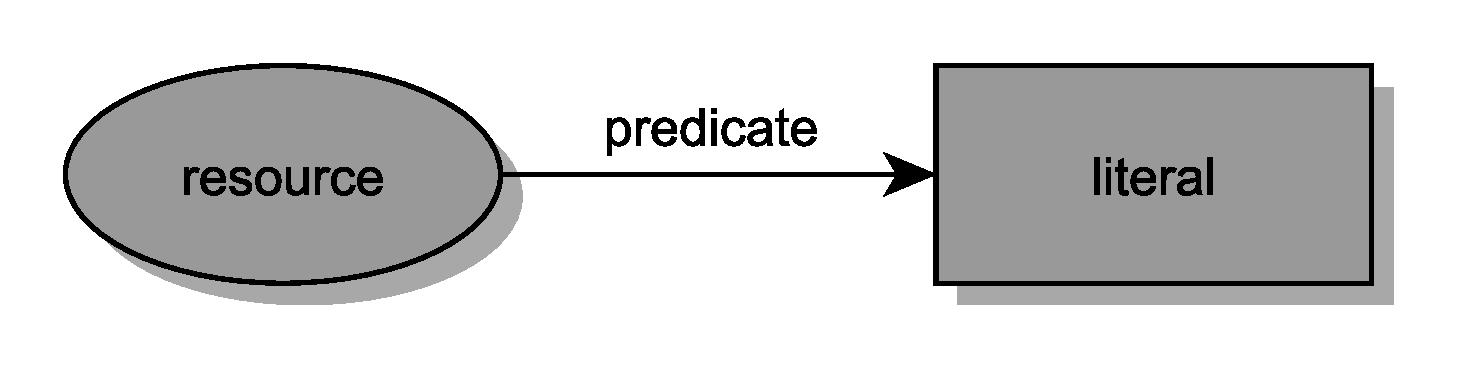
\includegraphics[
            width=0.6\textwidth,
            keepaspectratio=true,
            clip=true]
            {assets/images/rdf-triple}
        \caption{Einfacher RDF-Graph}
        \label{fig:graphisch_rdf_triple}
    \end{figure}

% paragraph graphische_darstellung (end)

\paragraph{RDF/XML} % (fold)
\label{par:rdf_xml}

RDF/XML ist eine verbreitete Form RDF-Dokumente zu beschreiben. Die Basis bildet hierbei die Verwendung von XML. In Listing \ref{lst:rdf_xml_beispiel} ist ein Beispieldokument in RDF/XML zusehen. Das in Zeile 2 zu sehende \texttt{rdf:RDF} ist das Wurzelelement für den RDF-Graphen. In diesem Wurzelelement werden mit \texttt{xmlns:\dots} einige Präfixe für Namensräume  definiert, um das Dokument übersichtlicher zu gestalten. Alle Präfixe werden danach mit den angegebenen Namensraum ersetzt. Das \texttt{Description} in Zeile 5 stellt die Beschreibung einer Ressource im RDF-Graphen dar. Die URI der Ressource wird mit dem Attribut \texttt{rdf:about} definiert. Innerhalb des Description-Elements befinden sich die Prädikate. In Zeile 6 steht also, dass die Ressource die Eigenschaft \texttt{exterms:enthaelt} hat und auf das Literal \texttt{Kekse} verweist. Wäre das Objekt nicht wie hier ein Literal sondern eine weitere Ressource, könnte man über das Attribut \texttt{rdf:ressource} für das \texttt{exterms:enthaelt} URI der Ressource angeben.

\begin{lstlisting}[
    language=XML,
    caption={RDF/XML Beispiel}\label{lst:rdf_xml_beispiel},
    captionpos=t]
<?xml version="1.0"?>
<rdf:RDF xmlns:rdf="http://www.w3.org/1999/02/22-rdf-syntax-ns#"
    xmlns:exterms="http://www.example.org/terms#">

    <rdf:Description rdf:about="http://www.example.org/dose">
       <exterms:enthaelt>Kekse</exterms:enthaelt>
    </rdf:Description>
</rdf:RDF>
\end{lstlisting}
% paragraph rdf_xml (end)

\paragraph{Turtle} % (fold)
\label{par:turtle}

Turtle\footnote{\url{http://www.w3.org/TeamSubmission/turtle/}} (Ausgeschrieben: \emph{Terse RDF Triple Language}) ist eine weiter Möglichkeit RDF-Graphen darzustellen und ging aus der Sprache N3\footnote{\url{http://www.w3.org/DesignIssues/Notation3.html}} (Kurzform für Notation 3) hervor. In Turtle wird das Triple aus Subjekt, Prädikat und Objekt hintereinander geschrieben und zwischen jeden mindestens ein Leerzeichen gelassen. Als Abschluss folgt nach jedem Tripel noch ein Punkt. Der Punkt verdeutlicht noch einmal die Ähnlichkeit mit gesprochenen Sätzen. Listing \ref{lst:turtle_beispiel} zeigt das Beispiel mit der Keksdose noch einmal in Turtle Notation. 

\begin{lstlisting}[
    caption={Turtle Beispiel}\label{lst:turtle_beispiel},
    captionpos=t]
<http://www.example.org/dose> <http://www.example.org/terms#enthaelt> "Kekse" .
\end{lstlisting} 


In Turtle ist darauf zu achten, dass alle URIs immer zwischen spitzen Klammern stehen müssen und Literale werden in Anführungszeichen geschrieben. Da nun einzelne Prädikate beziehungsweise allgemein URIs recht häufig innerhalb eines Graphen auftauchen können, kann es einfacher sein diese abzukürzen. Wie schon in RDF/XML können auch in Turtle Präfixe definiert werden, um Schreibarbeit zu sparen und den RDF-Graphen für Menschen lesbarer zu gestalten.

\begin{lstlisting}[
    caption={Turtle Präfixe}\label{lst:turtle_prefix},
    captionpos=t]
@prefix exterms: <http://www.example.org/terms#> .
<http://www.example.org/dose> exterms:enthaelt "Kekse" .   
\end{lstlisting}

In der ersten Zeile von Listing \ref{lst:turtle_prefix} wird durch Einleiten mit dem Schlüsselwort \texttt{@prefix} ein neuer Präfix \texttt{exterms:} für den Namensraum \texttt{http://www.example.org/terms\#} festgelegt. Dieser Präfix kann nun überall innerhalb des Dokumentes verwendet werden, wobei die spitzen Klammern dann weggelassen werden können.

\begin{lstlisting}[
    caption={Turtle abkürzende Schreibweise}\label{lst:turtle_shortcut},
    captionpos=t]
@prefix exterms: <http://www.example.org/terms#> .
<http://www.example.org/dose> exterms:farbe "blau";
    exterms:enthaelt "Kekse", "Geld" .   
\end{lstlisting}

Listing \ref{lst:turtle_shortcut} zeigt ein drittes Beispiel, wie redundante Angeben eingespart werden können. Wie man in der zweiten Zeile sehen kann, wird das Triple mit einem Semikolon abschlossen und nicht mit einen Punk. Durch das Semikolon ist es Möglich das Subjekt mehrfach wieder zu verwenden, wenn sich nur Prädikat und Objekt ändern. So können sich mehrere Eigenschaften einer Ressource platzsparend schreiben lassen ohne das Subjekt immer wieder anzugeben. Ändert sich dahingegen nur das Objekt, können mehrere durch Kommata getrennt hintereinander geschrieben werden. Die dritte Zeile beschreibt zum Beispiel, dass in der Dose nicht nur Kekse sonder auch Geld steckt. 

Leere Knoten können dann noch in Turtle durch angeben einer geöffneten eckigen Klammer gefolgt von einer sich Schließenden dargestellt \enquote{\texttt{[]}}. Zwischen diesen beiden Klammern kann zusätzlich eine Menge von Prädikaten und ihren Objekten stehen, die von Semikolons getrennt werden. Beispiele dazu sind im Anhang \ref{sec:anhang_proof_of_concept_konfigurationsdaten} zu sehen. Soll ein leerer Knoten innerhalb eines Graphen referenziert werden, kann er auch als \texttt{\_:LABEL}, wobei \texttt{LABEL} ein beliebiger Beizeichner ist, geschrieben werden.

% paragraph turtle (end)

% subsubsection darstellung_von_rdf (end)

% subsection semantic_web_und_das_resource_description_framework (end)

\subsection{Ontologien} % (fold)
\label{sub:ontologien}

Sollen Daten aus verschiedenen Quellen zusammengefügt werden, stellt sich häufig das Problem dass Teile dieser dieser Daten zwar den gleichen Sinn haben, aber aufgrund der Sichtweise des jeweiligen Systems eine andere Bezeichnung besitzen. Dies kann zum Beispiel zu Missverständnissen bei der Verarbeitung führen oder dass Teile eines anderen Systems nicht wiederverwendet werden können (vgl \cite{Uschold1996a}). Einen Ausweg aus diesem Dilemma kann die Verwendung von Ontologien zeigen. Ontolgien können allgemein als Wissensbasis \cite{Uschold1996a,Hitzler2008a} bezeichnet werden und liefern eine formale Spezifikation über eine bestimmte Interessensdömäne. Sie beschreibt nicht nur wie das verwendete Vokabular aussieht, sondern legt auch fest welche einheitliche Bedeutung jede Vokabel hat. 

Im Bereich des Semantic Webs sind heutzutage zwei Sprachen für die Erstellung von Ontologien verbreitet. Diese sind \emph{RDF Schema} (RDFS)\cite{Brickley} und die darauf aufbauende \emph{Web Ontology Language} (OWL)\cite{partelschneider2004}. Beide Sprachen basieren auf RDF, so können sie zusammen mit jedem System verwendet werden, das RDF versteht. Mit ihnen ist man im Stande abstrakte Klassen von Dingen und deren Eigenschaften zu definieren und diese in eine Vererbungshierarchie einzugliedern. Die Ausprägung eine Klasse wird als Individuum bezeichnet, in dieser Arbeit wird aber Begriff Objekt aus der objektorientierten Programmierung verwendet, um die Überleitung von der theoretischen Beschreibung zu Implementierung einheitlich zu halten. Im Gegensatz zu RDFS können in OWL diverse Einschränkungen definiert werden, wie zum Beispiel, dass eine Eigenschaft nur einmal pro Objekt einer Klasse vorhanden sein darf. Die Anhänge \ref{sec:anhang_socc_connector_config_ontologie} und \ref{sec:anhang_sioc_services_authentication_module} zeigen zwei Ontologien in der Sprache OWL, welche innerhalb dieser Arbeit entwickelt wurden und in Abschnitt \ref{sub:connector_config_ontologie} und \ref{sub:authentifizierung} beschreiben werden.

\subsubsection{Friend of a Friend (FOAF)} % (fold)
\label{ssub:friend_of_a_friend_}

Friend of a Friend\footnote{\url{http://www.foaf-project.org}} ist ein im Jahr 2000 gestartetes Projekt, das versucht Personen innerhalb des Webs, inklusive der Verbindungen zwischen ihnen und anderen, sowie dem was sie machen, in maschinenlesbarer Form abzubilden. FOAF stellt hierzu eine Ontologie \cite{Brickley2010} (RDF-Präfix \texttt{foaf:}) für solche sozialen Netzwerke zur Verfügung. Das Vokabular von FOAF gliedert sich dazu in einen \enquote{FOAF Core} und einen \enquote{Social Web} Bereich. Der Core-Bereich enthält die Klasse \texttt{foaf:Agent} für alle Dinge die eine Handlung ausführen können. Also sowohl natürliche Personen, Gruppen oder Organisationen, als auch Computerprogramme oder Maschinen. Für diese gibt es jeweils noch einzelne Unterklassen die von der Klasse \texttt{foaf:Agent} erben. Objekten dieser Klassen können eigene Eigenschaften wie einen Namen, ein Alter oder wen sie kennen gegeben werden. Der Sozial Web Bereich enthält alle Teile die für das Web interessant sind. Das wären zum Beispiel welche E-Mail-Adresse eine Person besitzt, welche Benutzerkonten ihm auf welcher Webseite gehören oder wie die URI seiner Homepage lautet. Das FOAF Projekt sieht sich aber selber nicht als Konkurrenz gegenüber den etablierten sozialen Online-Netzwerken, sondern eher ein Ansatz für einen besser Austausch zwischen den einzelnen Seiten \cite[siehe \enquote{Abstract}]{Brickley2010}.

Listing \ref{lst:foaf_beispiel} zeigt ein Beispiel FOAF-Dokument in RDF/XML. Es beschreibt die fiktive Person \enquote{Max Mustermann}, mit Vor- und Nachname sowie der Hashwert seiner E-Email-Adresse (\texttt{foaf:mbox\_sha1sum}). Diese Person kennt (\texttt{foaf:knows}) eine Person mit dem Namen \enquote{John Doe} der ebenso eine E-Mail-Adresse mit den angegeben Hashwert besitzt. Statt die Eigenschaften von John Doe hier noch einmal vollständig anzugeben, wird über die Eigenschaft \texttt{rdfs:seeAlso} auf ein weiteres FOAF-Dokument verwiesen, dass die fehlenden Daten enthält. 

\begin{lstlisting}[
    language=XML,
    caption={FOAF Beispiel}\label{lst:foaf_beispiel},
    captionpos=t]
<rdf:RDF xmlns:rdf="http://www.w3.org/1999/02/22-rdf-syntax-ns#"
         xmlns:rdfs="http://www.w3.org/2000/01/rdf-schema#"
         xmlns:foaf="http://xmlns.com/foaf/0.1/">
  <foaf:Person>
    <foaf:name>Max Mustermann</foaf:name>
    <foaf:firstName>Max</foaf:firstName>
    <foaf:surname>Mustermann</foaf:surname>
    <foaf:mbox_sha1sum>dce4fc922158f8b26fbf0a65ea32bfab58488bd2</foaf:mbox_sha1sum>
    <foaf:knows>
      <foaf:Person>
        <foaf:name>John Doe</foaf:name>
        <foaf:mbox_sha1sum>479ea35d3522662b70dc7afd721853485c95db57</foaf:mbox_sha1sum>
        <rdfs:seeAlso rdf:resource="http://www.example.org/people/jd/foaf.rdf"/>
      </foaf:Person>
    </foaf:knows>
  </foaf:Person>
</rdf:RDF>
\end{lstlisting}

% subsubsection friend_of_a_friend_ (end)

\subsubsection{Semantically-Interlinked Online Communities (SIOC)} % (fold)
\label{ssub:semantically_interlinked_online_communities}

Semantically-Interlinked Online Communities ist ein Projekt, welches von Uldis Boj\=ars und John Breslin begonnen wurde, um unterschiedliche, webbasierte Diskussionsplattformen(Blog, Forum, Mailinglisten,\dots) untereinander verbinden zu können (siehe \cite{deri2013,Breslin2005,Bojars2008a}). Der Kern von SIOC besteht aus einer Ontologie (RDF-Präfix \texttt{sioc:}), welche den Inhalt und die Struktur diese Plattformen in ein maschinenlesbares Format bringen kann und es erlaubt diese auf semantischer Ebene zu verbinden. Auch soll es so möglich sein Daten von einer Plattform zu einer Anderen zu transferieren und so einfacher Inhalte austauschen zu können. Als Basis für SIOC dient RDF, die Ontologie selber wurde in RDFS und OWL designt. Um nicht das Rad neu erfinden zu müssen greift SIOC auf schon bestehende und bewährte Ontologien zurück. Für die Abbildung von Beziehungen zwischen einzelnen Personen wird FOAF und für einige Inhaltliche- und Metadaten (Titel, Inhalt, Erstelldatum, \dots) Dublin Core Terms\footnote{\url{http://dublincore.org/documents/dcmi-terms}} eingesetzt.

\begin{figure}[ht]
    \centering
    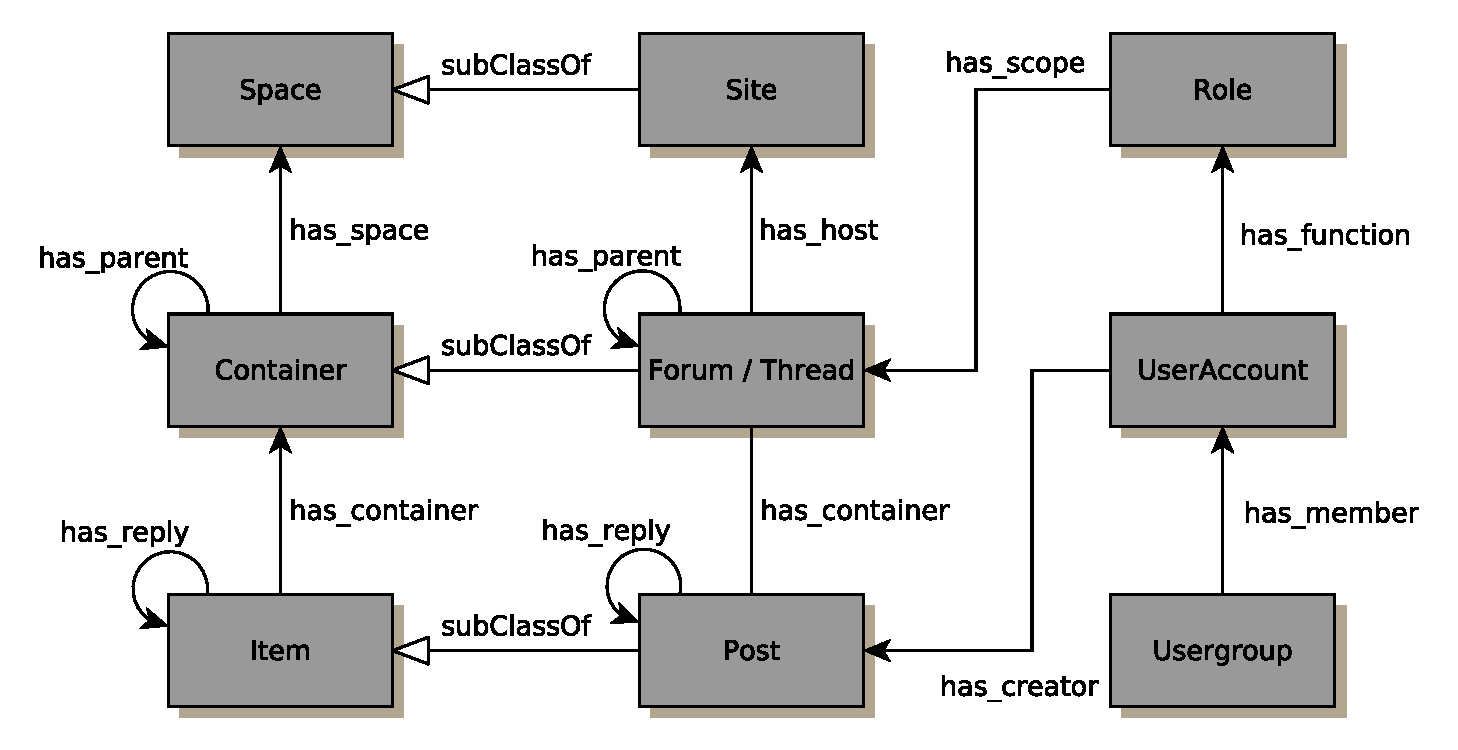
\includegraphics[
        width=\textwidth,
        keepaspectratio=true,
        clip=true]
        {assets/images/sioc_overview}
    \caption{Aufbau von SIOC (modifiziert) - Originalquelle: \cite{deri2013}}
    \label{fig:sioc_aufbau_diagramm}
\end{figure}

Die wichtigsten Klassen von SIOC sind in Abbildung \ref{fig:sioc_aufbau_diagramm} in der mittleren Spalte zu sehen. Die Klasse \texttt{sioc:Site} ist für die Beschreibung von Webseiten in denen Beiträge innerhalb von Containern verfasst werden. Ein solcher Container ist die Klasse \texttt{sioc:Forum} und steht für einen Ort an dem Beiträge geschrieben werden. Enthält ein Forum Diskussionen zu unterschiedlichen Themen, kann es noch einmal in \texttt{sioc:Thread} unterteilt werden, welche immer ein Forum als Elternteil haben müssen (\texttt{sioc:has\_parent}). Beide Klassen leiten sich von der Klasse \texttt{sioc:Container}, als einen allgemeinen Ort für Beiträge, ab. Die einzelnen Beiträge werden durch die Klasse \texttt{sioc:Post} beziehungsweise von der übergeordneten Klasse \texttt{sioc:Item} modelliert. Beiträge gehören in der Regel immer zu einen bestimmten Container oder mindesten zu einer Webseite. Es ist auch mögliche Beiträge als Kommentar zu anderen Beiträgen über die Eigenschaft \texttt{sioc:has\_reply} abzubilden (vgl. \cite[S.\,203ff]{Breslin2009}). Jeder Beitrag besitzt mindesten einen Autor der ein Benutzerkonto auf der betreffenden Seite besitzt. Für die Beschreibung eines solchen Benutzerkontos wird die Klasse \texttt{sioc:UserAccount} verwendet. Dieses Benutzerkonto kann zusätzlich zu einer Gruppe gehören. Über die Klasse \texttt{sioc:Role} kann einen Benutzerkonto eine bestimmte Rolle innerhalb einer Webseite, Forum und so weiter zugeteilt werden. Ein Beispiel dafür wäre die Rolle eines Moderator, der überwacht ob die Regel der Seite in den einzelnen Foren eingehalten werden.

% subsubsection semantically_interlinked_online_communities (end)

% subsection ontologien (end)

% section datenintegration (end)

\section{Datenaustausch} % (fold)
\label{sec:datenverteilung}

Sollen zwischen zwei unabhängigen Systemen Daten ausgetauscht werden, hat man im Allgemeinen mehrere Ansätze dieses Problem zu lösen. Beide Programme könnten Dateien mit den Daten an einen festen Ort speichern, die der jeweilig andere lesen kann. Auch ist das Benutzen eines gemeinsamen Datenbankmanagementsystems oder die Verwendung von RPCs denkbar. Ebenso ist der Datenaustausch mit Nachrichten über ein Netzwerk ein sehr flexibler und sicherer Weg. Jeder dieser Ansätze hat seine eigenen Vor- und Nachteile und sollte am Besten nach den Anforderungen für den Verwendungszweck gewählt werden. 

Dieser Abschnitt beschäftigt sich explizit nur mit dem Versenden und Empfangen von Nachrichten, da dies für das in der Einleitung beschriebene Wunschsystem die meisten Vorteile bringt. Dazu wird zuerst das \emph{Java Messageing Service} (JMS) vorgestellt und danach die Enterprise Integration Patterns (EIP) mit Apache Camel.

%\todo[inline]{Datenverteilung-Einleitung schreiben}

\subsection{Java Messaging Service} % (fold)
\label{sub:java_messaging_service}

Das JMS ist ein Sammlung von Schnittstellen für das Erstellen, Senden und Empfangen von Nachrichten zwischen Programmen. JMS erlaubt eine Entwicklung von verteilten Anwendung die nicht nur lose gekoppelt, sondern auch asynchron und zuverlässig arbeiten (vgl. \cite{jms}). 

\begin{figure}[ht]
    \centering
    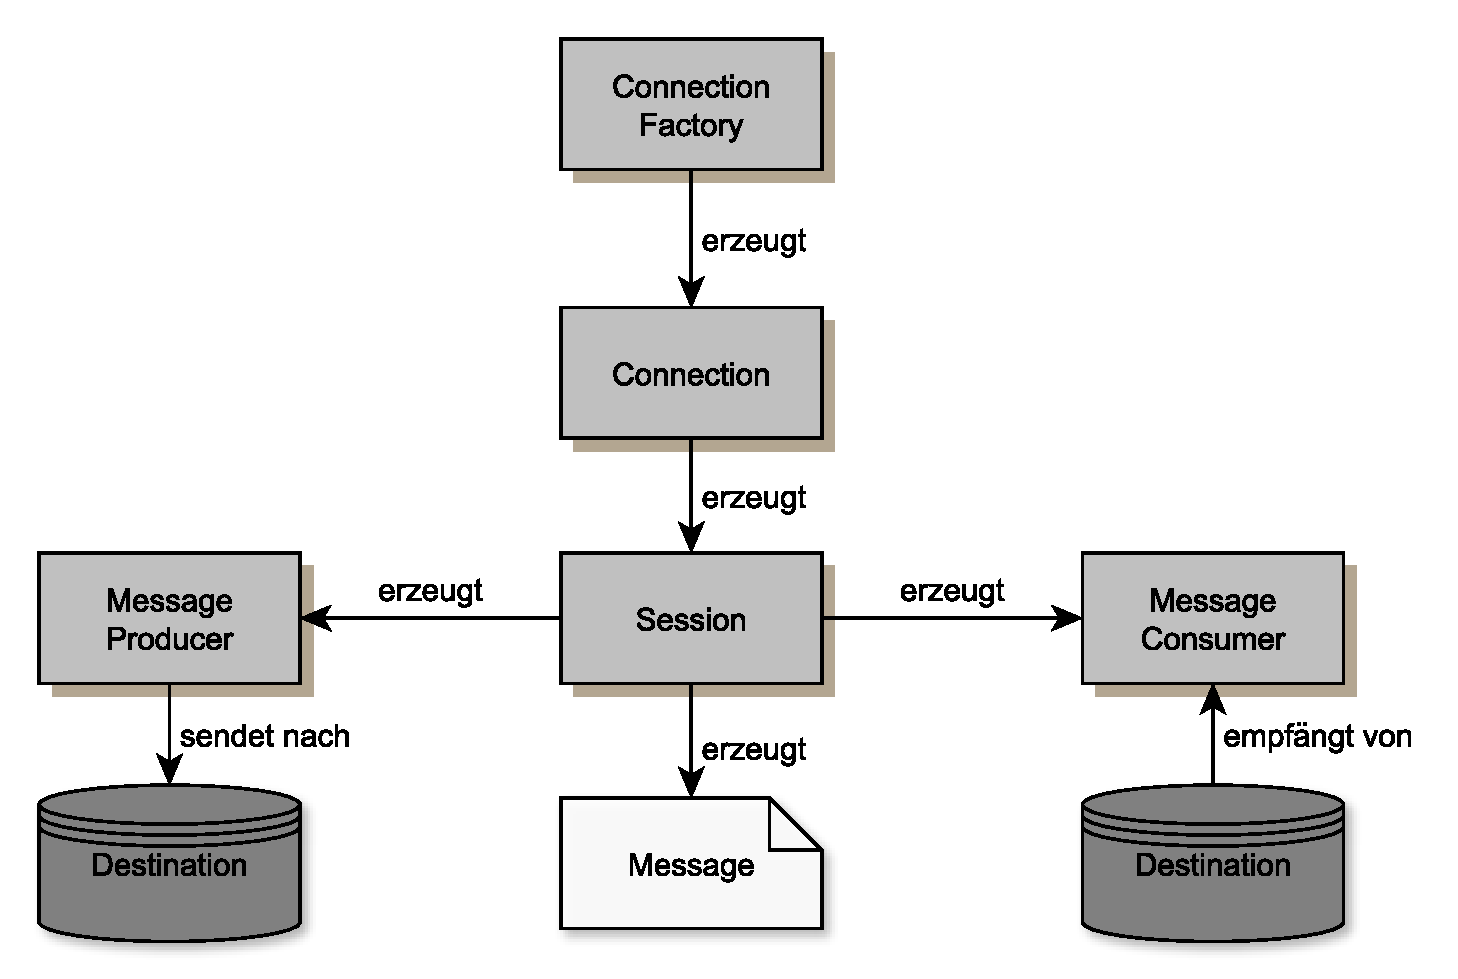
\includegraphics[
        width=0.8\textwidth,
        keepaspectratio=true,
        clip=true]
        {assets/images/jms_api_overview}
    \caption{JMS Programmiermodell - Original Bild: \url{http://docs.oracle.com/javaee/1.3/jms/tutorial/1_3_1-fcs/doc/images/Fig3.1.gif} (Zugriff: 2013-09-15)}
    \label{fig:jms_api_overview}
\end{figure}

Die Grundstruktur einer JMS Anwendung besteht aus einem \emph{JMS Provider}, der die Schnittstellen von JMS implementiert. Dieser JMS Provider wird auch als \emph{Message Oriented Middleware} (MOM) bezeichnet und kümmert sich auch darum, dass Nachrichten zuverlässig verschickt werden. Hinzu kommt ein JMS Client von dem Nachrichten verschickt und empfangen werden und die Nachrichten selber sowie sogenannte \emph{Administered Objects}. Diese Administered Objects bestehen aus vorkonfigurierten \emph{ConnectionFactory}s für das Erstellen von Verbindungen (\emph{Connection}) zwischen Client und Provider und \emph{Destination}s als Sende- und Empfangsendpunkte von Nachrichten. Die Administered Objects können im Client über das Java Naming and Directory Interface (JNDI)\footnote{JNDI API:\url{http://www.oracle.com/technetwork/java/index-jsp-137536.html}} API abgefragt werden. Alle Clients die nicht die JMS API sondern die implementierte API der MOM direkt verwenden, werden \emph{Native Client} genannt.

JMS unterstützt zwei Verbindungsarten zum Übertragen von Nachrichten: Queue- und Topic-basiert. Als Queue-basiert wird eine Punkt-zu-Punkt Verbindung bezeichnet. Hier werden Nachrichten nur zwischen zwei Clients übertragen und gegebenenfalls in einer Warteschlange zwischengespeichert. Hinter Topic-basiert verbirgt sich ein Publish-Subscribe-Mechanismus bei dem ein Client Nachrichten an eine Topic-Destination schickt und andere Clients sich auf dieses Topic anmelden können, um die dann die Nachrichten des ersten Clients zu empfangen. Ob Queue oder Topic-basiert, wird über die Art der Destination ausgewählt.

Sollen nun Nachrichten von einem Client verschickt beziehungsweise empfangen werden, muss mit einer ConnectionFactory eine neue Connection zu einer MOM aufgebaut werden. Mit dieser Connection wird danach eine \emph{Session} erstellt, das als Kontext zum Senden und Empfangen verwendet wird. Für das versenden von Nachrichten muss mit dem Sessionobjekt ein \emph{MessageProducer} erstellt werden. Für das Empfangen entsprechend einen \emph{MessageConsumer}. Abbildung \ref{fig:jms_api_overview} zeig noch einmal den Zusammenhang aller JMS Komponenten.

\begin{lstlisting}[
    caption={JMS Beispiel}\label{lst:jms_beispiel},
    captionpos=t]
Context ctx = new InitialContext();
ConnectionFactory connectionFactory = (ConnectionFactory) ctx.lookup("ConnectionFactory");

Connection connection = connectionFactory.createConnection();
connection.start();

Session session = connection.createSession();
Destination destination = session.createTopic("topic-test");

MessageProducer msgProducer = session.createProducer(destination);
Message msg = session.createTextMessage("Hallo World!");
msgProducer.send(msg);
\end{lstlisting}

Listing \ref{lst:jms_beispiel} zeig ein kleines Beispiel zum Senden eine Textnachricht mit JMS. Die erste und zweite Zeile zeigt wie ein JNDI Kontext erstellt und nach einer vordefinierten ConnectionFactory mit den Name \enquote{ConnectionFactory} gesucht wird. Mit dieser ConnectionFactory wird dann eine neue Connection erstellt und gestartet. Danach folgt in Zeile 7 und 8 das Erstellen einer neuen Session und die Definition eins Topics mit dem Namen \enquote{topic-test} als Destination. In der zehnten Zeile wird dann der MessageProducer zum Senden von Nachrichten und in der Folgezeile die zu sendende Textnachricht erzeugt. Diese wird dann in der letzten Zeile vom MessageProducer an das Topic verschickt.

% subsection java_messaging_service (end)

\subsection{Enterprise Integration Patterns (EIP)} % (fold)
\label{sub:enterprise_integration_pattern}

Bezeichnungen wie \enquote{Iterator}, \enquote{Factory Method}, \enquote{Observer} oder \enquote{Proxy} hat bestimmt schon jeder Programmieren mindestens einmal gehört. Hierbei handelt es sich im sogenannte Entwurfsmuster für Softwareprogramme. Sie sind Schablonen für Lösungen von Problemen, die in der Entwicklung von Software immer wieder auftreten und sich als hilfreich erwiesen haben. Auch in der Integration von verschiedenen Geschäftsanwendungen in ein System treten solche Muster immer wieder auf. Gregor Hohpe und Bobby Woolf beschreiben in ihren Buch \enquote{Enterprise Integration Patterns: Designing, Building, and Deploying Messaging Solutions}\cite{Hohpe:2003:EIP:940308} eine Vielzahl solcher EIP für die Integration mittels MOM. Alle hier aufzuzählen würde jedoch den Rahmen dieser Arbeit sprengen. Aus diesem Grund werden in Tabelle \ref{tbl:eip_beispiel_muster} fünf Muster inklusive der verwendeten Symbole vorgestellt, die später noch vorkommen werden. Die restlichen Muster sind auf der Webseite der EIP\footnote{\url{http://www.enterpriseintegrationpatterns.com/toc.html}} zu finden.

\begin{table}[ht]
    \centering
    \caption{Einige Beispiel von EIP}
    \begin{tabular}{c|c|p{9cm}}
        \textbf{Icon} & 
        \textbf{Name} & 
        \textbf{Beschreibung} \\ 
        \hline

        \raisebox{-0.7\totalheight}{
\includegraphics[
            width=1cm,
            keepaspectratio=true]
        {assets/images/eip/message_alt}} & 
        \emph{Message} & 
        Über Nachrichten werden Daten zwischen zwei oder mehr Systemen ausgetauscht. \\

        \raisebox{-0.7\totalheight}{
\includegraphics[
                width=3cm,
                keepaspectratio=true]
            {assets/images/eip/channel}}& 
        \emph{Channel} &
        Ein Channel beschreibt einen Nachrichtenkanal über den Nachrichten von einem System in ein anderes verschickt werden können.\\

        \raisebox{-0.7\totalheight}{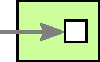
\includegraphics[
                width=3cm,
                keepaspectratio=true]
            {assets/images/eip/endpoint}}& 
        \emph{Endpoint} & 
        Endpoints sind Schnittstellen in einem System, von dem Nachrichten in einen Kanal gesendet oder von dort Empfangen werden. \\
        &&\\


        \raisebox{-0.7\totalheight}{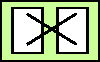
\includegraphics[
                width=3cm,
                keepaspectratio=true]
            {assets/images/eip/message_translator}} & 
        \emph{Message Translator} & 
        Nicht immer liegt eine Nachricht im richtigen Format für ein System vor. Durch Message Translators können diese in das gewünschte Format konvertiert werden.\\

        \raisebox{-0.7\totalheight}{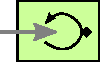
\includegraphics[
                width=3cm,
                keepaspectratio=true]
            {assets/images/eip/polling_consumer}} &
        \emph{Polling Consumer} &
        Manchmal ist möchte ein Programm Nachrichten nicht verarbeiten wenn sie ankommen, sondern dann wenn es bereit dazu ist. Ein PollingConsumer fragt also erst zu bestimmten Zeitpunkten ab, ob Nachrichten für in vorliegen. 
    \end{tabular}
    \label{tbl:eip_beispiel_muster}
\end{table}

\subsubsection{Apache Camel} % (fold)
\label{ssub:apache_camel}

\emph{Apache Camel}\cite{ApacheCamel} (kurz: Camel) ist ein Projekt der Apache Software Foundation (kurz: Apache) für das Routen und Verteilen von Nachrichten zur Integration von System auf Basis von definierten Regeln. Camel stellt dazu eine Java-basierte API für den Einsatz der EIP bereit. Die Regeln für die Routen, die Nachrichten nehmen können, können direkt in Java, aber auch durch das Spring Framework\footnote{\url{http://www.springsource.org/}} in XML definiert werden. 

\begin{lstlisting}[
    caption={Apache Camel Beispiel}\label{lst:camel_beispiel},
    captionpos=t]
RouteDefinition rd = new RouteDefinition()
    .from('timer://helloTimer?period=3000')
    .to('log:helloLog');

CamelContext camelContext = new DefaultCamelContext();
camelContext.addRouteDefinition( rd );
camelContext.start();
\end{lstlisting}

Listing \ref{lst:camel_beispiel} zeig ein Beispiel, wie eine Nachrichtenroute in Java für Camel definiert werden kann. In der ersten Zeile wird über die Klasse \texttt{RouteDefinition} eine neue Route erstellt. Über die Methode \texttt{from} wird der Endpunkt, vom dem die Route ausgeht, festgelegt. Welcher Endpunkt das genau seien soll kann auf zwei Arten definiert werden. Man übergibt der Methode direkt ein Objekt einer Klasse die das Interface \texttt{Endpoint} implementiert oder man macht es, wie hier im Beispiel, über eine URI. Diese URI baut sich auf folgende Weise zusammen: Der Teil bis zum Doppelpunkt, das sogenannte \enquote{Schema}, legt die Komponente (engl. \texttt{Component}) fest, von der ein Endpunkt erzeugen werden soll. In diesem Falls ist es eine Timer-Komponente, deren Endpunkt im periodischen Abstand Event-Nachrichten verschickt. Der Rest der URI wird zur Konfiguration an den Endpunkt übergeben. \enquote{helloTimer} steht hier für einen Namen für den Timer und der Parameter \enquote{period} gibt den zeitlichen Abstand zwischen zwei Event-Nachrichten an. Das Ziel der Route wird mit der Methode \texttt{to} in Zeile 3 festgelegt. Für das Ziel wird hier eine Log-Komponente mit dem Namen \enquote{helloLog} festgelegt, die alle reinkommenden Nachrichten protokolliert. In der fünften Zeile wird ein \texttt{CamelContext} Objekt, das für die Verwaltung und Ausführung der Routen verantwortliche ist, erstellt. Die Route wird dann dem CamelContext hinzugefügt und die Ausführung in der letzten Zeile gestartet. Nun wird der Timer alle 3000 Millisekunden eine neue Event-Nachricht erzeugen und an den CamelContext schicken. Dieser leitet die Nachricht dann an das durch die Route definierte Ziel und wird dort von der Log-Komponente ausgeben.

Für Camel existieren schon eine Menge vorgefertigter Komponenten\footnote{\url{http://camel.apache.org/components.html}} die ein großes Spektrum an Anwendungsmöglichkeiten abdeckt. Es gibt Komponenten für die Anbindung an HTTP-Webserver, JMS-Provider, E-Mail-Server, RSS/Atom-Feeds und viele mehr. 

% subsubsection apache_camel (end)

% subsection enterprise_integration_patternl (end)

% section datenverteilung (end)

\section{Lernplattformen und soziale Online-Netzwerke} % (fold)
\label{sec:lernplattformen_und_soziale_online_netzwerke}

An dieser Stelle sollen kurz einige Lernplattformen und soziale Online-Netzwerke vorgestellt, die im späteren Verlauf dieser Arbeit für die Implementierung verwendet wurden. Im Einzelnen waren dies \emph{Moodle}, \emph{Canvas}, \emph{Facebook}, \emph{Google+} und \emph{Youtube}, da sie einen guten Schnitt von den Plattformen bilden, die heutzutage sowohl im Bereich E-Learning als auch von der breiten Masse verwendet werden.

\subsection{Moodle} % (fold)
\label{sub:moodle}
%% korrigiert am 2013-10-01

Moodle\footnote{\url{https://moodle.org/}} ist ein weit verbreitetes Open Source Online LMS. Die Hauptaufgabe liegt im Verwalten von Online-Kursen im Bereich E-Learning. Hierzu bietet Moodle von Haus aus eine große Menge an Funktionen für die Verwaltung des Kurses und die Kommunikation zwischen Lehrenden und Lernenden. Es bietet die Möglichkeit Aufgaben an die Teilnehmer zu verteilen, Fragebögen zu erstellen, zusätzlichen Kursmaterialien bereitzustellen und den Lernerfolg durch Benotung und Feedback zu kontrollieren. Funktionen für die Unterstützung des kollaborativen Lernens sind ebenfalls vorhanden. Teilnehmer können Lerngruppen bilden, sich über persönliche Nachrichten austauschen, gemeinsam an Wikis arbeiten oder in Foren diskutieren. 
% \begin{figure}[ht]
%     \centering
%     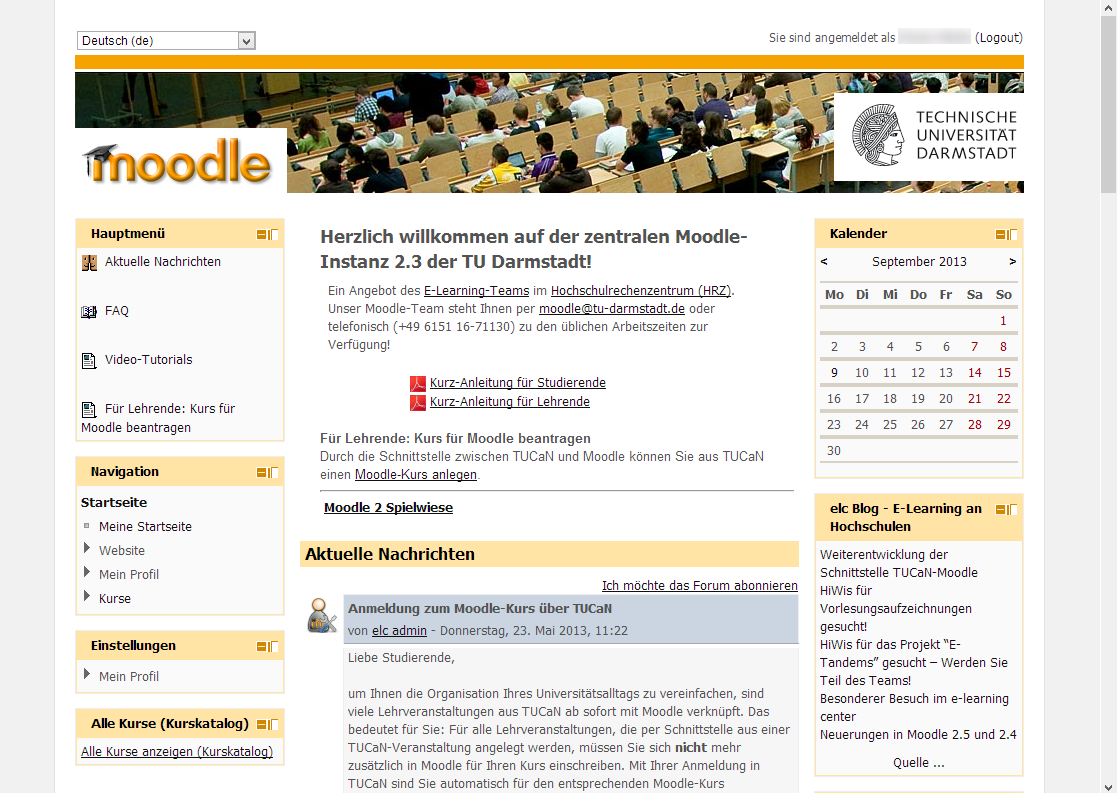
\includegraphics[
%         width=0.7\textwidth,
%         keepaspectratio=true,
%     ]{assets/images/tud_moodle_screenshot}
%     \caption{Moodleinstanz der TU Darmstadt}
%     \label{fig:moodle_tud}
% \end{figure}

Moodle wurde in der Programmiersprache PHP geschrieben und unterstützt die  Datenbanken MySQL, PostgrSQL, MSSQL und Oracle. Die Installation von weiteren Funktionalitäten ist durch von Dritten geschriebenen Erweiterungen möglich. Seit Version 2.0 können für Moodle auch Webservices installiert werden. So können auch externe Anwendungen auf interne Funktionen und Daten zugreifen.

% subsection moodle (end)

\subsection{Canvas} % (fold)
\label{sub:canvas}

Das von der Firma Instructure\footnote{\url{https://www.instructure.com}} entwickelte \emph{Canvas} ist ein recht neues, unter Open Source Lizenz gestelltes LMS. Vom Funktionsumfang ist es Moodle nicht unähnlich. Es existiert eine Verwaltung einzelner Kurse. Innerhalb dieser Kurse können in einem Forum Diskussionen geführt und Lernmieteralien hoch- und heruntergeladenen werden. Verteilung von Aufgaben, deren Benotung und ein Benachrichtigungssystem existiert ebenfalls. Canvas erlaubt auch das Einbinden von externen Diensten zum kollaborativen Lernen und Arbeiten wie Google Docs\footnote{\url{https://drive.google.com}} oder der Webkonferenz Anwendung BigBlueButton\footnote{\url{http://www.bigbluebutton.org}}.

% \begin{figure}[ht]
%     \centering
%     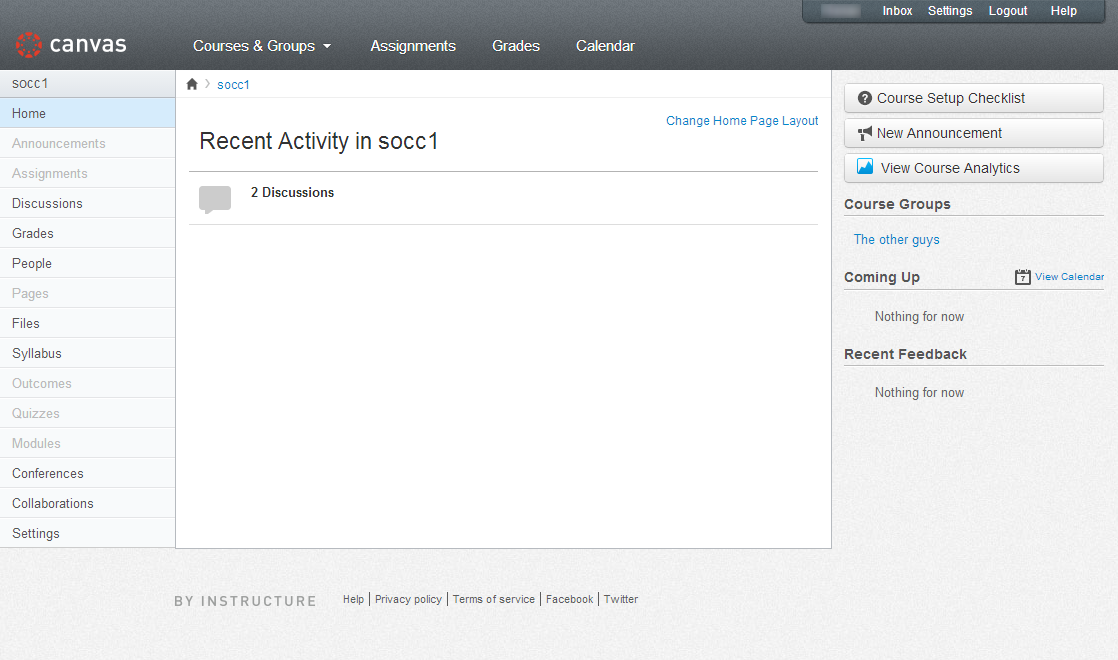
\includegraphics[
%         width=0.7\textwidth,
%         keepaspectratio=true,
%     ]{assets/images/canvas_lms}
%     \caption{Instructure Canvas}
%     \label{fig:canvas_lms}
% \end{figure}

Canvas wird mittels des Webframeworks \emph{Ruby on Rails}\footnote{\url{http://rubyonrails.org}} entwickelt. Das Aussehen ist etwas moderner, als das von Moodle und es wird sehr stark auf die neuesten Webtechnologien wie HTML5 CSS3 und JQuery gesetzt. Eine Erweiterung der Funktionalität von Canvas ist durch das einbinden von Programmen möglich, die den \emph{Learning Tools Interoperability™} (LTI) Standard erfüllen. Einige solcher Programme finden sich auf der Webseite \url{https://www.edu-apps.org}. Unter anderem Programme zum Suchen und Einbinden von Youtube Videos, Wikipedia Artikeln, GitHub Gists\footnote{\url{https://gist.github.com}} und vielen weiteren.

% subsection canvas (end)

\subsection{Youtube} % (fold)
\label{sub:youtube}

Youtube\footnote{\url{https://www.youtube.com}} gehört wohl heute zu den beliebtesten Anlaufpunkten im Internet, wenn es um das Thema Videos geht. Monatlich nutzen über 1 Milliarde Nutzer die Seite und pro Minute werden 100 Stunden neuer Videos hochgeladen (siehe \cite{youtube2013statistics}). Doch nicht das komplette Videomaterial besteht aus Katzen, Musik oder Unfallvideos. Ein Teil der Benutzer, die eigene Videos hochladen, wollen anderen Dinge beibringen, weil es in ihr Interessengebiet passt oder früher selber Probleme damit hatten. Einer erklärt die Logarithmengesetze, ein anderer wie man Feuer ohne Feuerzeug macht und eine ganz andere gibt Schönheitstipps. Youtube ist also auch im E-Learning Bereich gut einsetzbar. Lehrende können eigene Videos hochladen, von anderen interessante Videos in Playlisten zusammenfassen und die Lernenden können über Kommentare Fragen zum Inhalt stellen. 

% subsection youtube (end)

\subsection{Facebook} % (fold)
\label{sub:facebook}
%% korrigiert am 2013-10-01

Das soziale Online-Netzwerk Facebook\footnote{\url{https://www.facebook.com/}} kann mit rund 699 Millionen aktiven Benutzern täglich zu den aktuell beliebtesten Vertretern seiner Art bezeichnet werden (siehe \cite{Facebook2013}). Facebook erlaubt es, wie alle sozialen Online-Netzwerke, bekannte Personen in Freundeslisten zusammen zufassen und mit ihnen private Nachrichten auszutauschen. Beiträge wie Texte, Fotos oder Videos können auf einer Art Pinnwand, der \enquote{Wall}, öffentlich oder nur mit Freunden geteilt werden. Benutzer mit gemeinsamen Interessen können dazu eigene Gruppen bilden und dort auf einer eigen Wall Beiträge veröffentlichen oder die anderer kommentieren. Wie in der Einleitung schon erklärt zeigt Qiyun Wang et. al. \cite{Wang2012} das sich Facebook, wenn auch mit Einschränkungen, wunderbar zur Verwaltung und Nutzung durch Lernkurse und Lerngruppen eignet. Die gleiche Erfahrung teilte Anthony Fontana \cite{Fontana2009,FacebookinEducarion2010}, der Facebook als Alternative zum bestehenden System der Bowling Green State University in Ohio, USA verwendete.

% subsection facebook (end)

\subsection{Google+} % (fold)
\label{sub:google_plus}
%% korrigiert am 2013-10-01

Google+\footnote{https://plus.google.com} ist ein 2011 von Google gestartetes soziales Online-Netzwerk. Seit Anfang 2013 ist Google+, von der Anzahl der aktiven Benutzer her gesehen, auf Platz 2 hinter Marktführer Facebook (siehe \cite{Thomas2013}). Vom Funktionsumfang sind sich beide sehr ähnlich. Auf Google+ können andere Benutzer in sogenannten \enquote{Circles} sortiert werden, welche den auf Facebook genutzten Freundeslisten entspricht. Jeder Benutzer hat einen eigenen \enquote{Stream} in dem er Beiträge öffentlich oder nur für ein oder mehrere Circles verfassen kann. Das Gründen von Gruppen für bestimmte Interessensbereiche ist auch in Google+ möglich und werden dort als \enquote{Communities} bezeichnet. Eines der interessantesten Funktionen von Google+ dürfte die Einführung von \enquote{Google Hangout} sein. Hier können Benutzer neben Chats auch Videokonferenzen mit bis zu zehn anderen abhalten, ohne einen externen Service wie Skype\footnote{\url{http://www.skype.com/}} zu nutzen. Diese Funktion wäre gut für den Einsatz in E-Learning nutzbar. Ein Tutor könnte so in kleiner Runde Fragestunden oder Gruppen Treffen abhalten.

% subsection google_ (end)

% section lernplattformen_und_soziale_online_netzwerke (end)

\section{Verwandte Arbeiten und Projekte} % (fold)
\label{sec:verwandte_arbeiten_und_projekte}

Leider gibt es so gut wie kein Projekt, dass sich direkt mit den Austausch von Diskussionsbeiträgen zwischen unterschiedlichen Plattformen befasst. Ein dieser der doch existierenden Projekte wurde weiter oben mit SIOC in Verbindung mit FOAF schon vorgestellt. Nichtsdestotrotz existieren Arbeiten und Projekte die sich damit befassen, wie jeder seine Daten, die er irgendwann und irgendwo in einen sozialen Online-Netzwerk hinterlassen hat, wieder zurück unter seine Kontrolle bringt. Von diesem Punkt ist es nicht mehr weit, diese Daten wieder in eine andere Plattform zu übertragen, falls dies gewünscht ist.  
%\todo[inline]{Verwandte Arbeiten Einleitung schreiben}

\subsection{What happens when Facebook is gone?} % (fold)
\label{sub:what_happens_when_facebook_is_gone}

Frank McCown und Michael L. Nelson beschreiben in ihrem Bericht \enquote{What happens when Facebook is gone?}\cite{McCown2009}, wie Möglichkeiten aussehen können, die unsere Daten von sozialen Online-Netzwerken (hier im speziellen Fall von Facebook) für uns und die Nachwelt archivieren können. Zum Beispiel, wenn eine Person einen großen Teil seines persönlichen Lebens auf Facebook verbringt und plötzlich stirbt. Wie sollen seine Angehörigen an nicht öffentliche Texte, Bilder, Videos heran kommen, wenn sie in der Regel keinen Zugriff auf das Benutzerkonto haben, da der Verstorbene so etwas nicht vorhersehen konnte. Oder wenn ein Benutzer mit seinen Daten in ein anderes soziales Online-Netzwerk umziehen will, sei dies bei Facebook (zum damaligen Zeitpunkt) nur schwer möglich.

\begin{quote}
    \enquote{It is also likely he was not prepared to die at such a young age, and much of his personal life, which lies in the digital \grqq cloud\grqq, may never be accessible to his loved ones}
    \cite[S.\,251]{McCown2009}
\end{quote}

Zum Anlegen eines solchen Archivs wurden mehrere Ansätze vorgestellt. Die einfachste Ansatz wäre die E-Mail-Benachrichtigung zu aktivieren und alle neuen Beiträge in einem E-Mail-Postfach zu sichern. So können aber nur alle neuen Beiträge erfasst werden. Alte bleiben weiterhin in Facebook. Eine sehr aufwändige Möglichkeit wäre es Bildschirmfotos von den Beiträgen zu machen und diese durch ein Texterkennungsprogramm laufen zu lassen. Die dadurch erzeugten Dateien können dann in einer Datenbank gespeichert werden. Heutige Internetbrowser bieten es zusätzlich zum Anzeigen von Webseite auch das Herunterladen selbiger an. Dabei wird die HTML-Datei inklusive aller darin enthaltenen weiteren Dateien wie Bilder, Videos und CSS-Dateien gespeichert. Die so archivierte Seite hat dann im beschränkten Umfang genau das gleiche Aussehen und Verhalten wie die original Seite. Ebenfalls wäre eine Nutzung der von Facebook bereitgestellten API für Anwendungen eine Überlegung wert. 2009 war diese API noch sehr eingeschränkt. Gerade der Zugriff auf Beiträge und private Nachrichten war nicht möglich (siehe \cite[S.\,253, Table 1]{McCown2009}). Für die Implementierung eines Beispiel Programms wurde ein fünfter Ansatz gewählt. Über einen sogenannten Webcrawler oder eine Erweiterung für den Browser werden relevante Seiten automatisch heruntergeladen und in einen Archiv abgelegt. Dynamische Inhalte sollen kein Problem darstellen, da Seite erst heruntergeladen wird, wenn alle Aufrufe dynamischer Funktionen abgeschlossen ist. Die archivierten Dateien können dann mittels Datamining Techniken verarbeitet und als Atom/RSS Feed\footnote{\url{http://www.rssboard.org/rss-specification}} bereitgestellt werden. 

% subsection what_happens_when_facebook_is_gone_ (end)

\subsection{Reclaim Social} % (fold)
\label{sub:reclaim_social}

Ein Problem bei der heutigen Landschaft an sozialen Online-Netzwerken ist die Tatsache, dass man nicht nur ein einziges für alles Benutzt, sondern mehrere Gleichzeitig. Einige davon fast täglich andere werden immer weniger genutzt und irgendwann vergessen. Zugleich ist alles was man dort geschrieben oder hochgeladen hat auf den Server der Betreiber \enquote{gefangen}. Genau aus diesem Grund haben Sascha Lobo und Felix Schwenzel auf der Netzkonferenz re:publica\footnote{\url{http://re-publica.de/}} 2013 ihr Projekt \enquote{Reclaim Social} \cite{Schwenzel2013} vorgestellt.

Ziel dieses Projektes ist es von einen selber erzeugten sozialen Daten aus allen möglichen Quellen auf seinen eigenen Blog zu spiegeln und so einen zentrale Anlaufstelle für seine eigenen Inhalte schaffen. Reclaim Social baut dazu auf der weit verbreiteten Blogsoftware \enquote{WordPress\footnote{\url{http://wordpress.org/}}} und der dafür vorhandenen Erweiterung \enquote{FeedWordPress}\footnote{\url{http://feedwordpress.radgeek.com/}} auf. Diese Kombination ermöglichst alle Internetseiten, welche einen RSS/Atom-Feed anbieten, in die Datenbank von WordPress zu überführen. Das Problem hierbei besteht darin, dass einige sehr beliebte Internetseiten solche RSS/Atom-Feeds nicht anbieten (Facebook, Google+) oder eingestellt haben (\url{https://twitter.com}). Für einige solcher Seiten wurden \enquote{proxy-scripte}\cite[\enquote{Tech Specs Details}]{Schwenzel2013} implementiert, welche für diese einen RSS Feed emulieren. Zugleich können in den Feeds enthaltende Medien, wie Bilder und Videos (bisher nur als Referenz), heruntergeladen und in WordPress gespeichert werden. So ist es möglich alle gespiegelten Daten einfach zu durchsuchen oder nach bestimmten Kriterien zu filtern. Zusätzlich können alle Freunde, welche auch Reclaim Social einsetzen, in einen Kontaktliste eingetragen und so auch deren Inhalte eingebunden werden.

Aktuell befindet sich dieses Projekt noch im Alphastadium und die Installation ist relativ kompliziert. Es ist aber geplant eine eigene Erweiterung für WordPress zu schreiben \enquote{The goal is to build just one Reclaim Social-plugin for any wordpress user}\cite[\enquote{How Does It Work}]{Schwenzel2013}

% subsection reclaim_social (end)

% section verwandte_arbeiten_und_projekte (end)

% chapter grundlagen (end)
		%!TEX root = ../thesis.tex

\chapter{Analyse} % (fold)
\label{cha:analyse}

%\todo[inline]{Inhalt: wass gibt es, was muss neu gemacht werden}
\todo[inline]{Aufteilen in Szenarien: Datenaustausch, Übertragung...}

Bevor nun ein System entwickelt werden kann, das die Synchronisation von Diskussionen auf Lernplattformen und sozialen Online-Netzwerken ermöglicht, muss erst analysiert werden, welche Aufgaben das System erfüllen muss und welche Techniken dafür geeignet sind. Alle diese Schritte sollen im folgenden Abschnitt an einen kleinen Beispiel gezeigt werden.

\section{Ein Beispiel} % (fold)
\label{sec:analyse_beispiel}

% section neuen_beitrag_verfassen (end)
Am Anfang muss jemand auf einer Webseite einen Beitrag schreiben der synchronisiert werden kann. Zum Beispiel geht ein Student in das Forum seiner Veranstaltung auf der Webseite A und in den Thread zur aktuellen Übung, weil er zu ihr eine Frage hat. Er schreibt also einen neuen Beitrag in das Eingabefeld und schickt es ab. Dieser wird dann an die Webseite A geschickt, im dortigen Format (Format A) in eine Datenbank oder Ähnliches geschrieben und als neuer Beitrag im Thread angezeigt (siehe Abbildung \ref{fig:beutzer_erstellt_beitrag_a}). Da eine andere Webseite B das Format von Webseite A in der Regel nicht versteht, muss in einen nächsten Schritt der Beitrag aus der Datenbank gelesen und auf irgendeine Art konvertiert werden. 

\begin{figure}[ht]
     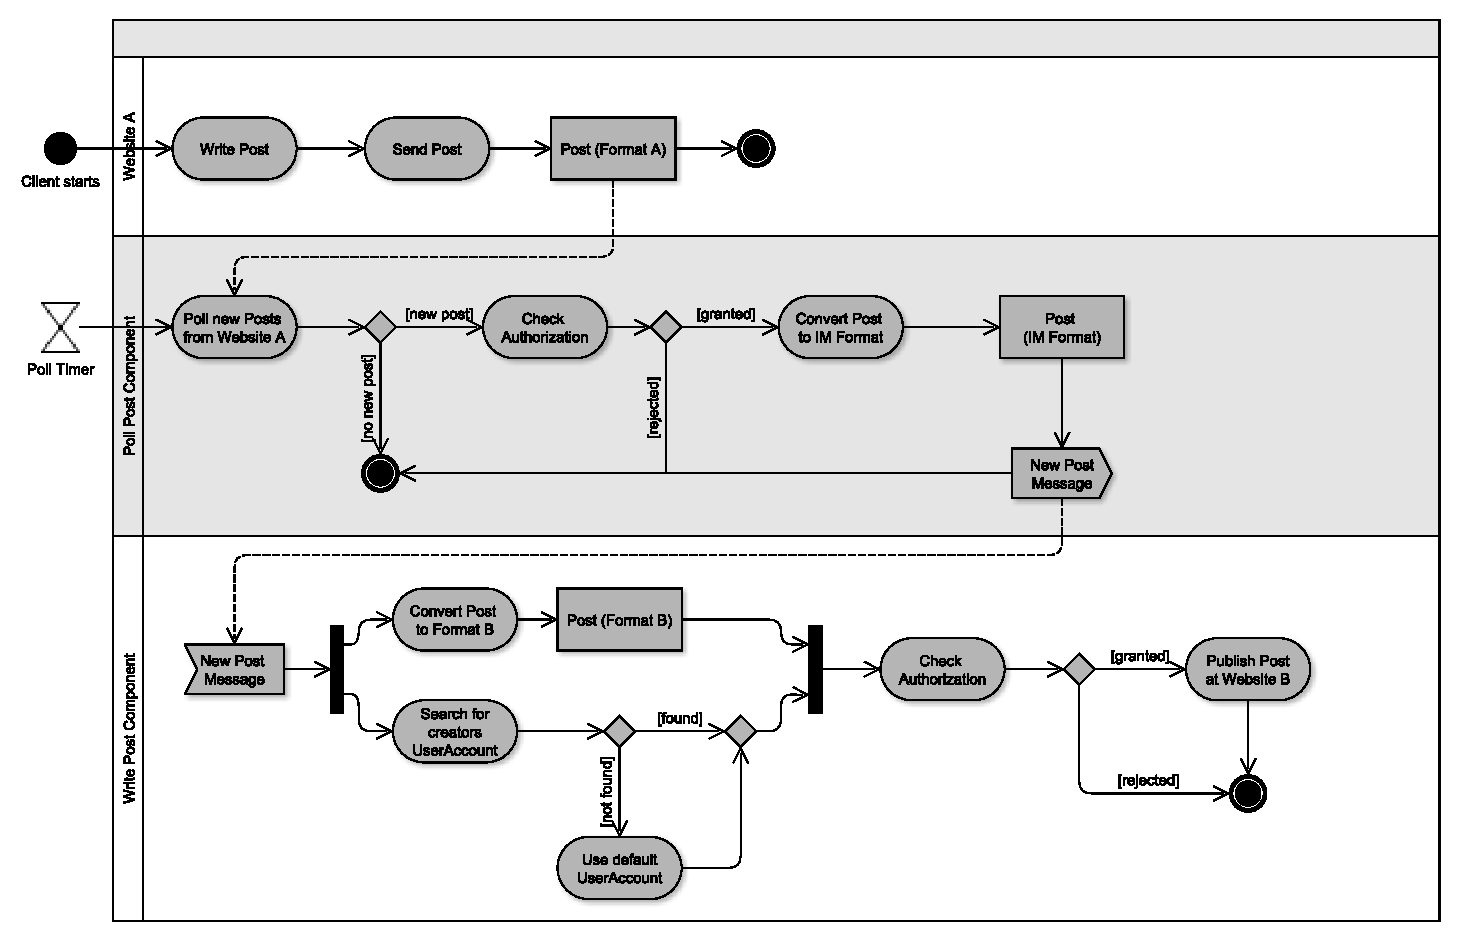
\includegraphics[
        width=\textwidth,
        keepaspectratio=true,
        clip=true,
        trim= 0 338 0 27
    ]{assets/images/activitydiagram_post_as_user_check_authorization.pdf}
    \caption{Benutzer erstellt einen Beitrag im sozialen Netzwerk A.}
    \label{fig:beutzer_erstellt_beitrag_a}
\end{figure}

\subsection{Beiträge lesen und konvertieren} % (fold)
\label{sub:beiträge_lesen_und_konvertieren}

Abbildung \ref{fig:lesen_von_beitrag_und_convertieren} zeigt den Ablauf, wie Beiträge von der Webseite A gelesen, konvertiert und weiterverarbeitet werden. Dazu müssen zuerst die Daten über eine öffentliche API vom Server des Webseite A heruntergeladen werden. Da im Allgemeinen nicht automatisch bekannt ist, wann ein neuer Beitrag vorhanden ist, müssen die Server in zeitlichen Abständen abgefragt (\emph{Polling} genannt) und die zurückgelieferten Daten nach neuen Beiträgen durchsucht werden. Sind ein oder mehrere neue Beiträge gefunden worden, können diese nicht direkt an die Webseite B geschickt werden, da sich diese in der Regel im verwendeten Datenformat unterscheiden. Diese müssen zuvor konvertiert werden.

Die einfachste Möglichkeit wäre die Daten von Webseite A, die in Format A vorliegen, in das Format B von Webseite B zu konvertieren. Bei zwei Formaten ist dies noch sehr einfach. Es müsste lediglich ein Konverter von Format A nach Format B und einer in die umgekehrte Richtung implementiert werden. Für den Fall, dass ein weiteres Webseite C unterstützt werden soll, würde ich die Anzahl an notwendigen Konvertern , wie Tabelle \ref{tbl:anzahl_konvertern_bei_drei_netzwerken} zeigt, auf Sechs erhöhen.

\begin{table}[ht]
    \centering
    \caption{Anzahl Konverter bei drei Webseiten}
    
    \begin{tabular}{c|c|c|c|c}
        % Zeile 1
        \multicolumn{2}{c|}{\multirow{2}{*}{}} & 
        \multicolumn{3}{|c}{\textbf{Nach}}   \\ 
        \cline{3-5} 

        % Zeile 2
        \multicolumn{2}{c|}{} & 
        \textbf{Webseite A} & 
        \textbf{Webseite B} & 
        \textbf{Webseite C} \\ 
        \hline

        % Zeile 3
        \multirow{3}{*}{Von} & 
        \textbf{Webseite A} & 
        -&            
        $ \times $ &            
        $ \times $ \\ 
        \cline{2-5} 

        % Zeile 4
        & 
        \textbf{Webseite B} &            
        $ \times $ &            
        -&            
        $ \times $ \\ 
        \cline{2-5} 
         
        % Zeile 5
        & 
        \textbf{Webseite C} &            
        $ \times $ &            
        $ \times $ &            
        -\\
    \end{tabular}
    \label{tbl:anzahl_konvertern_bei_drei_netzwerken}
\end{table}

Nimmt man an $n_{ws}$ sei eine beliebige Anzahl sozialer Netzwerke, entspricht die Anzahl der notwendiger Konverter $ n_{k1} = n_{ws}*(n_{ws}-1) $, da für jedes Netzwerk ein Konverter in alle anderen Netzwerke erzeugt werden muss. Sollen nur Zwei oder Drei Netzwerke unterstützt werden ist der Aufwand noch sehr überschaubar, bei mehr kann dies aber sehr Aufwendig werden. 

\begin{figure}[ht]
    \centering
    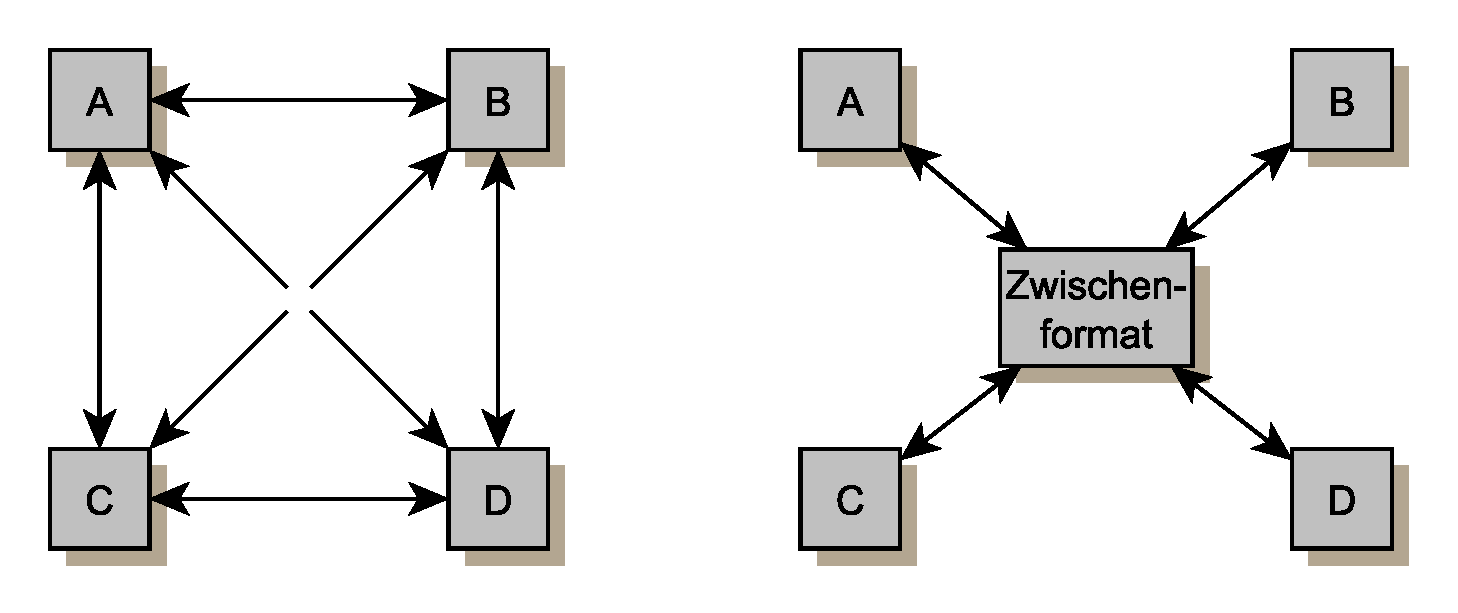
\includegraphics[
        width=0.7\textwidth,
        keepaspectratio=true
    ]{assets/images/interlingua_vs_allvsall}
    \caption{Komplexität ohne und mit dem Einsatz eines Zwischenformats - Originalbild: \cite{Uschold1996a}}
    \label{fig:interlingua_vs_all}
\end{figure}

Eine elegantere Methode für die Lösung dieses Problems, welche die Anzahl zu implementierender Konverter in Grenzen halten kann, wäre die Einführung eines Zwischenformates (auch Inter-Lingua, in Abbildung \ref{fig:lesen_von_beitrag_und_convertieren} als \enquote{IM Format} bezeichnet) \cite[S.\,9]{Uschold1996a}. Geht man davon aus, dass die Daten aller Webseiten nur in dieses Zwischenformat geschrieben und aus diesem gelesen werden müssen, würde sich der Aufwand auf maximal zwei Konverter je Webseite reduzieren. Für eine beliebige Anzahl Webseiten wären also $ n_{k2} = n_{ws} * 2 $ Konverter nötig. Nachteile hätte dieser Ansatz nur für $ n_{ws} = 2 $ und $ n_{ws}=3$ , da in diesen Fällen mehr beziehungsweise gleich viele Konverter gegenüber der ersten Methode erforderlich wären. Erhöht man die Anzahl Webseiten jedoch nur geringfügig, sinkt die Menge an Konvertern sichtbar. Für $ n_{ws} = 4 $ wären es $ n_{k2} = 8 $ statt $ n_{k1} = 12 $ (siehe Abbildung \ref{fig:interlingua_vs_all}) und für $ n_{ws} = 5 $ ergibt sich $ n_{k2} = 10 $ statt $ n_{k1} = 20 $ Konvertern. Gleichzeitig können so syntaktische Unterschiede in den einzelnen Formaten angeglichen werden, was sie leichter handhabbar macht. 

\begin{figure}[ht]
    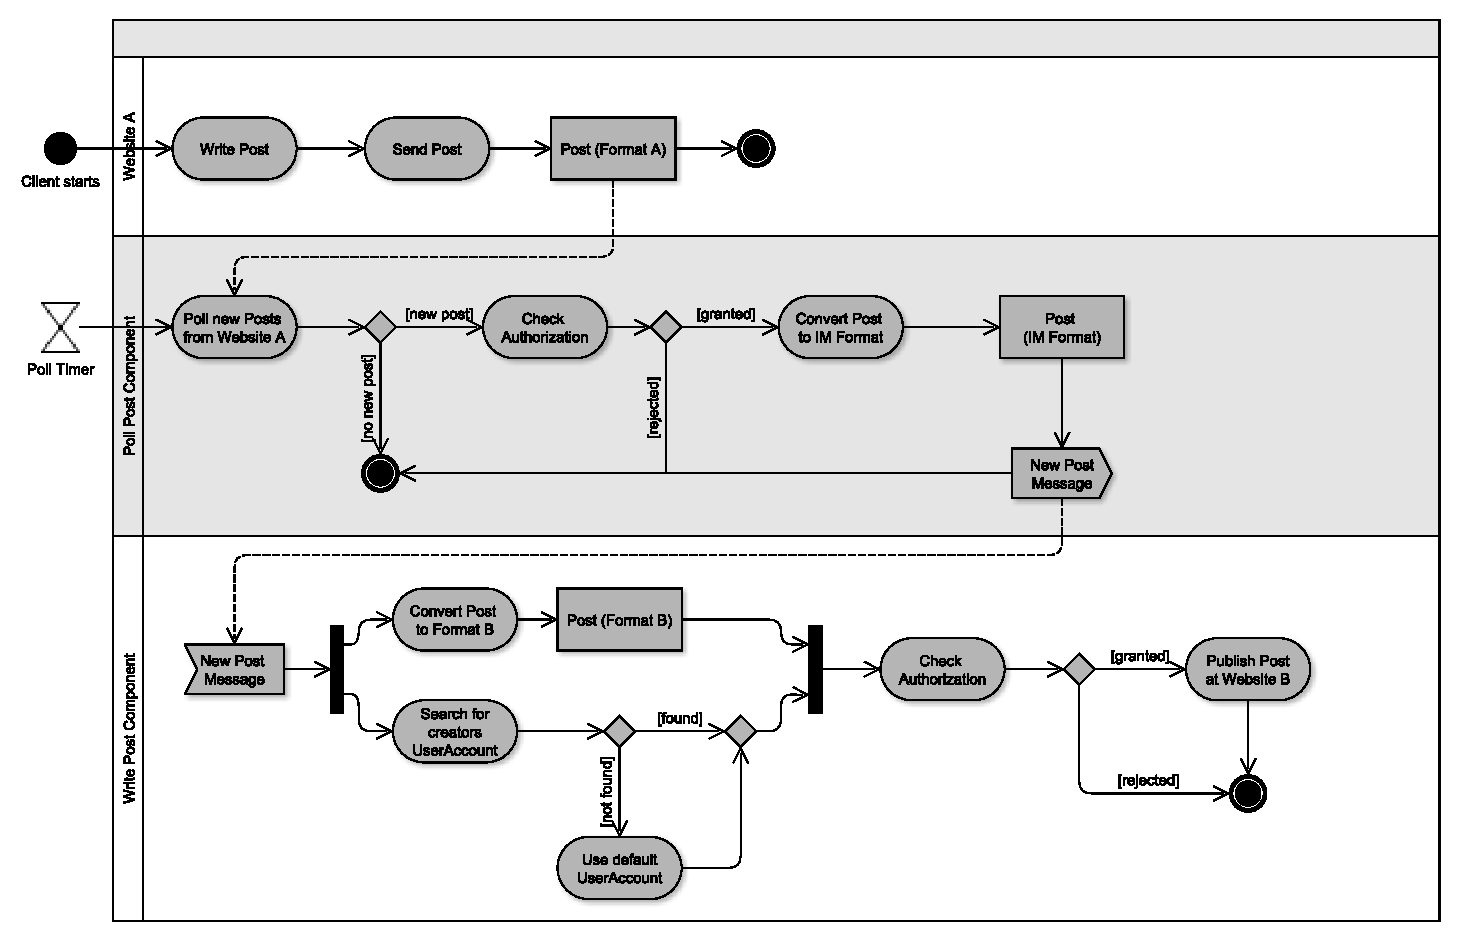
\includegraphics[
        width=\textwidth,
        keepaspectratio=true,
        clip=true,
        trim= 0 193 0 113
    ]{assets/images/activitydiagram_post_as_user_check_authorization.pdf}
    \caption{Lesen des erstellten Beitrags und konvertieren in das Zwischenformat.}
% section beiträge_von_solzialen_netzwerk_a_lesen (end)
    \label{fig:lesen_von_beitrag_und_convertieren}
\end{figure}

Bei der automatischen Sammlung von benutzergenerierten Inhalten stellt sich immer die Frage der Privatsphäre. Nicht jeder möchte, dass vielleicht sensible Informationen von ihnen weitergegeben werden. Aus diesem Grund ist die Einführung eines Mechanismus sinnvoll mit dem ein Benutzer das Lesen seiner Beiträge komplett erlaubt oder auf bestimmte Seiten, Foren oder nur für einzelne Threads beschränkt \cite{Bojars2011}. Sollte eine solche Erlaubnis nicht vorliegen, wird der gelesene Beitrag verworfen.

Da das Eintreffen neuer Beitrage nicht vorhersagbar ist, ist es angebracht beim Synchronisieren das Lesen und Schreiben zeitlich zu entkoppeln. Eine der weit verbreitetsten Techniken dazu ist das Versenden von Nachrichten über einen Nachrichtenkanal den die schreibende Komponente nach neuen Beiträgen abhört. Diesen Kanal können mehrere Gleichzeitig abhören und stellen so eine gute Flexibilität sicher. 

% subsection beiträge_lesen_und_konvertieren (end)

\subsection{Beiträge in eine andere Webseite schreiben} % (fold)
\label{sub:beiträge_in_eine_andere_webseite_schreiben}


Empfängt nun eine Komponente, die für das Schreiben zuständig ist, eine Nachricht von einen neuen Beitrags der Webseite A ist der Ablauf ähnlich wie beim Lesen nur in umgekehrter Reihenfolge (Siehe Abbildung \ref{fig:konvertieren_formatb_und_schreiben} links, oberer Ablauf). Der neue Beitrag wird vor dem Schreiben aus dem Zwischenformat in das Format B konvertiert. Da bei einer Synchronisation vom Vorteil wäre, wenn der synchronisierte Beitrag so aussehen würde, als hätte ihn der original Autor geschrieben. Hierzu muss das System Zugriff auf die Benutzerkonto haben und diese in einer Datenbank verwalten. Dort kann dann nach einen passenden Benutzerkonto des Autors gesucht und dieses dann zum Schreiben verwendet werden. Steht ein solches Benutzerkonto nicht zur Verfügung, ist das Ausweichen auf ein vorgegebenes Benutzerkonto hilfreich. Manche Benutzer sind vielleicht damit einverstanden, dass ihre Beiträge weitergegeben werden, aber nicht dass andere Programme automatisch in ihren Namen Beiträge schreiben. Deswegen ist wichtig davor noch einmal zu prüfen, ob eine entsprechende Erlaubnis gegen wurde. Sind alle Voraussetzungen gegeben, kann der Beitrag über das ausgewählte Benutzerkonto auf die Webseite B geschrieben werden.

\begin{figure}[ht]
     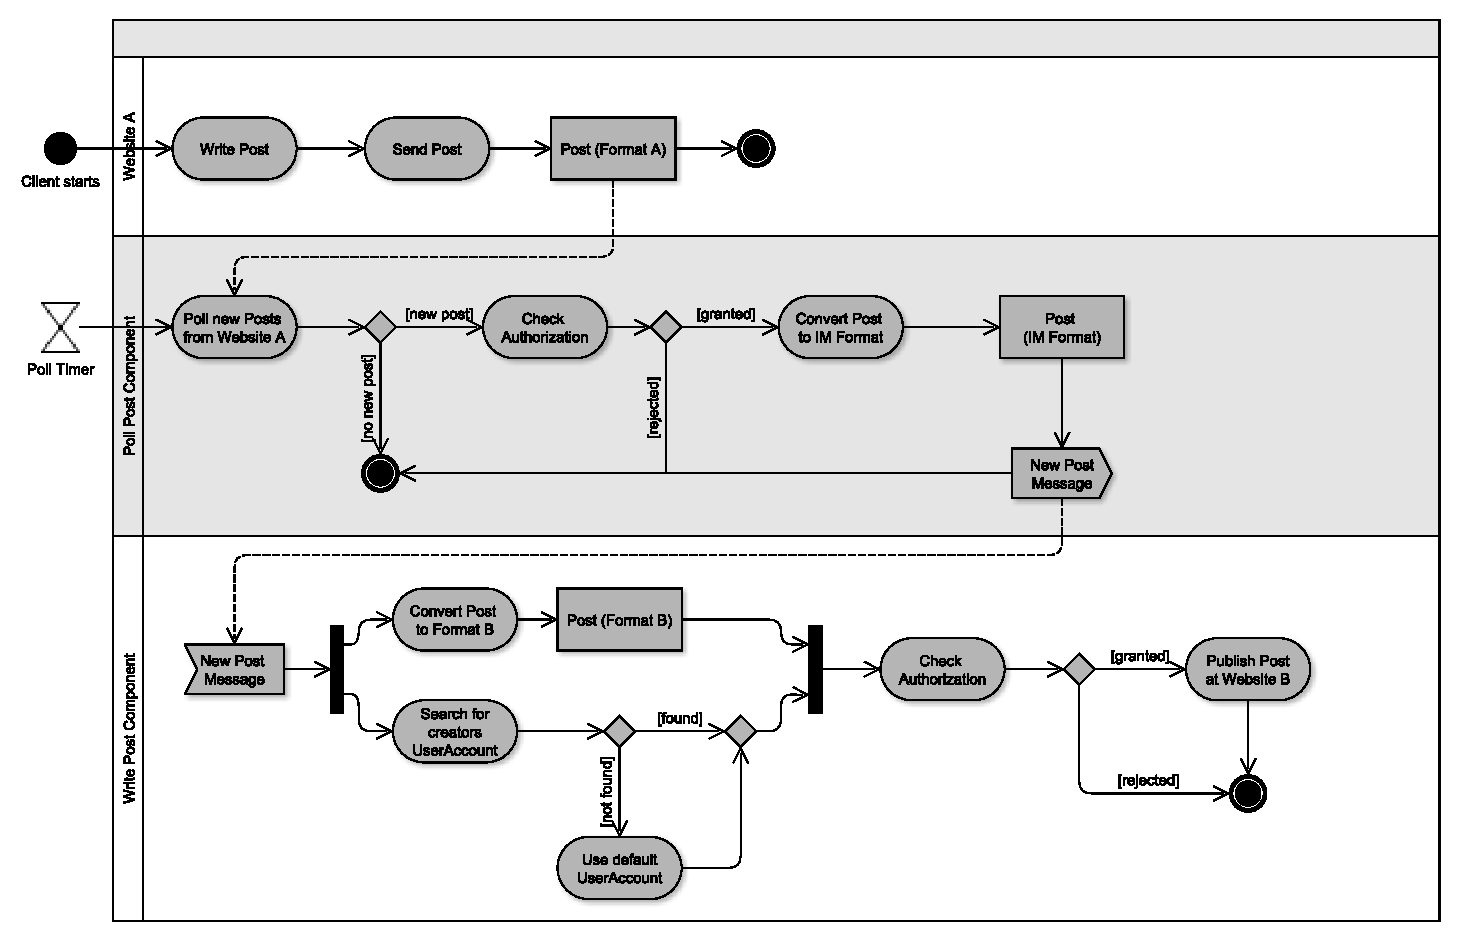
\includegraphics[
        width=\textwidth,
        keepaspectratio=true,
        clip=true,
        trim= 0 0 0 257
    ]{assets/images/activitydiagram_post_as_user_check_authorization.pdf}
    \caption{Konvertierten des Beitrags in das Format B und schreiben n das soziale Netzwerk B}
    \label{fig:konvertieren_formatb_und_schreiben}
\end{figure}

% subsection beiträge_in_eine_andere_webseite_schreiben (end)

\section{Identifizierung der Komponenten} % (fold)
\label{sec:identifizierung_der_komponenten}

Anhand dieses kurzen Ablaufbeispiels kann man einige Komponenten ablesen, aus denen das neue System auf jeden Fall bestehen beziehungsweise enthalten muss und welche ergänzend dazu Wünschenswert wären:

\begin{itemize} 
    \item Eine Komponente muss Daten von einen Webseite über deren öffentlicher API in das System einlesen und diese in ein geeignetes Zwischenformat konvertieren können.
    \item Es muss ein passendes Nachrichtensystem zum Entkoppeln von Lesen und Schreiben gewählt und/oder erstellt werden.
    \item Eine weitere Komponente nimmt Beiträte im Zwischenformat entgegen, konvertiert diese in das Format des entsprechenden Netzwerkes und schreibt diese dorthin.
    \item Um stellvertretend für einen Benutzer schreiben zu können, muss es möglich sein nach dem Konto eines Benutzer zu einer bestimmten Webseite suchen zu können.
    \item Um die Privatsphäre der Benutzer zu wahren, wäre eine Mechanismus zum festlegen von Zugriffsrechen sinnvoll.
\end{itemize}   

% section identifizierung_der_komponenten (end)

\section{Wahl vorhandener Techniken} % (fold)
\label{sec:wahl_vorhandener_techniken}

\todo[inline]{vielleicht doch eher an den Anfang von "Eigener Ansatz"!?}

\subsection{Welches Zwischenformat?} % (fold)
\label{sub:welches_zwischenformat}

Ein passendes Zwischenformat wurde im Kapitel \enquote{\ref{cha:grundlagen}} mit SIOC beziehungsweise die Kombination aus SIOC und FOAF bereits vorgestellt. Damit ist es nicht nur möglich einzelne Beiträge plattformunabhängig zu speichern, sondern es kann auch die Struktur der Plattform als auch der Benutzer mit eingebunden werden. Auch können Maschinen aus den RDF-Daten einfach Wissen für neue, hilfreiche Informationen ableiten. Doch warum sollte man auf RDF und Ontologien setzen anstatt etwas eigenes zu Entwickeln wie auf Basis des weitverbreiteten und vielseitigen XML Formats?

Hier gibt es mehrere Vorteile, warum man RDF einer mit XML-Schema definierten XML-Datei vorziehen sollte. XML hat das Problem, dass die selbe Aussage auf verschiedene Art repräsentiert werden kann. Listing \ref{lst:xml_vs_rdf_multiple_rep} zeigt ein Beispiel für die Repräsentation der Aussage \enquote{Max Hiwi ist der Autor des Beitrags mit der ID 42} in XML.

\begin{lstlisting}[
    language=XML,
    caption={XML: Unterschiedliche Syntax, gleiche Semantik }\label{lst:xml_vs_rdf_multiple_rep},
    captionpos=t]
    <post>
        <id>42</id>
        <author>Max Hiwi</author>
    </post>

    <post id="42">
        <author>Max Hiwi</author>
    </post>

    <post id="42" author="Max Hiwi" />
\end{lstlisting}

Alle drei XML-Elemente beschreiben die selbe Aussage, aber auf unterschiedliche Art und Weise. Für einen Menschen haben diese drei Schreibweisen die selbe Aussage, für eine Maschine ist dies aber nicht mehr ganz so offensichtlich. Auch kann nicht die Bedeutung der einzelnen Element und Tags von Maschinen erfasst werde. Dies muss der Programmierer erledigen.Zusätzlich erschweren diese Unterschiedlichen Strukturen das ausführen von Abfragen auf diesen Daten, da ein Mapping zwischen einer logischen Abfrage und den Daten nicht eindeutig erfolgen kann (vgl. \cite[s.\,41]{Schroder2003a}).

% subsection welches_zwischenformat (end)

\subsection{Welches Nachrichtensystem?} % (fold)
\label{sub:welches_nachrichtensystem}

\subsubsection{JMS} % (fold)
\label{ssub:analyse_jms}
\begin{itemize}
    \item zum reinen verschicken ausreichend
    \item fast alles muss selber gemacht werden.
\end{itemize}
    
\subsubsection{Apache Camel} % (fold)
\label{ssub:analyse_apache_camel}
    \begin{itemize}
        \item erweitern der "Pipeline" z.B. mit Filtern einfach möglich
    \end{itemize}

\subsubsection{JMS + Apache Camel} % (fold)
\label{ssub:analyse_jms_apache_camel}

\begin{itemize}
    \item gute kombination -> durable subscriber
\end{itemize}

% subsubsection analyse_jms_apache_camel (end)

% subsubsection analyse_apache_camel (end)

% subsubsection analyse_jms (end)

% subsection welches_nachrichtensystem (end)

% section wahl_vorhandener_techniken (end)

% chapter analyse (end)
		%!TEX root = ../thesis.tex

\chapter{Eigener Ansatz: Social Online Community Connectors (SOCC)} % (fold)
\label{cha:eigener_ansatz_social_online_community_connectors_socc_}

Aufbauend auf den in Kapitel \ref{cha:analyse} identifizierten Komponenten und Wahl der für ein System zur Synchronisation von Beiträgen passenden Techniken, soll nun der als \emph{Social Online Community Connectors} (SOCC) benannter Ansatz vorgestellt werden. Den Aufbau von SOCC ist in Abbildung \ref{fig:uebersicht_socc} zu sehen. Ein \emph{Connector} von SOCC dient dabei als Schnittstelle zwischen den Datenformat der Plattform für die er implementiert wurde und dem SIOC-Format. SOCC stützt sich dabei auf die Prinzipien für die Verbindung von Daten im Web von Tim Berners-Lee (siehe \cite{Berners-Lee2009}):

\begin{description}
    \item[\enquote{Use URIs as names for things}:] Ressourcen wie Seiten, Foren, Threads und Beiträge sollten immer durch eine URI benannt werden.

    \item[\enquote{Use HTTP URIs so that people can look up those names}:] Die verwendeten URIs sollten einer Adresse im Web entsprechen, um auf die dahinter liegenden Daten zugreifen zu können.

    \item[\enquote{When someone looks up a URI, provide useful information, using the standards (RDF*, SPARQL)}:] Die Daten sollten in einen Standard für das Semantic Web formatiert werden. Wie schon erwähnt setzt SOCC dazu auf RDF und darauf aufbauenden Ontologien wie FOAF und SIOC. Dadurch können zum Beispiel andere Anwendungen mit Anfragen in SPARQL\footnote{\url{http://www.w3.org/TR/sparql11-overview}} nach Beiträgen suchen.

    \item[\enquote{Include links to other URIs. so that they can discover more things.}:] Nicht nur die Struktur eine Diskussion kann über Links rekonstruiert werden, auch der Gewinnen zusätzlicher Informationen ist so möglich. Beiträge können auf Lernmaterialien wie Folien oder Videos verweisen oder über das FOAF-Profil eines Autor können weitere Beiträge von ihm gefunden werden. 
\end{description}

URIs sind also das wichtigste Element mit denen SOCC arbeitet. Soll zum Beispiel eine Diskussion synchronisiert werden, muss einem Connector die URI übergeben werden, hinter der sich die Daten befinden. Ein Connector ist nur für eine einzige Plattform zuständig. Aber eine Plattform kann über mehrere Connectoren angesprochen werden.

\begin{figure}[ht]
    \centering
    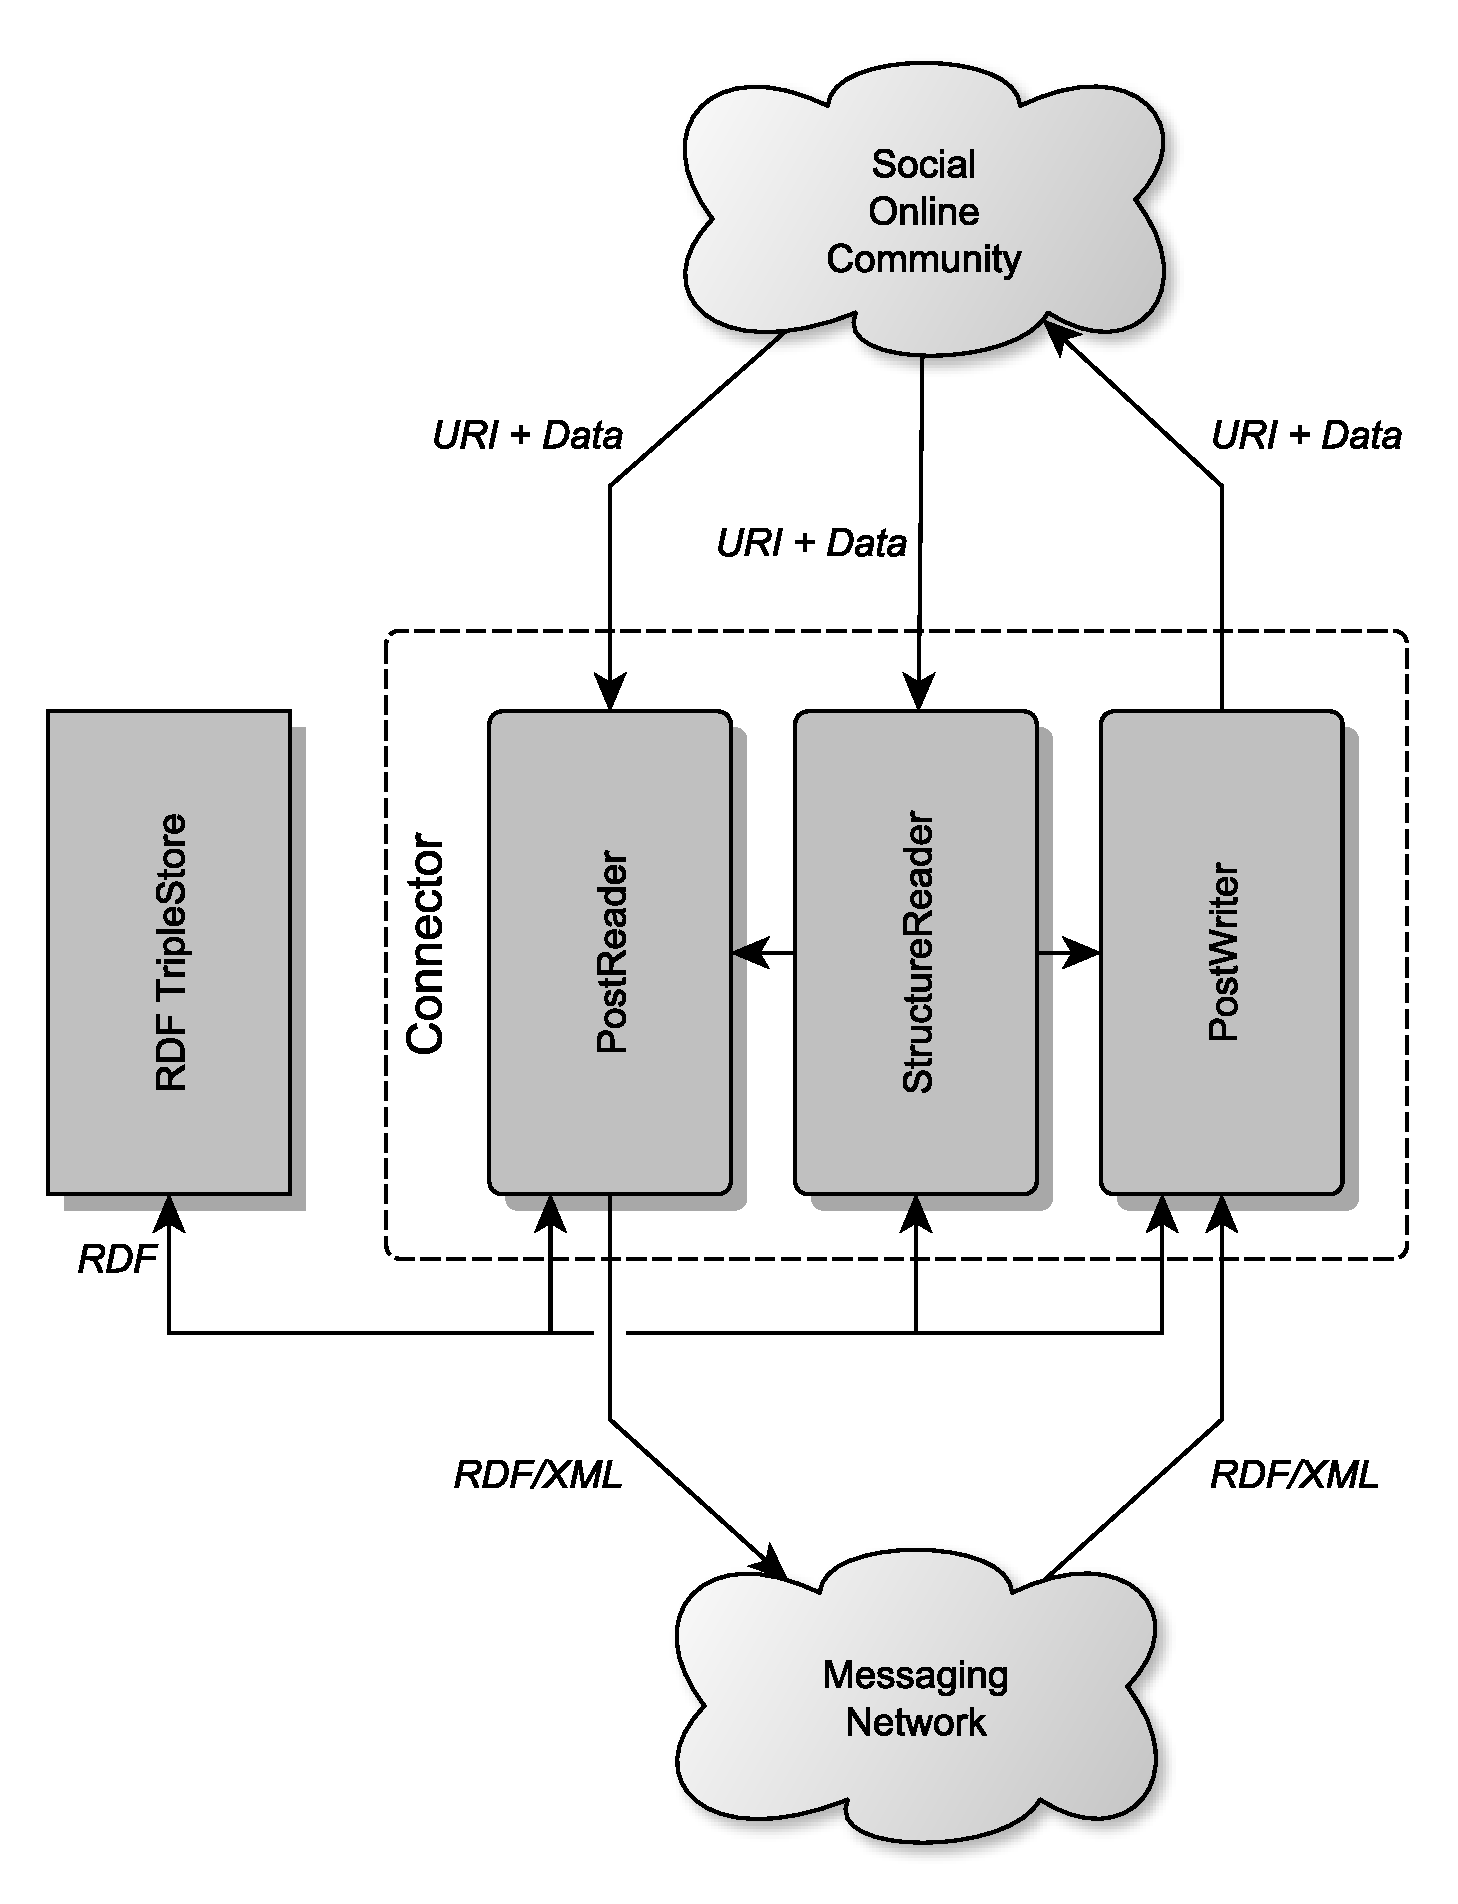
\includegraphics[
        width=0.5\textwidth,
        keepaspectratio=true]
    {assets/images/socc_connector_overview}
    \caption{Übersicht der Komponenten der SOCC}
    \label{fig:uebersicht_socc}
\end{figure}

Intern besteht ein Connector aus drei Komponenten die zum Einen für das Lesen (\emph{PostReader}) und Schreiben (\emph{PostWriter}) von Beiträgen verwendet werden, zum Andren aus einen \emph{StructureReader} der für das Auslesen der Struktur der Plattform verantwortlich ist. Eine genaue Beschreibung dieser Komponenten folgt in Abschnitt \ref{sec:design_eines_connectors}.

Jeder Connector hat Zugriff auf eine als \emph{Triplestore} bezeichnete Datenbank in der RDF-Triple gespeichert und mit SPARQL abgefragt werden können. Der Connector benutzt diesen Triplesore als Speicher in dem seine Konfigurationsdaten lagern, aber auch für zusätzliche Daten die er von Außerhalb benötigt. Er wird aber auch benutzt um Daten zu speichern, die während des Betriebes anfallen, da sie so irgendwann wieder verwendet werden können ohne sie erneut aus der von der Plattform laden zu müssen. Zum Beispiel die Daten über die Struktur der verwendeten Plattform, die sich selten ändert.

Die Beiträge werden dann zwischen den einzelnen Connectoren über ein Nachrichtennetzwerk auf der Basis von Apache Camel ausgetauscht. Die Beschreibung dieser als \emph{SOCC-Camel} bezeichneten Komponnente erfolgt in Abschnitt \ref{sec:socc_camel}.

% section datenformat (end)

\section{Konfiguration} % (fold)
\label{sec:konfiguration}

Damit ein Connector funktionieren kann, muss er von außen Informationen bekommen, welche er zum Betrieb braucht. Die sind zum Beispiel Informationen zu Benutzerkonten oder Parameter für die verwendete API. Da einige dieser Informationen nicht nur von einen Connector benutzt werden, ist es sinnvoll diese zusammen an einen Ort zu speichern und wiederverwenden zu können. Wofür der oben angesprochene Triplestore verwendet wird. Die wichtigsten Informationen für die Konfiguration der Connectoren stellen die Benutzerkonten dar. Sie enthalten unter anderem die Informationen, um Zugriff auf die Operationen der einzelnen APIs zu erhalten. Da die Benutzerkonten, wie später im Abschnitt \ref{sub:benutzerdaten} beschrieben, im FOAF-Format gespeichert werden, stellt es sich als Vorteil heraus die übrigen Informationen ebenfalls dort zu speichern und mit den schon vorhandenen zu verbinden. 

Aus diesem Grund wurde für Konfiguration eines Connectors die \emph{SOCC Connector Config Ontology} entwickelt. Diese Ontologie ist sehr einfach gehalten und baut auf schon vorhandenen Ontologien auf. Zusätzlich musste die SIOC-Ontologie so erweitert werden, dass die Integration von Authentifizierungs- und Autorisierungsinformationen möglich war. 

\subsection{SOCC Connector Config Ontologie} % (fold)
\label{sub:connector_config_ontologie}

Der Aufbau der SOCC Connector Config Ontologie (RDF-Präfix \texttt{ccfg:}) ist in der Abbildung \ref{fig:uebersicht_conector_cfg} zu sehen. Die Konfigurationsdaten für einen Connector werden dabei durch die Klasse \texttt{ccfg:ConnectorConfig} modelliert. Diese Klasse enthält dann die folgenden Eigenschaften für den Connector.

\begin{figure}[ht]
    \centering
    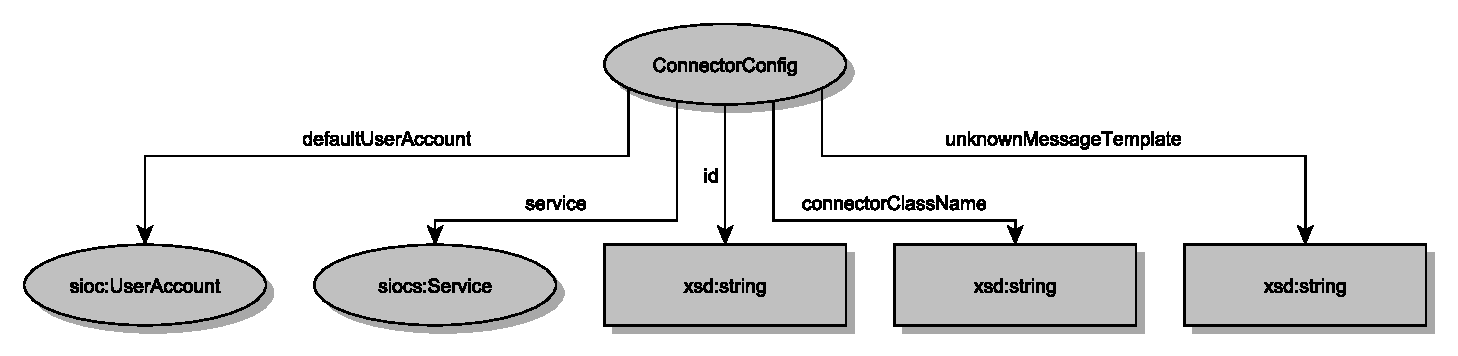
\includegraphics[
        width=\textwidth,
        keepaspectratio=true
    ]{assets/images/connector_config_ontology}
    \caption{Schema der SOCC Connector Config Ontology}
    \label{fig:uebersicht_conector_cfg}
\end{figure}

Jeder Connector erhält einen eindeutigen \texttt{ccfg:id} zugewiesen, um jeden Connector später eindeutig identifizieren zu können. Die Eigenschaft \texttt{ccfg:connectorClassName} beschreibt den vollständigen Java-Klassennamen des beschriebenen Connectors. Diese wird für das Laden der richtigen Implementierung benötigt. Manchmal kann es passieren, dass keine passendes Benutzerkonto zum Schreiben eins Beitrags gefunden werden kann. Dadurch es es wünschenswert solche Beiträte dahingegen zu verändern, dass eine Verweis auf den original Autor und vielleicht wo der Beitrag gemacht wurde vorhanden ist. Durch die Eigenschaft \texttt{ccfg:unknownMessageTemplate} kann eine Vorlage für das Aussehen des Verweises definiert werden. Innerhalb dieser Vorlage stehen einige Variablen in der Form \enquote{\texttt{\{varName\}}} zur Verfügung, wobei \enquote{varName} durch den Namen der entsprechenden Variable zu ersetzen ist. Welche Variablen alle vorhanden sind und mit welchen Werten diese ersetzt werden, ist in Tabelle \ref{tbl:unknown_message_template_vars} zu sehen. 

\begin{table}[ht]
    \caption{Variablennamen und Ersetzung innerhalb von \texttt{ccfg:unknownMessageTemplate} }
    \centering
    \begin{tabular}{l|l}
        \textbf{varName} & \textbf{Ersetzt durch} \\
        \hline
        \texttt{message} & Original Beitrag \\
        \texttt{sourceUri} & URI des original Beitrags \\
        \texttt{connectorId}  & ID des aktuellen Connectors \\
        \texttt{serviceName}  & Name des vom Connector verwendeten Service \\
        \texttt{creationDate} & Erstelldatum des Beitrags (falls bekannt) \\
        \texttt{authorName}   & Name des Autors (falls bekannt)          
    \end{tabular}
    \label{tbl:unknown_message_template_vars}
\end{table}

Für die Nutzung einiger APIs müssen zusätzlich bestimmte Parameter angegeben werden. Dies könnte zum Beispiel die genau Adresse des Dienstes sein. Hierzu wird auf das \emph{SIOC Services Modul} zurückgegriffen. Diese stellt eine Klasse \texttt{sioc:Service} zur Verfügung und über die Eigenschaft \texttt{ccfg:service} kann eine solche Servicebeschreibung einen Connector zugewiesen werden. Der genaue Aufbau eines solchen Services wird im Abschnitt \ref{sub:services} dargestellt. Die letzte Information für die Konfiguration eins Connectors ist eine Standardbenutzer (Im Folgenden Defaultuser genannt) und wird mit der Eigenschaft \texttt{ccfg:defaultUserAccount} festgelegt. Dieser Defaultuser erfüllt im Großen und Ganzen zwei Aufgaben. Als Erstes wird er für lesende Zugriffe der API auf die verwendete Plattform genutzt. Hierzu ist ein einzelnes Benutzerkonto vollkommen ausreichend, da nur die gelesenen Daten wichtig sind und nicht von welchen Konto sie kommen. Es sollte aber ein Konto mit weitreichenden Befugnissen sein, um möglichst viel Daten lesen zu können.Die zweite Aufgabe bezieht sich auf das stellvertretende Schreiben einzelner Benutzer. Nicht immer werden die dazu notwendigen Daten von den Benutzer zur Verfügung gestellt oder sind unbekannt. In diesem Fall wird der Defaultuser genutzt und der Inhalt des Beitrags in die Form der mit der Eigenschaft \texttt{\texttt{ccfg:unknownMessageTemplate}} festgelegten Vorlage konvertiert. 

% subsubsection connector_config_ontology (end)

\subsection{Services} % (fold)
\label{sub:services}

Wie eben schon beschrieben, existiert für SIOC ein Modul zur einfachen Modellierung von Diensten auf semantischer Ebene: Das SIOC Services Module (RDF-Präfix \texttt{siocs:}). Kernstück dieses Moduls ist die Klasse \texttt{siocs:Service}, wie auf Abbildung \ref{fig:uebersicht_sioc_services} zu sehen ist. Mit dieser Klasse kann durch eine Hand voll Eigenschaften ein Service beschrieben werden. Für diese Arbeit ist davon die wichtigste Eigenschaft \texttt{siocs:service\_endpoint}. Durch diese kann die Adresse festgelegt werden, unter dem ein Service erreichbar ist. Gerade bei Plattformen die nicht an eine feste Adresse (Foren, Blogs, $\dots$) gebunden sind, ist diese Angabe unerlässlich. Die Eigenschaften \texttt{siocs:has\_service} und \texttt{siocs:service\_of} sind ideal zur Verbindung von einzelnen \texttt{sioc:UserAccount}s mit einem Service. Diese Verbindung hilft dabei für das stellvertretende Schreiben von Beiträgen schnell die passenden Benutzerdaten zu finden. Ebenfalls nützlich ist \texttt{siocs:max\_results}. Manche Dienste erlauben es nur eine maximale Anzahl an Ergebnissen pro Aufruf zurückgeben zu lassen. Da sich diese Anzahl über die Zeit ändern kann ist es nicht sinnvoll diese fest im Programm festzulegen. Für SOCC weniger interessant aber der Vollständigkeit halber seien noch \texttt{siocs:service\_protocol} zum Angeben des verwendeten Übertragungsprotokolls REST, SOAP, $\dots$) und \texttt{siocs:service\_definition} mit dem auf eine weiterführende Definition verwiesen werden kann erwähnt. 

\begin{figure}[ht]
    \centering
    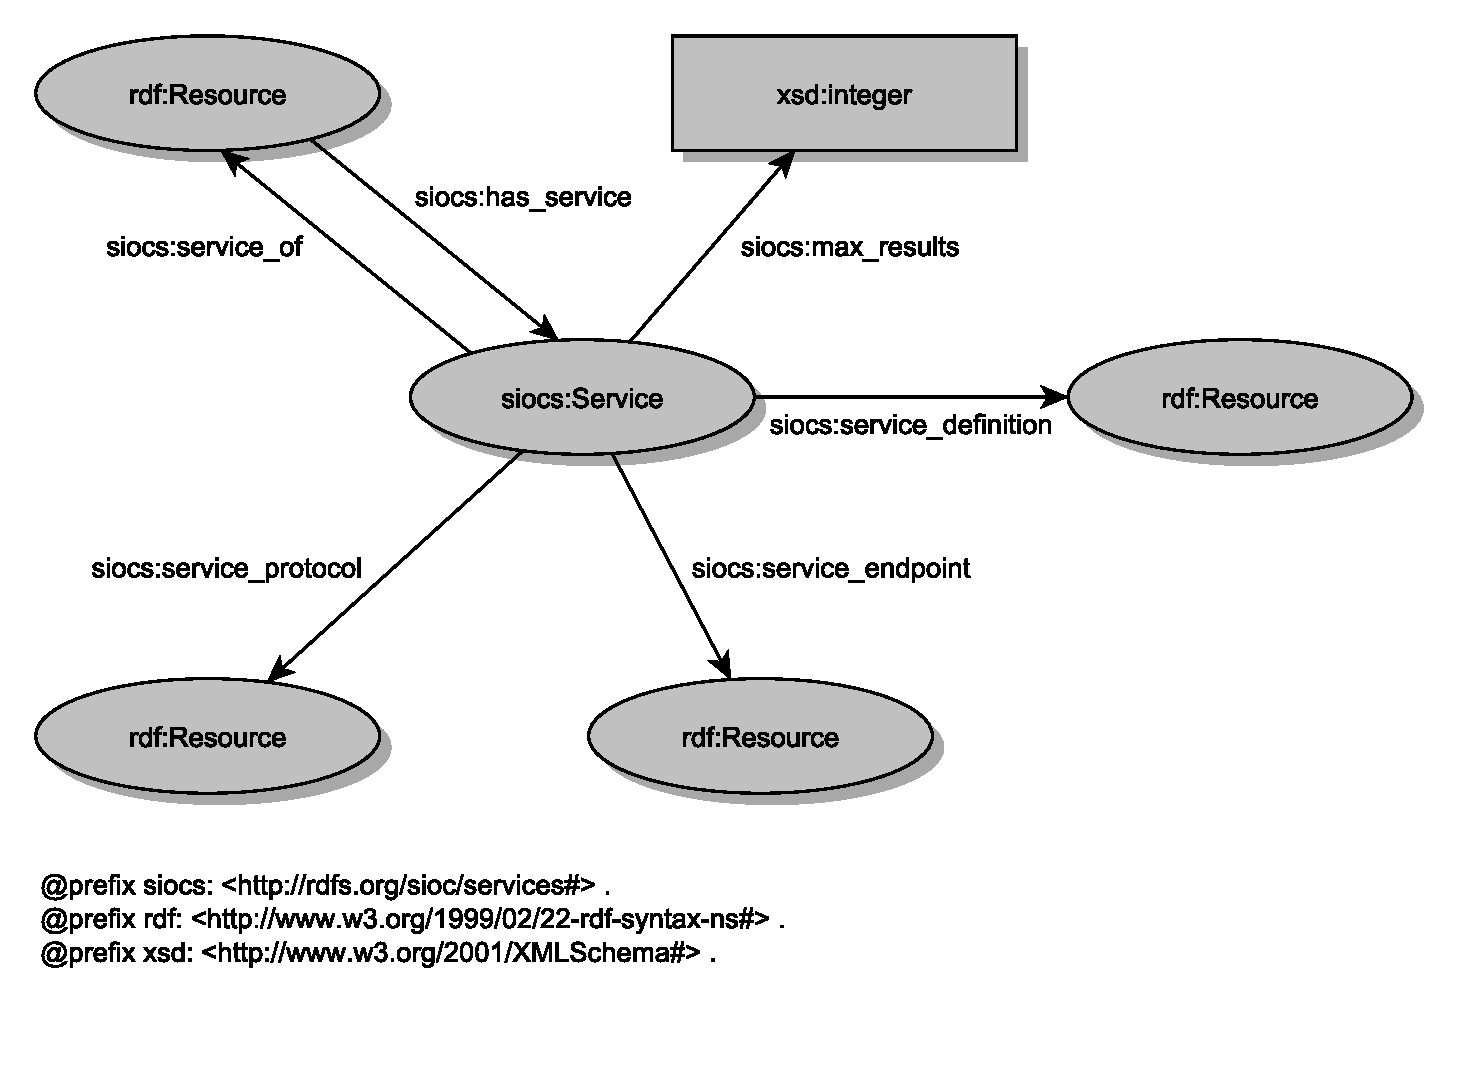
\includegraphics[
        width=\textwidth,
        keepaspectratio=true
    ]{assets/images/sioc_services_ontology}
    \caption{SIOC Services Module}
    \label{fig:uebersicht_sioc_services}
\end{figure}

% subsection services (end)

\subsection{Benutzerdaten} % (fold)
\label{sub:benutzerdaten}

Soll ein Beitrag eines Benutzers von Google+ nach Facebook synchronisiert werden und es so aussehen, als hat er diesen Beitrag selbst auf Facebook geschrieben, sind gute Kenntnisse über alle Benutzerkonten dieser einen Person notwendig. Als erstes muss die Existenz dieser Person dem System bekannt sein. Hierzu kann diese durch die Klasse \texttt{foaf:Person} aus der FOAF Ontologie dargestellt werden. Für ein einzelnes Benutzerkonto wurde in SIOC die Klasse \texttt{sioc:UserAccount} definiert. Da \texttt{sioc:UserAccount} eine Unterklasse von \texttt{OnlineAccount} aus FOAF ist, kann diese über die Eigenschaft \texttt{foaf:account} beziehungsweise \texttt{sioc:account\_of} mit einer Person verbunden werden. Ebenso ist es wichtig zu wissen zu welchen Plattform ein Benutzerkonto gehört. Deshalb wird der \texttt{sioc:UserAccount} mit einem Objekt der Klasse \texttt{siocs:Service} über die Eigenschaft \texttt{siocs:has\_service}/\texttt{siocs:service\_of} zusammengebracht. Diese Verbindung ist für manche APIs besonders bedeutend, da in dem Serviceobjekt relevante Daten für den Zugriff darauf enthalten sind. Nun kann es vorkommen, dass eine Person mehrere Benutzerkonten für private und geschäftliche Dinge besitzt. Um nicht private Beiträge auf Webseite A mit dem geschäftlichen Benutzerkonto auf Webseite B zu schreiben, muss ein Mapping zwischen den verschiedenen Benutzerkonten festgelegt werden. Dieses Mapping kann über ein in der \enquote{\nameref{sec:anhang_socc_connector_config_ontologie}} definierte Eigenschaft \texttt{ccfg:mapped\_to} realisiert werden. Diese Eigenschaft ist symmetrisch, also falls Benutzerkonto A mit Benutzerkonto B über \texttt{mapped\_to} verbunden ist, dann gilt dies ebenfalls für B mit A. Abbildung \ref{fig:usermanagement} zeigt den Zusammenhang zwischen der Klasse \texttt{foaf:Person}, \texttt{sioc:UserAccount} und \texttt{siocs:Service} sowie der Eigenschaft \texttt{ccfg:mapped\_to} noch einmal graphisch an einem Beispiel.

\begin{figure}[ht]
    \centering
    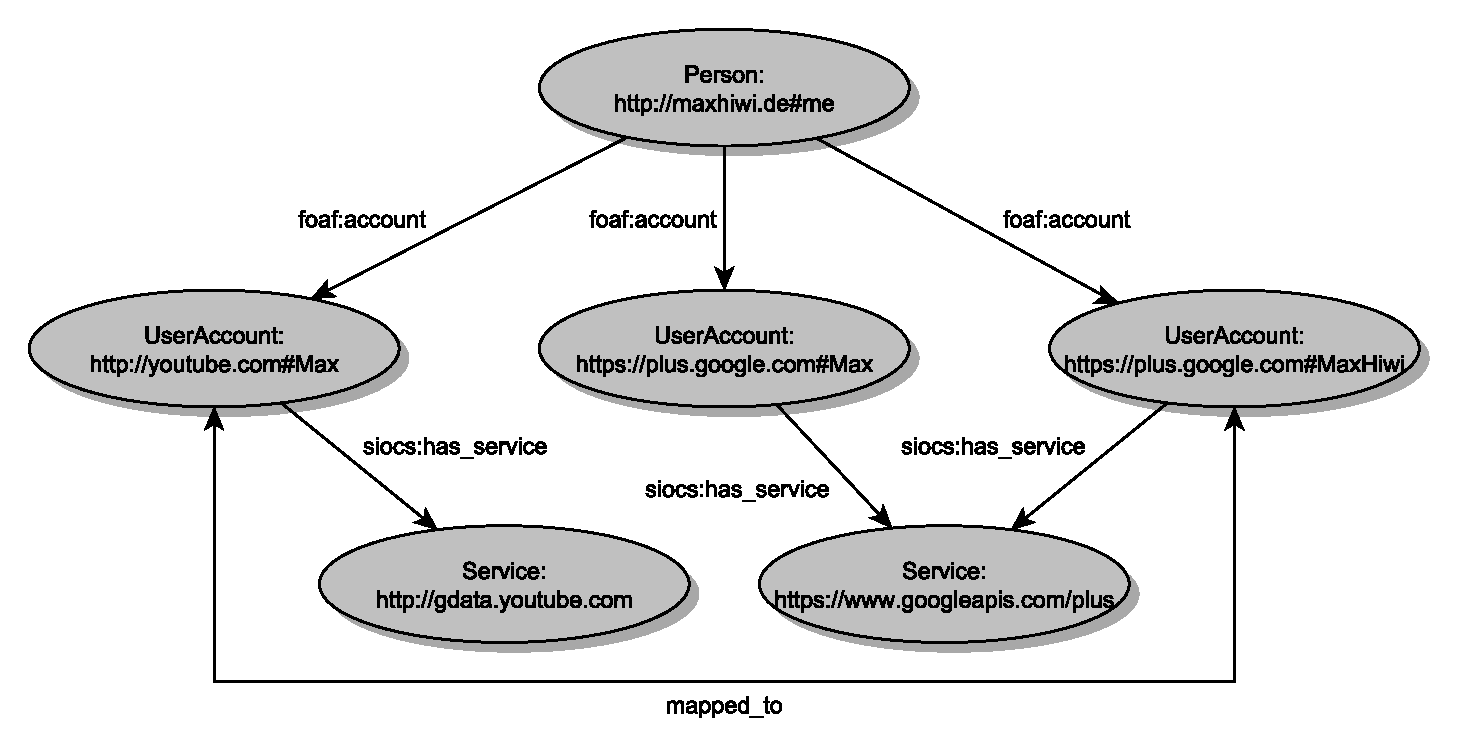
\includegraphics[
        width=\textwidth,
        keepaspectratio=true,]
    {assets/images/usermanagement}
    \caption{Zusammenhang von Person, UserAccount und Service. Die inversen Eigenschaften \texttt{sioc:account\_of} und \texttt{siocs:service\_of} wurden zu einer besseren Übersicht weggelassen}
    \label{fig:usermanagement}
\end{figure}

% subsubsection benutzerdaten (end)

\subsection{Authentifizierung} % (fold)
\label{sub:authentifizierung}

Die Ontologien FOAF und SIOC sind hervorragend für die Abbildung von sozialen Netzwerken und Diskussionen geeignet, jedoch ist es mit ihnen nicht möglich Daten zur Authentifizierung (Feststellen ob jemand der ist, den er vorgibt zu sein) zu speichern. Wegen dem Schutz der Privatsphäre ist dies verständlich, jedoch um stellvertretend für einen Benutzer Beiträge zu schreiben, ist es wichtig Zugriff auf diese Daten zuhaben und sie einem Benutzerkonto zuordnen zu können. Zuerst muss dazu aber festgestellt werden, welche verschiedenen Mechanismen es zum Anmelden an ein solches Konto existieren.

\begin{description}
    \item[Benutzername/Passwort] ist wohl eine der ersten und häufigsten Mechanismen, um den Zugriff sensibler Daten vor Dritten zu schützen. Moodle und Youtube setzen zum Beispiel den Benutzername und Passwort eines angemeldeten Benutzers zu Authentifizierung ein.
    
    \item[OAuth] ist technisch gesehen eher ein Mechanismus zur Autorisierung als zu Authentifizierung. Da es aber auch Informationen enthält die ein Programm zur Authentifizierung von sich gegenüber einer API enthält, wir diese in diesen Abschnitt behandelt.OAuth\footnote{OAuth Webseite: \url{http://oauth.net/}} wird heutzutage hauptsächlich für den zugriff auf webbasierte APIs verwendet. Benutzer können so temporär Programmen den Zugriff auf ihre Daten erlauben und später wieder verbieten. Die aktuelle Version stellt OAuth 2.0 dar und wird in dieser Version von den größten Seitenbetreibern wie Google, Facebook oder Microsoft eingesetzt\footnote{OAuth Versionen im Einsatz: \url{http://en.wikipedia.org/wiki/OAuth\#List\_of\_OAuth\_service\_providers}}. Insgesamt sind für die Nutzung von OAuth vier Parameter wichtig. Für das Programm, dass Zugriff erhalten möchte, sind es die Parameter \emph{client\_id} und \emph{client\_secret} (Siehe \cite{rfc6749}[S.\,8]). Sie weisen das Programm als autorisiert für die Benutzung der API aus. Will man nun eine von OAuth geschützte Funktion nutzen, ist ein sogenannter Accesstoken nötig (Siehe \cite{rfc6749}[S.\,9]). Da dieser Accesstoken in der Regel nur eine bestimmte Zeit gültig ist, wird je nach Implementierung des Standards noch ein Refreshtoken mitgeliefert. Mit diesem Refreshtoken ist das Programm in der Lage ohne Zutun des Benutzers einen abgelaufen Accesstoken wieder zu aktivieren. Dies kann beliebig oft wiederholt werden, bis der Benutzer beide Token für ungültig erklärt. 
    %\todo[inline]{vll. noch OAuth 1.0(a) einbauen}
    
    \item[API Schlüssel] sind eine dritte Möglichkeit Programmen Zugriff auf eine API zu gewähren. Der API Schlüssel entspricht ungefähr einer Kombination von client\_id und client\_secret von OAuth. Dieser Schlüssel schaltet in der Regel nicht den Zugriff auf persönliche Daten von Benutzer frei. Dafür ist noch ein weiterer Mechanismus wie die Verwendung von einem Benutzername und Passwort nötig. Die in Abschnitt \ref{sub:youtube_connector}  beschriebene Google Youtube API hierzu ein gutes Beispiel.
\end{description}

\begin{figure}[ht]
    \centering
    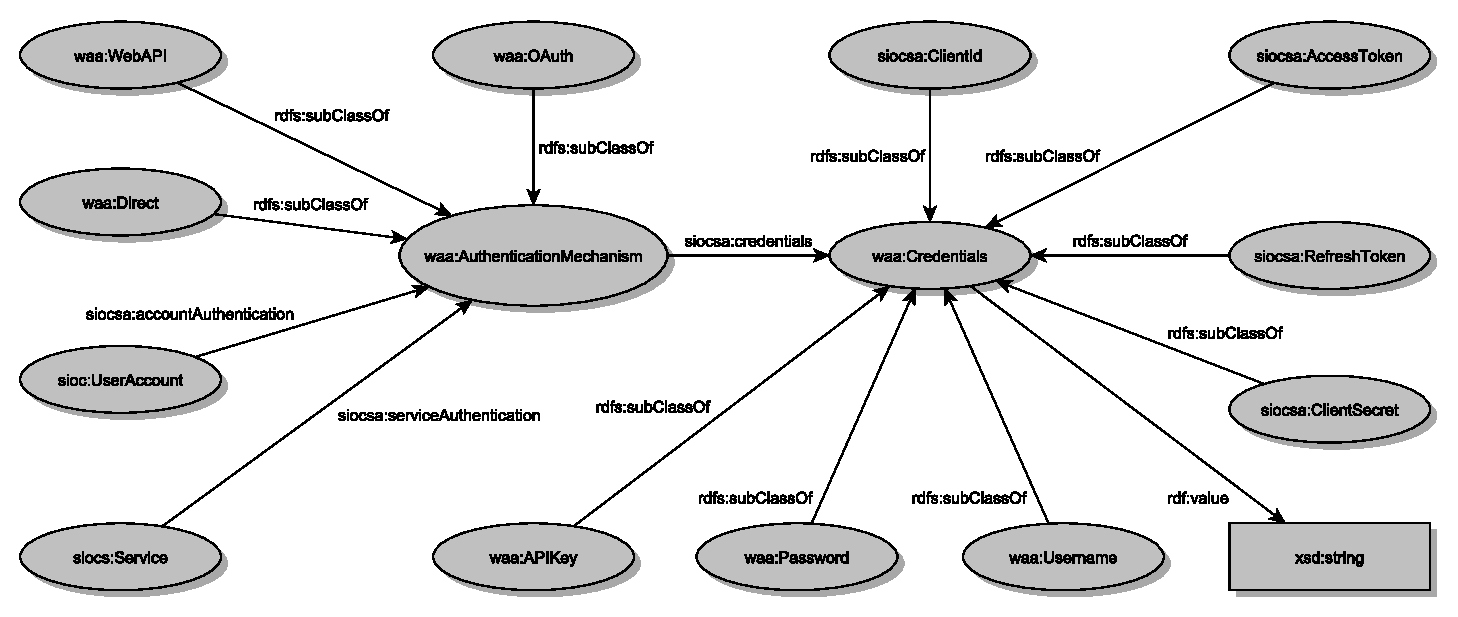
\includegraphics[
        width=\textwidth,
        keepaspectratio=true]
    {assets/images/sioc_services_authentication}
    \caption{SIOC Services Authentication Ontology}
    \label{fig:uebersicht_sioc_services_authentication}
\end{figure}

Neben diesen drei Mechanismen wäre noch der Vollständigkeit halber die HTTP-Authentifizierung zu nennen. Hierbei handelt es ich um eine Form des Benutzername-Passwort-Verfahrens, welches auf dem HTTP Protokoll aufsetzt. Für einfachen Webseiten ist dies ein unkomplizierte Art die Datei vor fremden Zugriffen zu schützten. Für aktuelle öffentliche APIs ist diese Form der Authentifizierung nicht mehr Stand der Technik.

Die Suche nach einer bestehen Ontologie, welche zusammen mit SIOC verwendet werden könnte, gestaltete sich als sehr schwierig. Eine Ausnahme stellt die \emph{Authentication Ontology}\footnote{Authentication Ontology: \url{http://omnivoke.kmi.open.ac.uk/authentication/}} (RDF-Prefix \texttt{waa:}) des \emph{OmniVoke}\footnote{OmniVoke: \url{http://omnivoke.kmi.open.ac.uk/framework/}} Frameworks dar. Die Art der Authentifizierung wird darin durch die Klasse \texttt{waa:AuthenticationMechanism} modelliert. Unterklassen davon für die wichtigsten Mechanismen wie \texttt{waa:OAuth}, \texttt{waa:WebAPI} und Benutzername/Passwort (dort \texttt{waa:Direct} genannt) sind vorhanden. Jedem AuthenticationMechanism Objekt können dann \texttt{waa:Credentials} (engl. für Anmeldedaten) angehängt werden.

Das einzige Manko an dieser Ontologie war das Fehlen von Credentials für OAuth in der Version 2.0. Im einzelnen waren dies Klassen für clien\_id, client\_secret sowie für Access- und Refreshtoken. Um auch diese OAuth Version unterstützen zu können, wurden hierfür die Klassen \texttt{siocsa:ClientId}, \texttt{siocsa:ClientSecret}, \texttt{siocsa:AccessToken} und \texttt{siocsa:RefreshToken} als Unterklassen von \texttt{waa:Credentials} abgeleitet. Als Letztes musste noch eine Verbindung zwischen Authentication Ontology und SIOC hergestellt werden. Zum Einen war eine Erweiterung der Klasse \texttt{sioc:UserAccount} notwendig, so dass die Anmeldedaten der Benutzer zur Verfügung standen. Zum Anderen werden Daten wie ein API-Schlüssel von einem Service benötigt, die von denen der Benutzer unabhängig sind. Für die Klasse \texttt{sioc:UserAccount} wurde die Eigenschaft \texttt{siocsa:accountAuthentication} geschaffen. Diese erwartet als Subjekt einen \texttt{sioc:UserAccount} und als Objekt ein \texttt{waa:AuthenticationMechanism}, welcher dann die Credentials enthält. Für die Klasse \texttt{sioc:Service} existiert das Äquivalent \texttt{siocsa:serviceAuthentication}. 

Diese Erweiterungen und die übernommenen Teile der Authentication Ontology wurden danach im \emph{SIOC Services Authentication Module} (RDF-Präfix \emph{siocsa:}) zusammengefasst. Graphisch ist sie in Abbildung \ref{fig:uebersicht_sioc_services_authentication} und im Anhang \ref{sec:anhang_sioc_services_authentication_module} als OWL Schema zu sehen. 

% subsection authorization (end)

\subsection{Autorisierung} % (fold)
\label{sub:autorisierung}

Da für viele Menschen im Internet ihre Privatsphäre wichtig ist, sollte von den Benutzern für das Lesen und Schreiben ihrer Beiträge erst ihre Erlaubnis dazu eingeholt werden. Ein verbreitetes Mittel für eine solche Zugriffssteuerung sind Access Control Lists (ACL) (engl. für Zugriffsteuerungsliste). Mit ihnen wird geregelt wer bestimmte Operationen auf eine Ressource durchführen darf. Für den Einsatz in dieser Arbeit wurde die \emph{Basic Access Control Ontologie} (siehe \cite{Hollenbach2009,wiki:wacl})(RDF-Präfix \texttt{acl:}) ausgewählt (Im Folgenden nur als ACL bezeichnet). Da sie Teilweise auf FOAF aufbaut, ließ sie sich sehr einfach in das bestehende System integrieren.

\begin{figure}[ht]
    \centering
    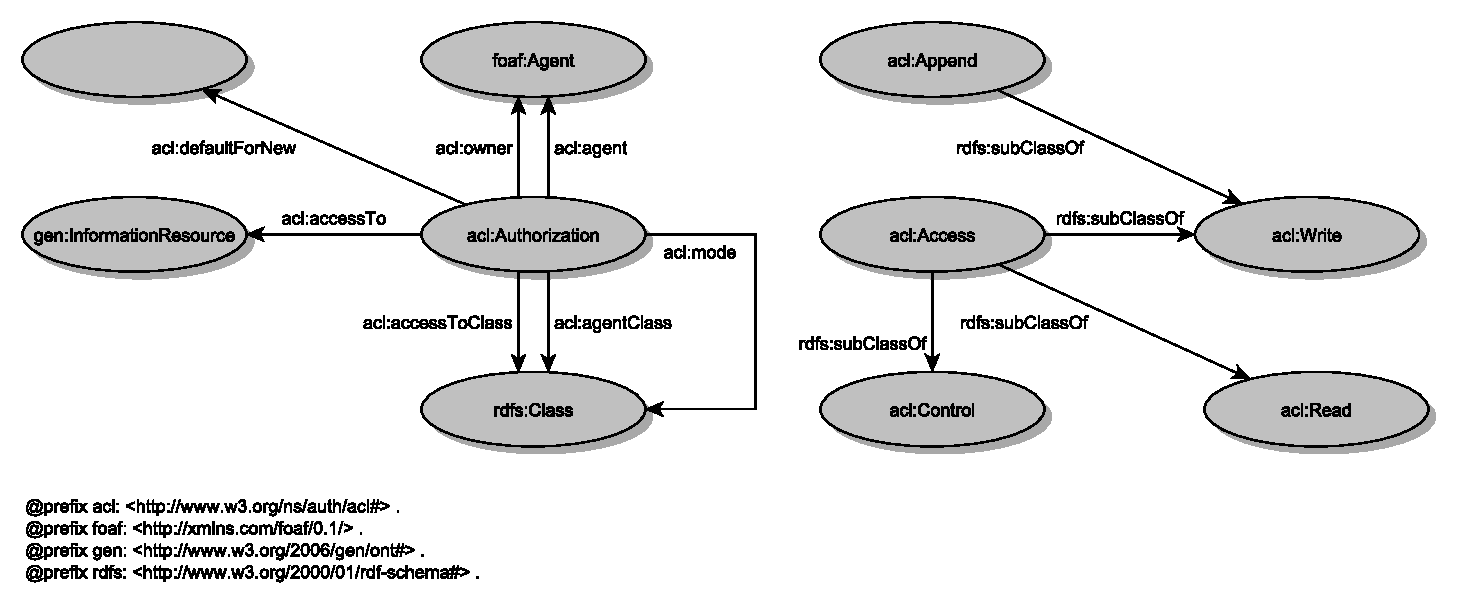
\includegraphics[
        width=\textwidth,
        keepaspectratio=true]
        {assets/images/w3c_web_acl}
    \caption{Basic Access Control Ontologie}
    \label{fig:w3c_web_acl}
\end{figure}

Zugriffsrechte für Ressourcen werden in dieser ACL mit der Klasse \texttt{acl:Access} modelliert. Von dieser Klasse werden einzelne Rechte wie \texttt{acl:Read} für das Lesen und \texttt{acl:Write} für das Schreiben abgeleitet. Nebenbei existieren noch die Ableitungen \texttt{acl:Control} für die Kontrolle über die ACL und \texttt{acl:Append} zum Anfügen von Daten an die Ressource. Die letzten beiden Rechte sind aber für SOCC unbedeutend.

Die Verbindung von einen Zugriffsrecht mit eine Ressource wird über die Klasse \texttt{acl:Authorization} erreicht. Der Besitzer dieser Autorisierung wird durch die Eigenschaft \texttt{alc:owner} festgelegt und gehört zur Klasse \texttt{foaf:Agent} beziehungsweise der davon abgeleiteten Klasse \texttt{foaf:Person}. Mittels der Eigenschaft \texttt{acl:agent} wird festgelegt für welche Person/Agenten diese Autorisierung gilt. Das selbe wird auch über die Eigenschaft \texttt{acl:agentClass} bestimmt, wobei hier eine abstrakte Klasse statt eine Instanz davon gemeint ist. Soll zum Beispiel der öffentlicher Zugriff für eine Ressource definiert werden, wird bei \texttt{acl:agentClass} die Klasse \texttt{foaf:Agent} eingesetzt (vgl. \cite[\enquote{Public Access}]{wiki:wacl}). Dies besagt, dass alle Agenten auf diese Ressource zugreifen können. Innerhalb von SOCC werden nur Ressourcen verarbeiten, die so öffentlich zugänglich gemacht wurden. Welches Recht für eine Ressource eingeräumt wird, kann über die Eigenschaft \texttt{acl:mode} festgelegt werden. SOCC testet aber nur ob das Recht \texttt{acl:Read} zum Lesen oder \texttt{acl:Write} zum Schreiben von Beiträgen eingeräumt wurde. Auf welche Ressource  sich letztendlich eine Autorisierung bezieht, wird über die Eigenschaft \texttt{acl:accessTo} geregelt. Die Angabe von \enquote{http://www.facebook.com} würde sich für SOCC zum Beispiel auf alle Beiträge des Besitzers auf Facebook beziehen, \enquote{https://canvas.instructure.com/courses/798152} dahingegen nur auf alle Beiträge innerhalb eines Canvas Kurses mit der ID \enquote{798152}. Für einen Zugriff auf alle Beiträge prüft SOCC, ob die Eigenschaft \texttt{acl:accessToClass} auf die Klasse \texttt{sioc:Post} verweist. So müsste nicht jede einzelne Webseite angegeben werden, wenn man ein generelles Zugriffsrecht auf seine Beiträge einräumen will.

Das Listing \ref{lst:acl_beispiel} zeigt ein Beispiel, wie eine Autorisierung mit der ACL in Turtle aussehen könnte. Der Besitzer dieser Autorisierung mit der URI \texttt{http:/example.org\#john} wird in Zeile 2 festgelegt. Er erlaubt damit SOCC einen öffentlichen (Zeile 3), lesenden (Zeile 4) Zugriff auf all seine geschrieben Beiträge (Zeile 5).

\begin{lstlisting}[
    caption={Basic Access Control Beispiel in Turtle }\label{lst:acl_beispiel},
    captionpos=t]
[] a acl:Authorization ;
    acl:owner <http:/example.org#john> ;
    acl:agentClass foaf:Agent ;
    acl:mode acl:Read ;
    acl:accessToClass sioc:Post .
\end{lstlisting}

% subsection autorisierung (end)

% section konfiguration (end)

\section{Design eines Connectors} % (fold)
\label{sec:design_eines_connectors}

\begin{wrapfigure}{r}{8cm}
    \centering
    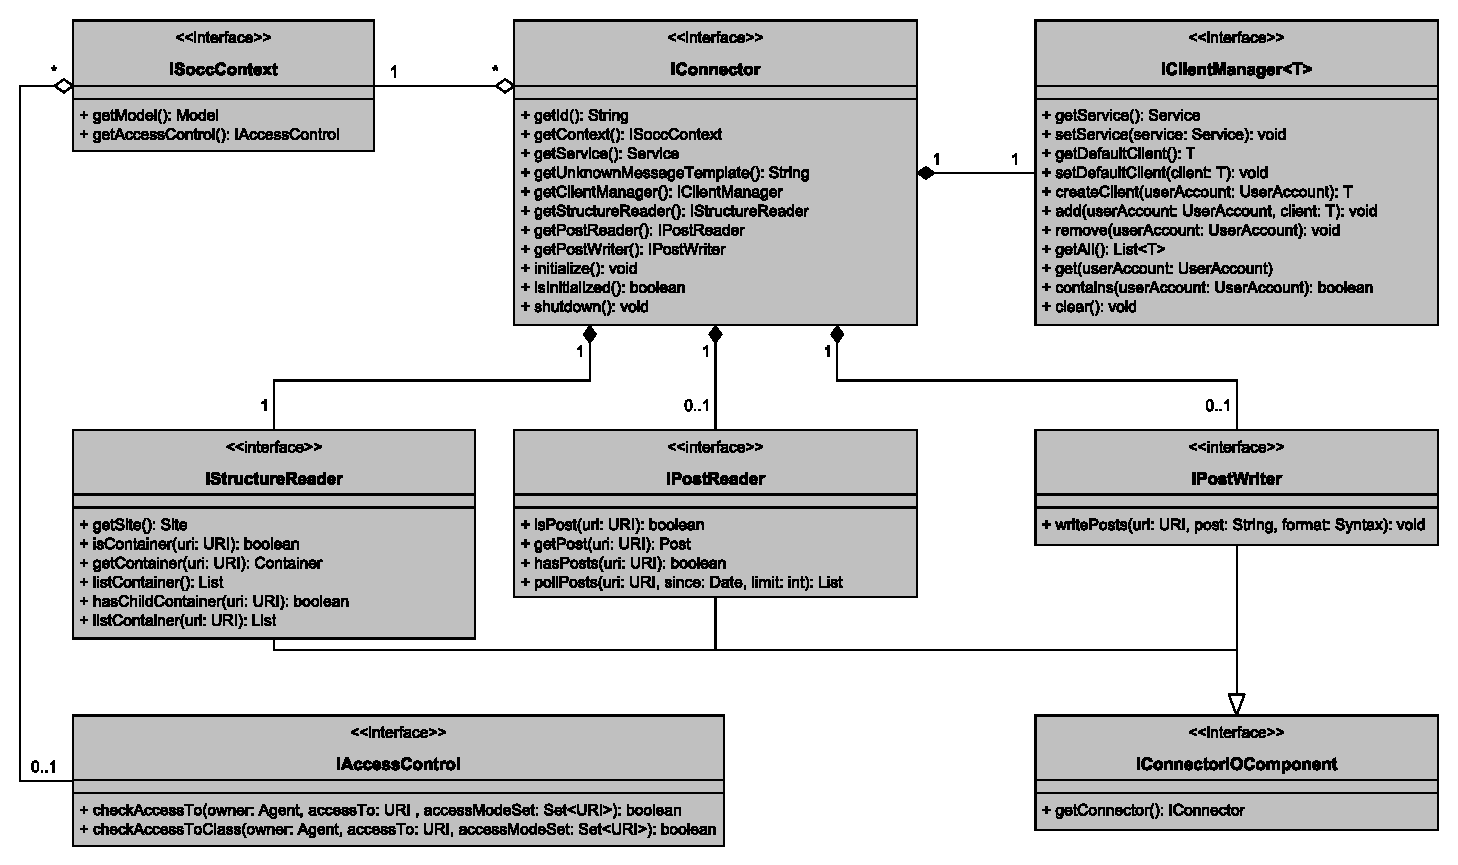
\includegraphics[
        width=8cm,
        keepaspectratio=true,
        clip=true,
        trim= 246 258 259 8]
    {assets/images/socc_uml_classdiagram}
    \caption{PostReader}
    \label{fig:uml_connector_interface}
\end{wrapfigure}

Die rechte Abbildung \ref{fig:uml_connector_interface} zeigt die Schnittstelle \texttt{IConnector} gegen die ein Connector implementiert werden muss. Sie bietet Zugriff auf die Eigenschaften die mit der Klasse \texttt{ccfg:ConnectorConfig} für die Konfiguration eines Connectors im Triplestore bereitgestellt werden. Diese Schnittstelle definiert Methodenüber welche die Komponenten zum Lesen der Seitenstruktur mit dem StructureReader sowie zum Lesen und Schreiben von Beiträgen mit PostReader und PostWriter zugänglich sind. Zuzüglich werden noch Methoden für den Zugriff auf Hilfskomponenten wie den \emph{SOCC Context}, \emph{AccessControl} und \emph{ClientManger} bereitgestellt. Das UML-Klassendiagramm in Abbildung \ref{fig:connector_uml_classdiagram} zeigt die Beziehung zwischen den Connector und den anderen Komponenten aus dem er besteht, welche in den folgenden Unterabschnitten noch weiter erklärt werden.

Für den Lebenszyklus eines Connectors sind noch die Methoden \texttt{initialize()} und \texttt{shutdown()} wichtig. Nach dem Erzeugen eines Connectors muss die Methode \texttt{initialize()} aufgerufen, um noch mögliche Vorarbeiten durchzuführen bevor der Connector genutzt werden kann. Ob ein Connector schon initialisiert wurde, kann mit der Methode \texttt{isInitialized()} überprüft werden. Bevor eine Connector gelöscht werden kann, sollte noch die Methode \texttt{shutdown()} aufgerufen werden. Sie dient dazu verwendete Ressourcen wieder freizugeben.

\begin{minipage}{\textwidth}
    \centering
    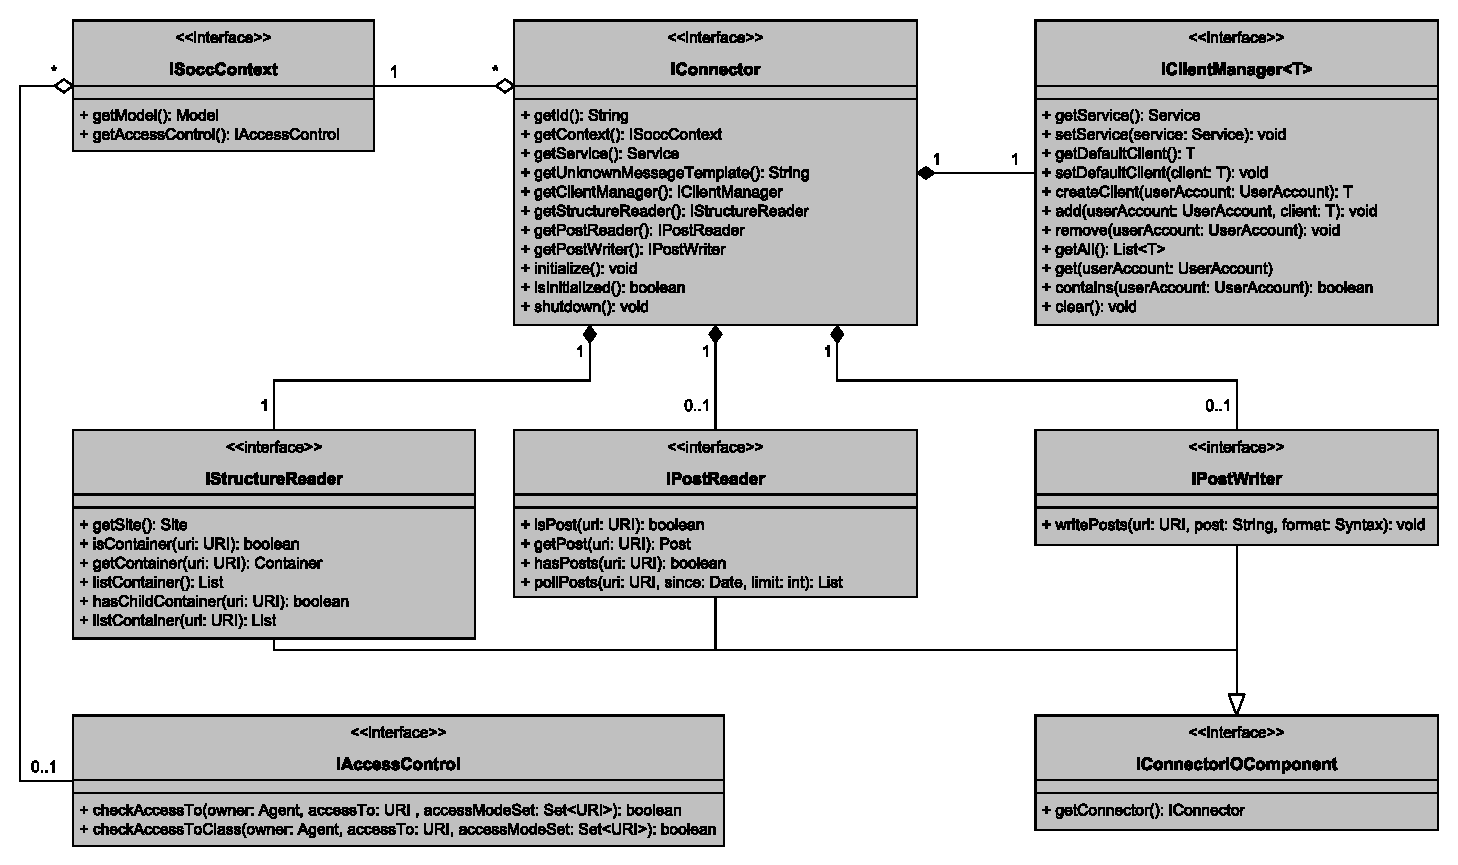
\includegraphics[
        scale=0.95,
        keepaspectratio=true,
        angle=90]
    {assets/images/socc_uml_classdiagram}
    \captionof{figure}{UML-Klassendiagramm eines Connectors}
    \label{fig:connector_uml_classdiagram}
\end{minipage}

% subsection design_eines_connectors (end)

\subsection{SOCC Context} % (fold)
\label{sub:socc_context}

\begin{wrapfigure}{r}{6cm}
    \centering
    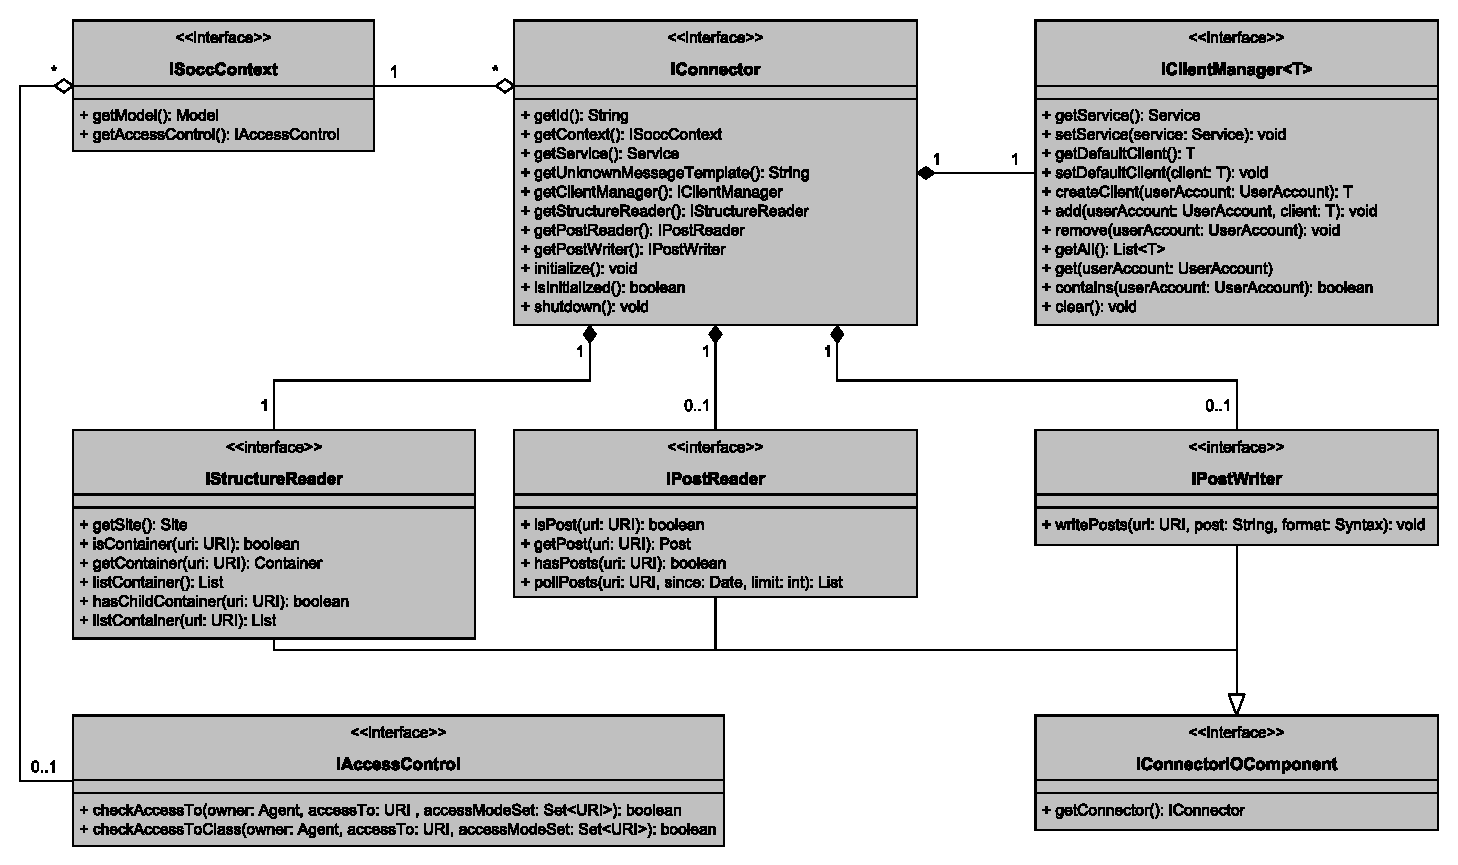
\includegraphics[
        width=6cm,
        keepaspectratio=true,
        clip=true,
        trim= 35 340 520 9]
    {assets/images/socc_uml_classdiagram}
    \caption{SOCC Context}
    \label{fig:uml_socc_context}
\end{wrapfigure}

Der SOCCContext eines Connectors, beschreibt die Umgebung die er zum Arbeiten braucht. Über ihn bekommt der Connector Zugriff auf den Triplestore, der durch die Klasse \texttt{Model} der RDF2Go Bibliothek abstrahiert wird (Siehe Abschnitt \ref{sec:verwendete_bibliotheken_und_programme}). In ihm befinden sich alle Daten die der Connector für seinen Betrieb benötigt und benutzt ihn gleichzeitig als Lagerplatz für Daten die während des Betriebs gespeichert werden müssen. Eine Referenz auf dieses Triplestore erhält der Connector über den Aufruf der Funktion \texttt{getModel()}. Durch die Methode \texttt{getAccessControl()} kann der Connector über die im folgenden Abschnitt beschriebene AccessControl-Schnittstelle auf die Information für die Autorisierung zugreifen. 

% subsubsection socc_context (end)

\subsection{AccessControl} % (fold)
\label{sub:accesscontrol}

\begin{wrapfigure}{r}{12cm}
    \centering
    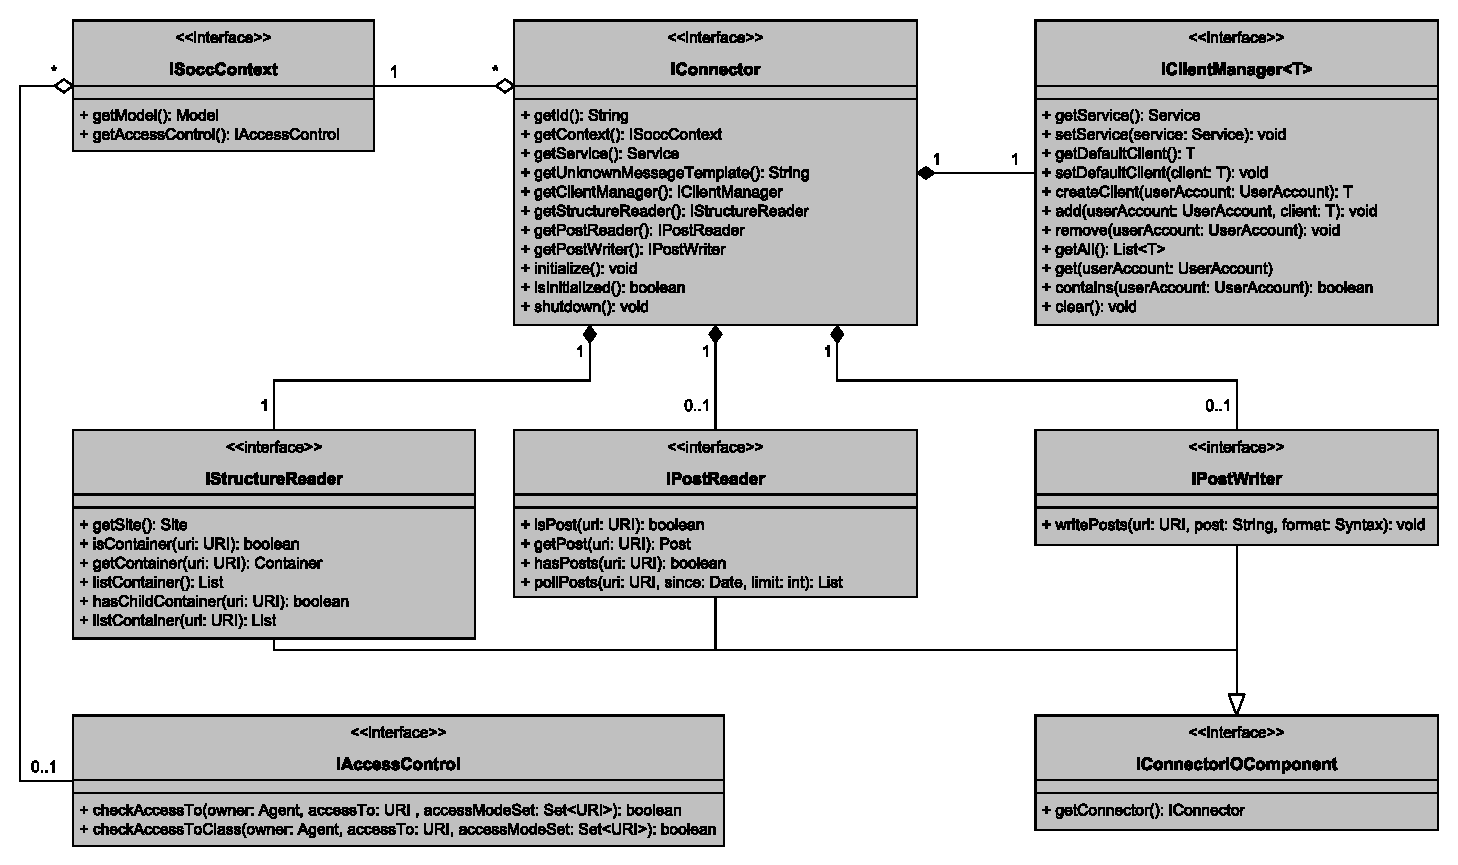
\includegraphics[
        width=12cm,
        keepaspectratio=true,
        clip=true,
        trim= 35 8 350 340]
    {assets/images/socc_uml_classdiagram}
    \caption{AccessControl}
    \label{fig:uml_accesscontrol}
\end{wrapfigure}

Die AccessControl-Schnittstelle ist sehr einfach gehalten und dient für den Zugriff auf die in Abschnitt \ref{sub:autorisierung} beschriebenen ACL-Information. Die Methode \texttt{checkAccessTo(\dots)} prüft, ob der Zugriff auf eine Ressource mit allen übergebenen Rechten erlaubt ist. Die andere Methode \texttt{checkAccessToClass} ist zur Überprüfung, ob die Rechte für den Zugriff auf eine komplette Klasse von Ressourcen vorhanden sind. 

% subsubsection accesscontrol (end)

\subsection{ClientManager} % (fold)
\label{sub:clientmanager}

\begin{wrapfigure}{r}{7cm}
    \centering
    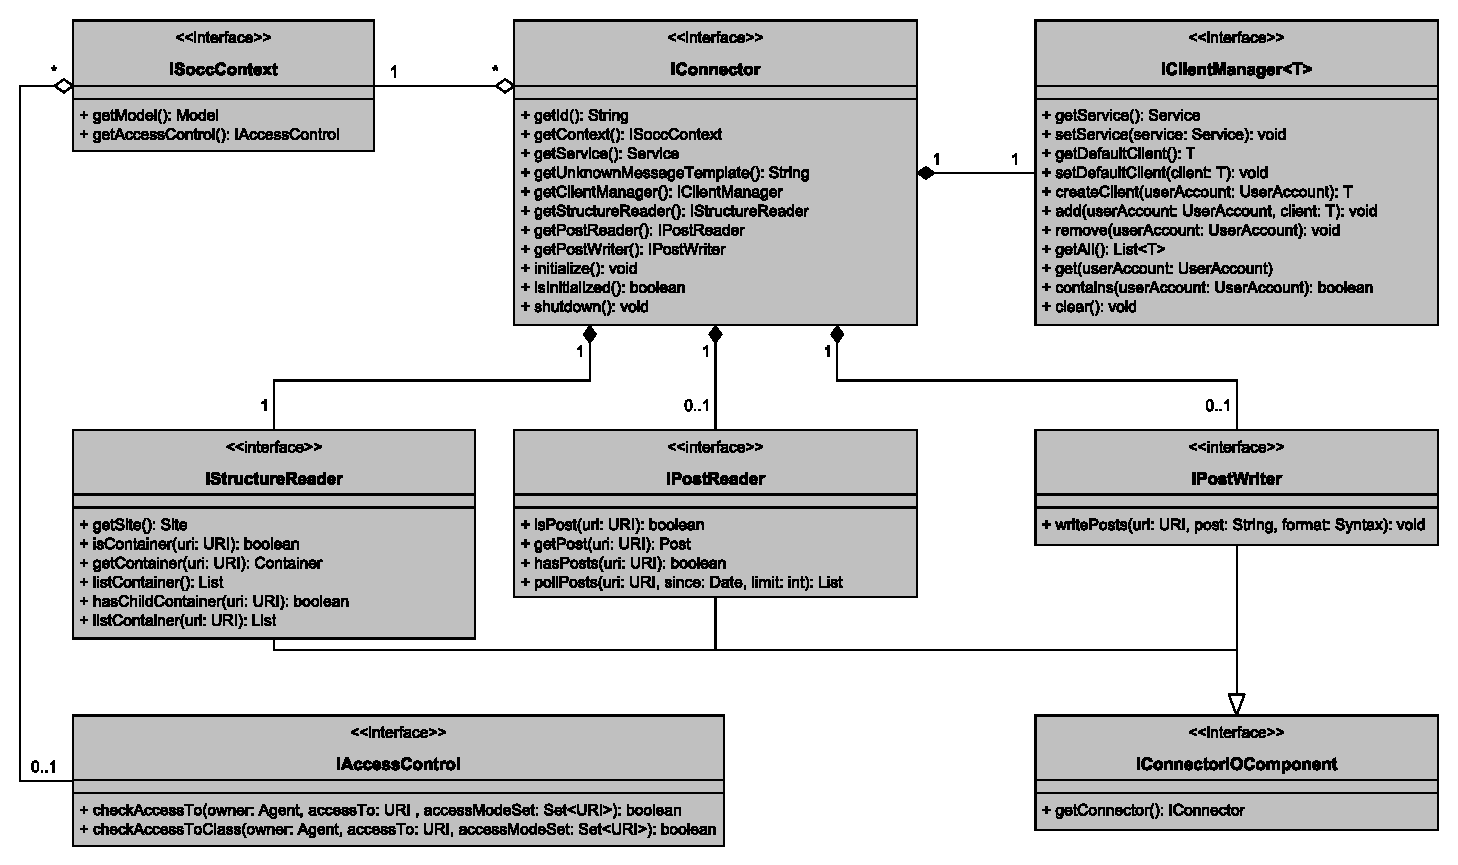
\includegraphics[
        width=7cm,
        keepaspectratio=true,
        clip=true,
        trim= 497 257 9 9]
    {assets/images/socc_uml_classdiagram}
    \caption{ClientManager}
    \label{fig:uml_clientmanager}
\end{wrapfigure}

Der Zugriff innerhalb des Programms auf eine API erfolgt in der Regel über einen Client. Dieser Client erlaubt es mit den Anmeldedaten für ein Benutzerkonto auf die Funktionen der API über verschiedene Methoden zu zugreifen. Da ein Client immer nur mit einem Benutzerkonto verknüpft ist und von diesen eine große Anzahl verwaltet werden müssen, enthält jeder Connector einen eigen ClientManager für diese Aufgaben. Für alle vom Benutzer unabhängigen Daten erhält der ClientManager ein wie Abschnitt \ref{sub:services} beschriebenes Objekt der Klasse Service das oftmals wichtige Daten wie ClientID und ClientSecret enthält. Das Erzeugen eines neuen Clients erfolgt dann durch den Aufruf der Methode \texttt{createClient(\dots)}. Als Parameter wird er ein Benutzerkonto (\texttt{sioc:UserAccount}) übergeben. Sind alle erforderlichen Authentifizierungsinformation aus Abschnitt \ref{sub:authentifizierung} vorhanden, wird ein neuer Client erstellt und zurück an den Aufrufer gegeben. Dieser Client wird aber dadurch nicht automatisch vom ClientManager verwaltet. Hierzu muss der im vorherigen Schritt erzeugte Client durch die Übergabe an \texttt{add(userAccount: UserAccount, client: T )} dauerhaft mit den angegeben Benutzerkonto verknüpft und intern gespeichert werden. In der aktuellen Implementierung ist es wichtig, dass die Eigenschaften \texttt{foaf:accountName} und \texttt{foaf:accountServiceHomepage} des \texttt{sioc:UserAccount}-Objekts gesetzt sind. Aus diesen wird ein eindeutiger Schlüssel generiert, der zur Zuordnung von Benutzerkonto und Client innerhalb des ClientManagers dient. Des weiteren stehen noch Methoden \texttt{remove(userAccount: UserAccount)} zum Entfernen, \texttt{get(userAccount: UserAccount)} zum Suchen von Clients sowie \texttt{contains(userAccount: UserAccount)} zum Testen, ob ein Client zu einem Benutzerkonto existiert zur Verfügung. Sollen zum Beispiel am Ende der Laufzeit des Programms alle erzeugten Clients auf einmal abgemeldet und gelöscht werden, kann dies über die Methode \texttt{clear()} erfolgen. Der ClientManager verwaltet ebenfalls den Client für den in Abschnitt \ref{sub:connector_config_ontologie} angesprochenen Defaultuser. Dieser \emph{Defaultclient} kann über die Methode  \texttt{setDefaultClient(client: T)} gesetzt und durch \texttt{getDefaultClient()} jederzeit wieder abgerufen werden. 

% subsubsection clientmanager (end)

\subsection{StructureReader} % (fold)
\label{sub:structurereader}

\begin{wrapfigure}[11]{r}{9cm}
    \centering
    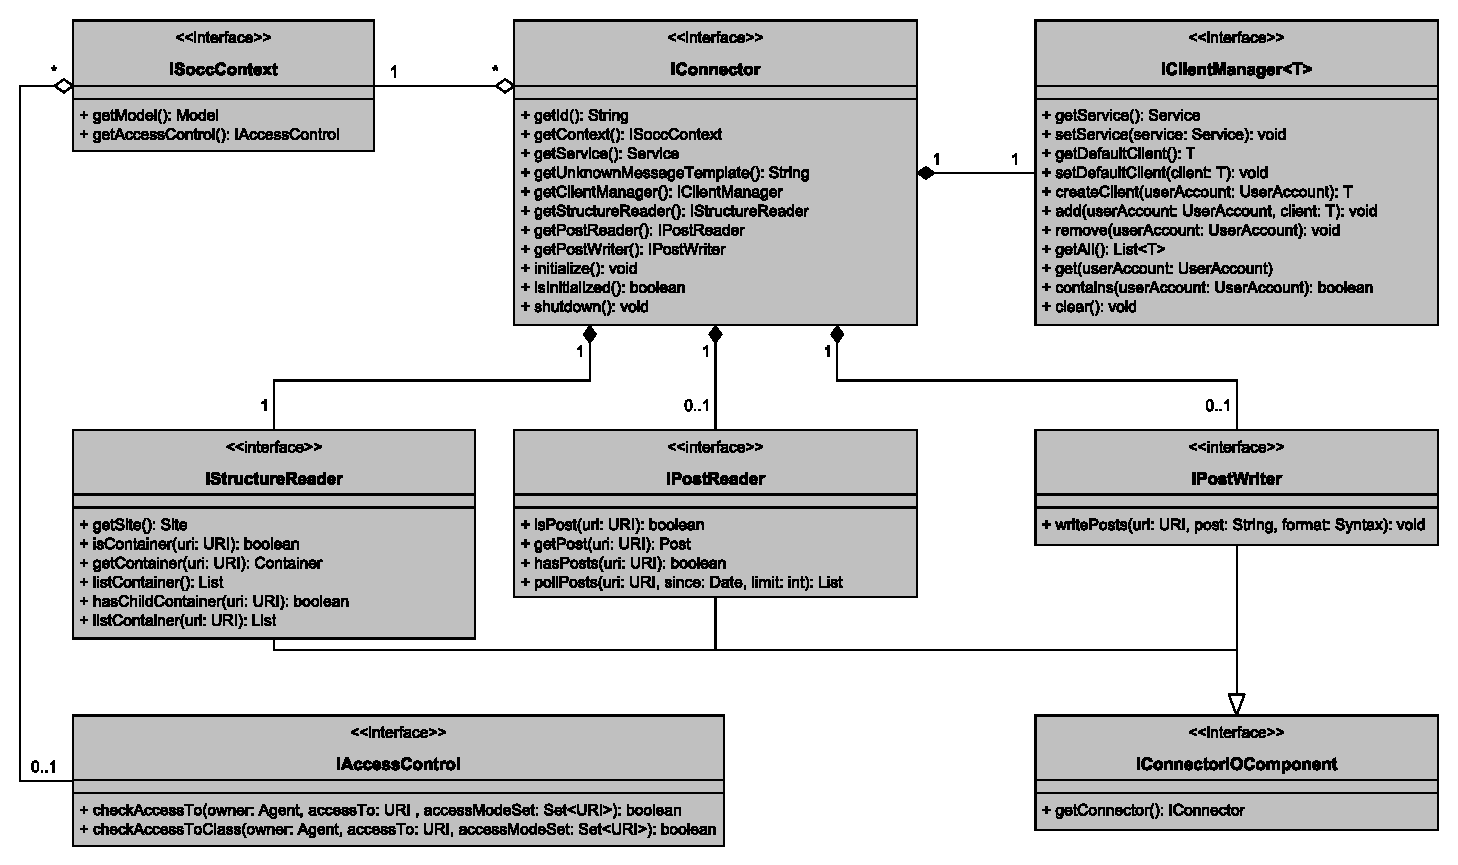
\includegraphics[
        width=9cm,
        keepaspectratio=true,
        clip=true,
        trim= 20 109 456 206]
    {assets/images/socc_uml_classdiagram}
    \caption{StructurReader}
    \label{fig:uml_structure_reader}
\end{wrapfigure}

Um auf Informationen über die Struktur von Foren, sozialen Online-Netzwerken und so weiter im SIOC-Format zugreifen zu können, implementiert jeder Connector dazu einen StructureReader. Die Struktur lässt sich, wie im Abschnitt \ref{ssub:semantically_interlinked_online_communities} vorgestellt, durch die SIOC Klassen \texttt{sioc:Site} und \texttt{sioc:Container} (sowie Unterklassen davon) beschreiben. Für den Zugriff auf diese Struktur, enthält der StructureReader mehrere Methoden die in der UML-Klasse rechts in Abbildung \ref{fig:uml_structure_reader}) zu sehen sind. \wrapfill

\begin{description}
    \item[\textbf{\texttt{getSite()}}] ist eine Methode, welche die Beschreibung einer Seite (Forum, Blog, soziales Online-Netzwerk) als Objekt der SIOC-Klasse \texttt{sioc:Site} zurücklieft. Dieses wird relativ häufig gebraucht, um die Zugehörigkeit anderer Objekte durch einen Verweis auf diese Seite zu verdeutlichen. Dies kann bei einigen APIs nützlich sein, da dort manchmal keine Information zum Ursprungsort eines Beitrags mitgeliefert werden, über den man sonst eine Beziehung zwischen Seite und Beitrag herstellen könnte.

    \item[\textbf{\texttt{isContainer(uri: URI)}}] wird zu Überprüfung verwendet, ob sich hinter einer URI ein potenzieller Container für Beiträge oder andere Container befindet. 

    \item[\textbf{\texttt{getContainer(URI)}}] liefert Informationen zu einen Container im SIOC-Format, der sich hinter der übergeben URI befindet.

    \item[\textbf{\texttt{hasChildContainer(uri: URI)}}] überprüft, ob der Container hinter der übergeben URI weitere Container als Kinder besitzt. Diese Methode wird dazu eingesetzt, um vorab zu testen, ob der Aufruf von \texttt{listContainer(URI)} das gewünschte Ergebnis liefert oder ein Fehler auftreten würde. 

    \item[\textbf{\texttt{listContainer(\dots)}}] sind Methoden, welche für den das Auflisten aller Container einer Seite (aus der Sicht des Defaultusers) zur Verfügung stehen. Die Methode ohne Parameter listet alle Container auf der ersten Ebene der Seitenstruktur auf . Dies könnten zum Beispiel alle Kurse innerhalb von Canvas oder alle beigetretenen Gruppen auf Facebook sein. Die zweite Methode mit einer URI als Parameter gibt eine Liste alle Container, welche den Container hinter der übergeben URI als Elternteil haben zurück. Dies könnten im Falle von Canvas alle Diskussionsthemen innerhalb eines Kurses sein.
\end{description}

% subsubsection structurereader (end)

\subsection{PostReader} % (fold)
\label{sub:postreader}

\begin{wrapfigure}{r}{9cm}
    \centering
    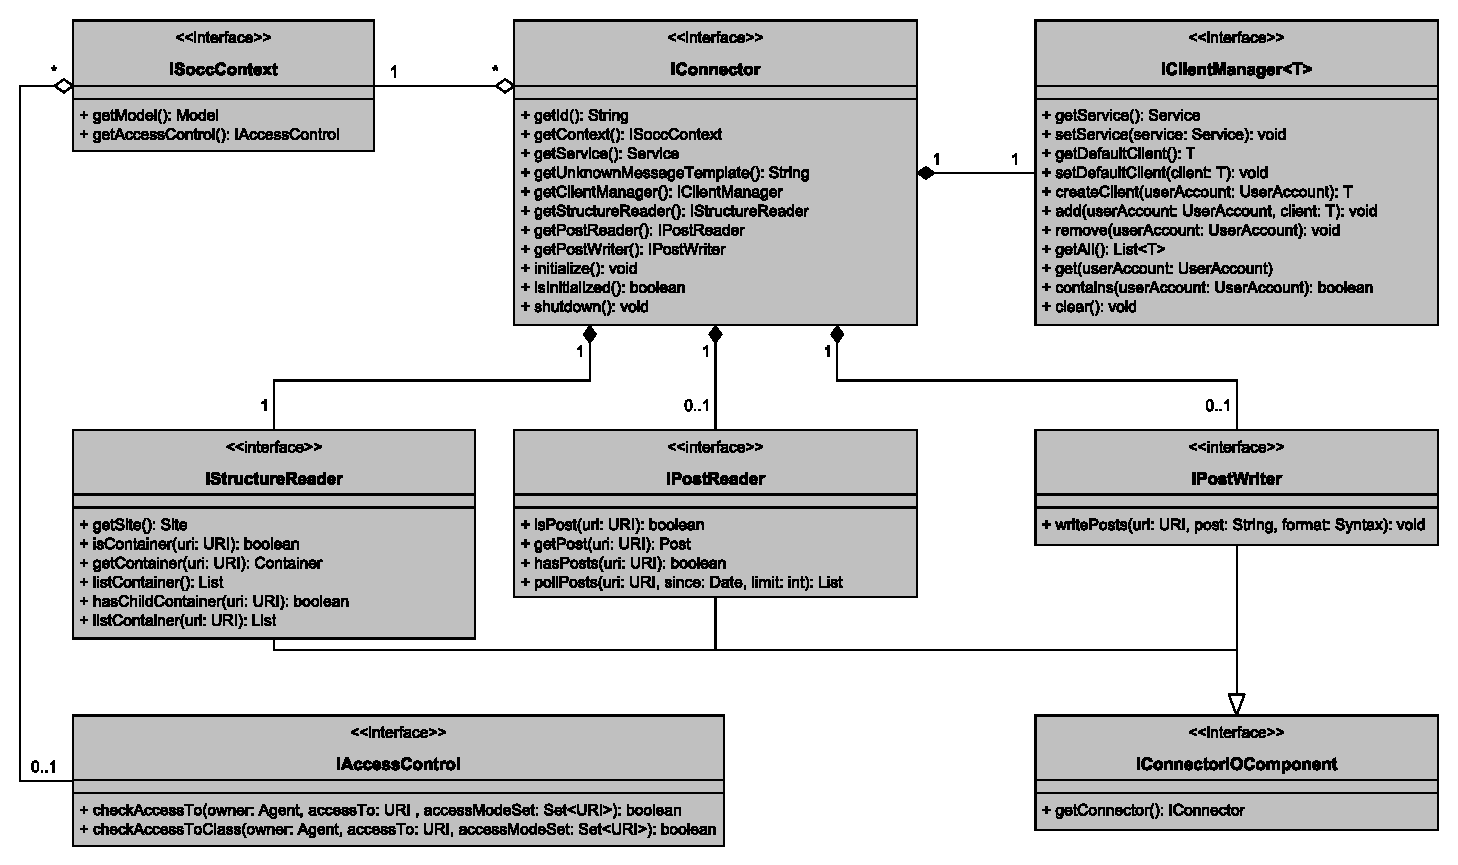
\includegraphics[
        width=9cm,
        keepaspectratio=true,
        clip=true,
        trim= 243 129 255 206]
    {assets/images/socc_uml_classdiagram}
    \caption{PostReader}
    \label{fig:uml_post_reader}
\end{wrapfigure}

Der \texttt{PostReader} dient als Schnittstelle für das Lesen geschriebener Beiträge innerhalb eines Containers oder der Kommentare auf einen anderen Beitrag. Er stellt nach außen hin Funktionen bereit mit denen entweder ein einzelner Beitrag oder alle Beiträge, die bestimmte Kriterien erfüllen, gelesen werden können. Bevor ein Beitrag zurück gegeben wird, müssen die Methoden prüfen, ob der Autor eines Beitrag das Lesen für diesen erlaubt hat. Falls nicht, wird der Beitrag aus der Ergebnisliste gelöscht. Die Funktionsweise der einzelnen Methoden ist wie folgt:

\begin{description}
    \item[\textbf{\texttt{isPost(uri: URI)}}] kann zur Überprüfung eingesetzt werden, ob sich hinter einer URI ein Beitrag befindet.

    \item[\textbf{\texttt{getPost(uri: URI)}}] ist dazu gedacht einen einzelnen Beitrag anhand seiner URI zu lesen. Sie liefert dann den Beitrag als Objekt der SIOC-Klasse \texttt{sioc:Post} zurück.

    \item[\textbf{\texttt{hasPost(uri: URI)}}] funktioniert ähnlich wie isPost, überprüft aber ob sich hinter der angegeben URI noch weitere Beiträge befinden können. 

    \item[\textbf{\texttt{pollPosts(uri: URI, since: Date, limit: int)}}] ist eine Methode die alle Beiträge hinter eine URI liest, welche die übergeben Kriterien erfüllen. Insgesamt erhält diese Methode drei Parameter. Der Erste ist eine URI die den Ort angibt, von der die Beiträge gelesen werden sollen. Mit dem zweiten Parameter kann ein Zeitpunkt angegeben werden, ab dem ein zu lesender Beitrag geschrieben sein muss. Zum Beispiel der Zeitpunkt als diese Methode das letzte mal aufgerufen wurde, um alle Beiträge die danach geschrieben wurden zu lesen. Der letzte Parameter gibt eine obere Schranke an, wie viele Beiträge maximal pro Aufruf dieser Methode gelesen werden dürfen. Ist dieses Limit erreicht, werden keine weiteren Beiträge in die Ergebnisliste aufgenommen.
\end{description}

% subsubsection postreader (end)

\subsection{PostWriter} % (fold)
\label{sub:postwriter}

In Abbildung \ref{fig:postwriter_sequenzdiagramm} ist ein UML-Sequenzdiagramm der PostWriter-Komponente zu sehen. Dort ist visualisiert, welche Schritte für das stellvertretende Schreiben von Beiträgen eines Benutzers unternommen werden müssen. Soll nun ein Beitrag in Plattform des Connectors geschrieben werden, wird die Methode \texttt{writePosts(URI, String, Syntax)} mit dem Zielort als URI, den Beiträgen als serialisierte RDF-Objekte und dem verwendeten Serialisierungsformat aufgerufen. Die folgenden Schritte werden dann für jeden \texttt{sioc:Post} in den serialisierten Daten durchgeführt:

Es beginnt damit, dass zuerst nach einem Benutzerkonto des Beitragautors für die Plattform des aktuellen Connectors gesucht wird. Dieser sollte im Idealfall im Triplestore des Connectors nach dem im Abschnitt \ref{sub:benutzerdaten} Schema vorliegen. Mit diesem Benutzerkonto, in Form der Klasse \texttt{sioc:UserAccount} aus SIOC, kann dann vom ClientManager ein Client für die verwendete API geholt werden. Sollte die Suche negativ verlaufen, steht noch der Defaultclient zur Verfügung. Bevor der Beitrag aber geschrieben werden kann, muss nachgeschaut werden, ob eine Erlaubnis für das Schreiben mit diesem Client vorliegt. Ist dies der Fall kann der Beitrag in das von der API verwendete Format konvertiert und an die richtige Stellen der Plattform geschrieben werden.

\begin{minipage}{\textwidth}
    \centering
    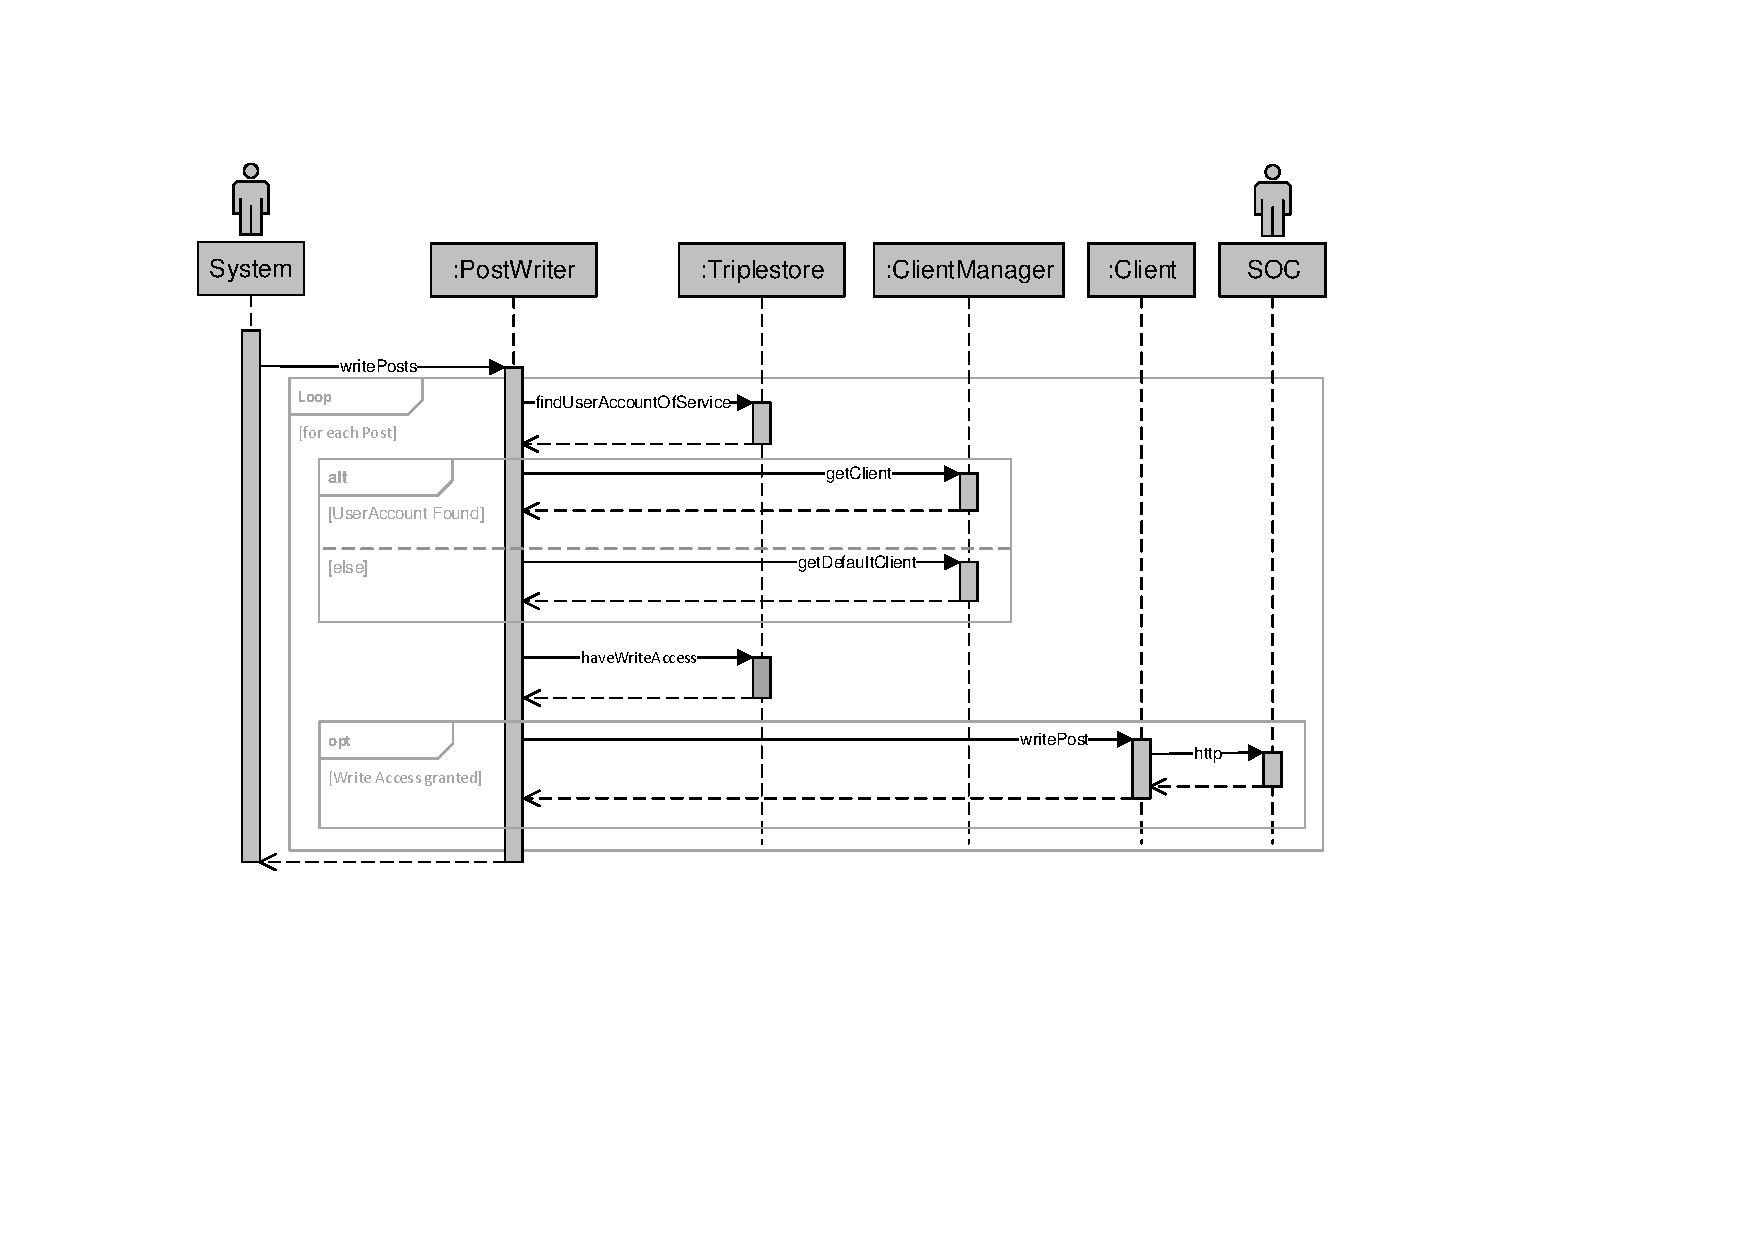
\includegraphics[
        width=\textwidth,
        keepaspectratio=true,
        clip=true,
        trim= 94 170 200 75]
    {assets/images/postwriter_sequencediagram}
    \captionof{figure}{UML-Sequenzdiagramm eines PostWriters}
    \label{fig:postwriter_sequenzdiagramm}
\end{minipage}

% subsubsection postwriter (end)

% subsection connector_aufbau (end)

% section social_online_community_connectors (end)

\section{SOCC-Camel} % (fold)
\label{sec:socc_camel}
%% korrigiert am 2013-09-26 22:04

\emph{SOCC-Camel} ist eine Modul von SOCC für die Integration von Connectoren in Camel. Durch dieses ist auf flexible Weise möglich die gelesenen Beiträge von einer Plattform über die Connectoren in eine andere zu schreiben. Die Abbildung \ref{fig:uebersicht_socc_camel} zeigt SOCC-Camel als EIP-Diagramm. 

\begin{minipage}{\textwidth}
    \centering
     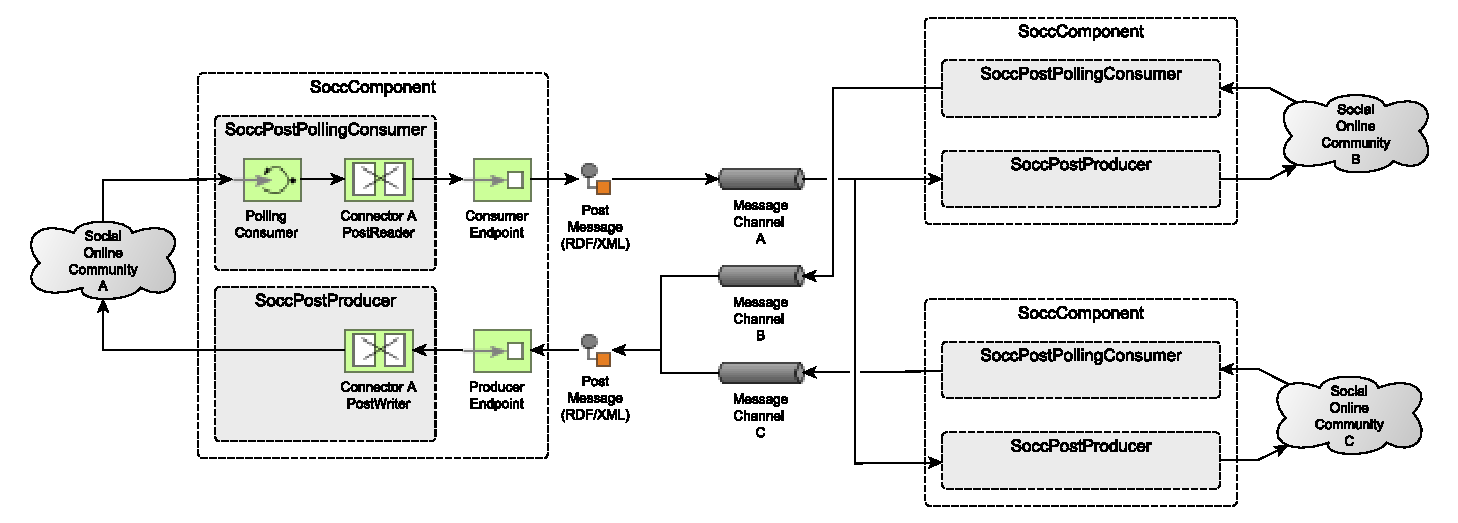
\includegraphics[
        width=\textwidth,
        keepaspectratio=true]
        {assets/images/socc_camel_overview}
    \captionof{figure}{Übersicht des SOCC-Camel Moduls als EIP-Diagramm.}
    \label{fig:uebersicht_socc_camel}
\end{minipage}

Hauptklasse dieses Moduls ist \texttt{SoccComponent}. Sie ist für die Verwaltung von Connectoren und Erstellen der Endpunkte für Camel zuständig. Von dieser Klasse muss zuerst ein Objekt erzeugt und ein SoccContext mit dem Tripelstore und alle Informationen für die Connectoren wie für deren Konfiguration, Benutzerkonten oder Servicebeschreibungen übergeben werden. Also alle Daten die in Anschnitt \ref{sec:konfiguration} beschrieben wurden. Das SoccComponent-Objekt wird dann unter einen frei wählbaren Namen in Camel registriert. Als Namen ist \enquote{socc} aber vorzuziehen.  Nun kann wie in Abschnitt \ref{ssub:apache_camel} mit dieser Komponente Routen zusammengesetzt werden.

Die URIs für die Konfiguration der Endpunkte mit SOCC-Camel habe dazu den folgenden Aufbau: \enquote{\texttt{socc://{connectorId}?uri={targetUri}[\&{parameter}...]}}. Der Anfang der URI mit \enquote{\texttt{socc://}} sagt Camel, dass es für diesen Endpunkt die Komponente benutzten soll, die vorher unter dem Namen \enquote{socc} registriert wurde - also SoccComponent. Für den Platzhalter \enquote{\{connectorId\}} muss eine gültige ID eines Connectors sein, dessen Konfigurationsdaten im TripleStore hinterlegt wurden. Über den Parameter \enquote{uri} wird dann die Quell- beziehungsweise Ziel-URI für den Connector angegeben, von der Beiträge gelesen beziehungsweise in die Beiträge geschrieben werden sollen. Je nach Endpunkt können dann noch weitere Parameter angegeben werden. Ein Endpunkt wird in SOCC-Camel durch die Klasse \texttt{SoccEndpoint} modelliert (nicht explizit in der Abbildung angegeben) und leitet sich von der Camel-Klasse \texttt{ScheduledPollEndpoint}, die das Verwenden der folgenden \texttt{SoccPostPollConsumer} Klasse vereinfacht.

\subsection{SoccPostPollConsumer} % (fold)
\label{sub:soccpostpollingconsumer}

Wird ein Endpunkt mit der Absicht zum Lesen von Beiträgen erstellt, erzeugt die Klasse SoccEndpoint ein Objekt der Klasse SoccPostPollConsumer und übergibt im die Parameter aus der Konfigurations-URI. Da SoccPostPollingConsumer sich von der Camel-Klasse \texttt{ScheduledPollConsumer} ableitet, ist es über den Parameter \texttt{delay} möglich in periodischen Abständen das Lesen von Beiträgen auszuführen. Die Angabe erfolgt dabei in Millisekunden. Der Parameter \texttt{limit} entspricht dabei den gleichnamigen Argument der Methode \texttt{pollPosts(\dots)} des PostReaders aus Abschnitt \ref{sub:postreader}. Das dort noch fehlende Argument \texttt{since}, für das Datum, ab wann ein Beitrag als neu gilt, wird mit dem Zeitpunkt belegt wann die Methode \texttt{pollPosts(\dots)} das letzte Mal aufgerufen wurde. Alle neuen, gelesenen Beiträge werden am Ende in das RDF/XML-Format serialisiert und als Nachricht an Camel übergeben. Damit andere Komponenten diese Nachricht wieder korrekt de-serialisieren können, muss der Nachricht noch ein Header mit dem Schlüssel \enquote{Content-Type} und dem MIME-Type\footnote{ Multipurpose Internet Mail Extension - Types: \url{http://tools.ietf.org/html/rfc2046}} vom RDF/XML \enquote{application/rdf+xml} als Wert mitgegeben werden.

% subsection soccpostpollconsumer (end)

\subsection{SoccPostProducer} % (fold)
\label{sub:soccpostproducer}

Der \texttt{SoccPostProducer} ist das Gegenstück zum SoccPostPollConsumer. Er ist der Endpunkt der zum Schreiben von Beiträgen in die Plattform des Connectors von der Klasse SoccEndpoint erzeugt wird. Intern verwendet er den PostWriter des betreffenden Connetors und leitet den Inhalt der Nachricht an diesen weiter. Außer der Angabe über die Ziel-URI erhält der SoccPostProducer keine weiteren Parameter über die Konfigurations-URI. Der SoccPostProducer überprüft auch ob ein gültiger MIME-Type angeben wurde. Akzeptiert wird auf jeden Fall \enquote{application/rdf+xml} für RDF/XML. Je nach verwendeten Adapter für RDF2Go können auch \enquote{"application/x-turtle"} für Turtle oder \enquote{application/rdf+json} für RDFJson\footnote{\url{https://dvcs.w3.org/hg/rdf/raw-file/default/rdf-json/index.html}} verwendet werden.

% subsection soccpostproducer (end)

% section socc_camel (end)

% chapter eigener_ansatz_social_online_community_connectors_socc_ (end)
		%!TEX root = ../thesis.tex

\chapter{Implementierung} % (fold)
\label{cha:implementierung}

\section{Verwendete Bibliotheken} % (fold)
\label{sec:verwendete_bibliotheken}

\subsection{RDF2Go} % (fold)
\label{sub:rdf2go}

% subsection rdf2go (end)



% section verwendete_bibliotheken (end)

\section{Implementierung der Connectoren} % (fold)
\label{sec:implementierung_der_connectoren}

Das muss rein:
\begin{itemize}
    \item Mapping nach SIOC
    \item Zugriff über die API
    \item Probleme bei der Implementierung
\end{itemize}

\subsection{Moodle} % (fold)
\label{sub:moodle_connector}

\begin{itemize}
    \item Eingebaute REST Schnittstelle, aber kein Lesen von Beiträgen
    \item WebService Plugin MoodleWS (REST oder SOAP)
    \begin{itemize}
        \item https://github.com/patrickpollet/moodlews
        \item ClientAPI existieren von selber Autor
        \item REST defekt, kein schreiben von Beiträgen möglich
        \item SOAP funktioniert mehr oder weniger
        \item Verschluckt Fehlermeldungen
        \item kein lesen einzelner Posts/Threads/Foren
        \item SOAP ClientAPI neu generieren, weil vorhandene nicht mit 2.4 funktioniert.
        \item Username/Password + Session Token/Id
        \item “Use an auto generated wsdl” -> No
        \item schreiben von neuen Beitrag direkt in thread nur als Antwort auf ersten Beitrag möglich
        \item Rückgabe aller Beiträge in einem Objekt
    \end{itemize}
\end{itemize}

\subsubsection{SIOC Mapping} % (fold)
\label{ssub:moodle_sioc_mapping}

\subsubsection{API} % (fold)
\label{ssub:moolde_api}

\subsubsection{Herausforderungen} % (fold)
\label{ssub:moodle_herausforderungen}

% subsubsection moodle_herausforderungen (end)

% subsubsection moodle_api (end)

% subsubsection moodle_sioc_mapping (end)

% subsection moodle_connector (end)

\subsection{Facebook} % (fold)
\label{sub:facebook_connector}

\begin{itemize}
    \item REST API + JSON
    \item keine offizielle Java API für Desktop -> Web + Mobile only
    \item GraphAPI, Facebook Query Language
    \item OAuth 2.x
    \begin{itemize}
        \item kein Refreshtoke
        \item Token Haltbarkeit 2h (2 Monate, wen extended)
        \item token nur über webbrowser
    \end{itemize}
    \item RestFB alternative Java API für die REST Schnittstelle der GraphAPI
    \item Typ der zurückgelieferten Daten nicht anhand der URI erkennbar, häufig erst durch Angabe von \emph{metadata=1}
    \item beim herunterladen einzelner Posts nicht immer erkennbar wo sie geschrieben wurden
\end{itemize}

\subsubsection{SIOC Mapping} % (fold)
\label{ssub:facebook_sioc_mapping}

\subsubsection{API} % (fold)
\label{ssub:facebook_api}

\subsubsection{Herausforderungen} % (fold)
\label{ssub:facebook_herausforderungen}

% subsubsection facebook_herausforderungen (end)

% subsubsection facebook_api (end)

% subsubsection facebook_sioc_mapping (end)

% subsection facebook_connector (end)

\subsection{Google+} % (fold)
\label{sub:google_plus_connector}

\begin{itemize}
    \item Einfach REST API + JSON
    \item OAuth
    \begin{itemize}
        \item Refreshtoken (token laufen quasi nie ab)
        \item holen von token ohne webbrowser möglich
    \end{itemize}
    \item Objekte aufgebaut aus Actor (wer machte was), Verb(wie machte er es), Object (wtas machte er) + Metadata
    \item verschieden Sprachen + Plattformen
    \item lesen nur von öffentlichen Beiträgen
    \item kein Schreiben von Beiträgen
\end{itemize}

\subsubsection{SIOC Mapping} % (fold)
\label{ssub:google_plus_sioc_mapping}

\subsubsection{API} % (fold)
\label{ssub:google_plus_api}

\subsubsection{Herausforderungen} % (fold)
\label{ssub:google_plus_herausforderungen}

% subsubsection google_plus_herausforderungen (end)

% subsubsection google_plus_api (end)

% subsubsection google_plus_sioc_mapping (end)

% subsection google_plus_connector (end)

\subsection{Youtube } % (fold)
\label{sub:youtube_connector}

\begin{itemize}
    \item Aktueller Umbau der API (ähnlich google+) v3
    \begin{itemize}
        \item keine lesen von kommentaren
        \item kein schreiben
    \end{itemize}
    \item alte GData Feed API v2 basiert auf RSS + Youtube Erweiterung
    \item Mapping teilweise durch basis auf RSS einfach, manchmal auch nicht
    \item Wichtigen Metadaten nur implizit vorhanden (comment id in uri aber nicht in datenformat)
\end{itemize}

\subsubsection{SIOC Mapping} % (fold)
\label{ssub:youtube_sioc_mapping}

\subsubsection{API} % (fold)
\label{ssub:youtube_api}

\subsubsection{Herausforderungen} % (fold)
\label{ssub:youtube_herausforderungen}

% subsubsection youtube_herausforderungen (end)

% subsubsection youtube_api (end)

% subsubsection youtube_sioc_mapping (end)

% subsection youtube_connector (end)

\subsection{Canvas} % (fold)
\label{sub:canvas_connector}

\begin{itemize}
    \item relativ neues LMS
    \item super Bedienung
    \item super REST API
    \item keine Java API
    \item rudimentäre Eigenentwicklung einer Java API, Funktionsweise ähnlich  G+
    \item viel API Funktionen wohl nicht extern nutzbar (UserProfil lesen, vll. Falsche Berechtigung -> test nötig)
\end{itemize}

\subsubsection{SIOC Mapping} % (fold)
\label{ssub:canvas_sioc_mapping}

\subsubsection{API} % (fold)
\label{ssub:canvas_api}

\subsubsection{Herausforderungen} % (fold)
\label{ssub:canvas_herausforderungen}

% subsubsection canvas_herausforderungen (end)

% subsubsection canvas_api (end)

% subsubsection canvas_sioc_mapping (end)

% subsection canvas_connector (end)

% section implementierung_einiger_connectoren (end)

% chapter implementierung (end)
		%!TEX root = ../thesis.tex

\chapter{Zusammenfassung und Ausblick} % (fold)
\label{cha:zusammenfassung_und_ausblick}

Im letzten Kapitel sollen noch einmal alle Ergebnisse diese Arbeit zusammengefasst und einen Ausblick auf weiterführende Themen gegeben werden. In der Einleitung wurde beschrieben, dass Diskussionen ein wichtiger Bestandteil des E-Learnings ist, aber diese oftmals auf verschiedene Plattformen verteilt stattfinden. Dadurch verpassen Personen, die nur auf einer dieser Plattformen präsent sind, vielleicht für sie wichtige Informationen auf einer anderen. Außerdem werden die selben Diskussionsthemen immer wieder an unterschiedlichen Orten an den unterschiedlichsten Orten doppelt und dreifach behandelt. Aus diesem Grund sollte ein System entwickelt werden das den Austausch von Diskussionen zwischen den unterschiedlichen Plattformen ermöglicht. 

In Kapitel \ref{cha:analyse} wurde analysiert, welche Schritte für eine solche Synchronisation nötig sind. Zuerst musste eine Zwischenformat gefunden werden in das die Daten der unterschiedlichen Plattformen konvertiert werden konnten, da dieser Weg effizienter ist, als die einzelnen Formate untereinander zu konvertieren. Also ein solches Zwischenformat bat sich die SIOC Ontologie in Verbindung mit FOAF wunderbar an. Ontologien bietet nicht nur einen guten Ansatz für die Integration von unterschiedlichen Datenformaten, mit RDF ist es sogar möglich dass Programme diese Daten verstehen und aus ihnen neues Wissen ableiten können. Um die Daten letztendlich in das Zwischenformat konvertieren und verarbeiten zu können, braucht es eine einheitliche Schnittstelle mit der dies umgesetzt werden kann. Zusätzlich wurde noch ein System gebraucht, dass die konvertierten Daten zwischen den Schnittstellen für die einzelnen Plattformen austauscht. Zu eignete sich der Austausch über Nachrichten am besten, da dadurch die einzelnen Schnittstellen zeitlich und räumlich entkoppelt werden konnten und nicht voneinander abhängig sind. Als Basis für dieses Nachrichtensystem wurde dann Apache Camel ausgewählt. Mit dieser Java-Bibliothek können die Routen, welche die Nachrichten nehmen, flexibel konfiguriert werden und sind so leicht erweiterbar. Privatsphäre spielt in der heutigen Zeit ebenfalls ein wichtige Rolle. Deswegen muss es Benutzern es ermöglicht werden das automatischen Lesen und/oder Schreiben für seine Beiträge zuzustimmen oder abzulehnen.

Das Kapitel \ref{cha:eigener_ansatz_social_online_community_connectors_socc_} widmet sich der Beschreibung des Systems, welches alle notwendigen Schritte und Anforderungen aus Kapiel \ref{cha:analyse} erfüllt. Dieses System, dass SOCC getauft wurde, besteht aus Connectoren die für das Lesen, Konvertieren und Schreiben für die Plattformen verantwortlich sind und einer Komponente die diese Connectoren in Apache Camel integriert. 


\section{Ausblick} % (fold)
\label{sec:ausblick}

% section ausblick (end)

% chapter abschlussbetrachtung (end)
		\cleardoublepage

	\appendix
	    %!TEX root = ../thesis.tex

\chapter{Anhang} % (fold)
\label{cha:anhang}

\section{SOCC Connector Config Ontologie} % (fold)
\label{sec:anhang_socc_connector_config_ontologie}

\lstinputlisting[language=XML]{assets/listings/socc-config.owl}

% section socc_connector_config_ontologie (end)

\section{SIOC Services Authentication Module} % (fold)
\label{sec:anhang_sioc_services_authentication_module}

\lstinputlisting[language=XML]{assets/listings/sioc-service-auth.owl}

% section sioc_services_authentication_module (end)

\section{Proof of Concept: Konfigurationsdaten} % (fold)
\label{sec:anhang_proof_of_concept_konfigurationsdaten}

\lstinputlisting[language={}]{assets/listings/poc_config_model.ttl}

% section proof_of_concept_konfigurationsdaten (end)

% chapter anhang (end)
		%!TEX root = ../thesis.tex

%\addcontentsline{toc}{chapter}{Literaturverzeichnis}
\bibliographystyle{plain}
\bibliography{bibliography/bibliography}

\end{document}

% Einleitung
%     (Motivation)
%     (Anforderungen)
%     (Kapitelübersicht)

% Grundlagen und verwandte Arbeiten
%     Datenintegration 
%         (Zusammenführen von Daten aus verschiedenen Quellen)
%         RDF
%         SIOC
%     Verwandte Arbeiten/Projekte
%         Reclaim
%         Glue!-PS

% Analyse
%     (Was fehlt bei verwandten Arbeiten)
%     Einheitliche Schnittstelle
%     MessagePassing
%         JMS vs Apache Camel  vs JMS + Apache Camel

% Eigener Ansatz
%     Verwendung von SIOC (RDF2Go...)
%     Connectoren Konzept
%         Moodle
%         Canvas LMS
%         Facebook
%         Youtube
%         Google+

% Evaluation
%     Auswertung was alles erreicht wurde

% Fazit und Ausblick